\documentclass[twoside]{book}

% Packages required by doxygen
\usepackage{fixltx2e}
\usepackage{calc}
\usepackage{doxygen}
\usepackage[export]{adjustbox} % also loads graphicx
\usepackage{graphicx}
\usepackage[utf8]{inputenc}
\usepackage{makeidx}
\usepackage{multicol}
\usepackage{multirow}
\PassOptionsToPackage{warn}{textcomp}
\usepackage{textcomp}
\usepackage[nointegrals]{wasysym}
\usepackage[table]{xcolor}

% Font selection
\usepackage[T1]{fontenc}
\usepackage[scaled=.90]{helvet}
\usepackage{courier}
\usepackage{amssymb}
\usepackage{sectsty}
\renewcommand{\familydefault}{\sfdefault}
\allsectionsfont{%
  \fontseries{bc}\selectfont%
  \color{darkgray}%
}
\renewcommand{\DoxyLabelFont}{%
  \fontseries{bc}\selectfont%
  \color{darkgray}%
}
\newcommand{\+}{\discretionary{\mbox{\scriptsize$\hookleftarrow$}}{}{}}

% Page & text layout
\usepackage{geometry}
\geometry{%
  a4paper,%
  top=2.5cm,%
  bottom=2.5cm,%
  left=2.5cm,%
  right=2.5cm%
}
\tolerance=750
\hfuzz=15pt
\hbadness=750
\setlength{\emergencystretch}{15pt}
\setlength{\parindent}{0cm}
\setlength{\parskip}{3ex plus 2ex minus 2ex}
\makeatletter
\renewcommand{\paragraph}{%
  \@startsection{paragraph}{4}{0ex}{-1.0ex}{1.0ex}{%
    \normalfont\normalsize\bfseries\SS@parafont%
  }%
}
\renewcommand{\subparagraph}{%
  \@startsection{subparagraph}{5}{0ex}{-1.0ex}{1.0ex}{%
    \normalfont\normalsize\bfseries\SS@subparafont%
  }%
}
\makeatother

% Headers & footers
\usepackage{fancyhdr}
\pagestyle{fancyplain}
\fancyhead[LE]{\fancyplain{}{\bfseries\thepage}}
\fancyhead[CE]{\fancyplain{}{}}
\fancyhead[RE]{\fancyplain{}{\bfseries\leftmark}}
\fancyhead[LO]{\fancyplain{}{\bfseries\rightmark}}
\fancyhead[CO]{\fancyplain{}{}}
\fancyhead[RO]{\fancyplain{}{\bfseries\thepage}}
\fancyfoot[LE]{\fancyplain{}{}}
\fancyfoot[CE]{\fancyplain{}{}}
\fancyfoot[RE]{\fancyplain{}{\bfseries\scriptsize Generated by Doxygen }}
\fancyfoot[LO]{\fancyplain{}{\bfseries\scriptsize Generated by Doxygen }}
\fancyfoot[CO]{\fancyplain{}{}}
\fancyfoot[RO]{\fancyplain{}{}}
\renewcommand{\footrulewidth}{0.4pt}
\renewcommand{\chaptermark}[1]{%
  \markboth{#1}{}%
}
\renewcommand{\sectionmark}[1]{%
  \markright{\thesection\ #1}%
}

% Indices & bibliography
\usepackage{natbib}
\usepackage[titles]{tocloft}
\setcounter{tocdepth}{3}
\setcounter{secnumdepth}{5}
\makeindex

% Hyperlinks (required, but should be loaded last)
\usepackage{ifpdf}
\ifpdf
  \usepackage[pdftex,pagebackref=true]{hyperref}
\else
  \usepackage[ps2pdf,pagebackref=true]{hyperref}
\fi
\hypersetup{%
  colorlinks=true,%
  linkcolor=blue,%
  citecolor=blue,%
  unicode%
}

% Custom commands
\newcommand{\clearemptydoublepage}{%
  \newpage{\pagestyle{empty}\cleardoublepage}%
}

\usepackage{caption}
\captionsetup{labelsep=space,justification=centering,font={bf},singlelinecheck=off,skip=4pt,position=top}

%===== C O N T E N T S =====

\begin{document}

% Titlepage & ToC
\hypersetup{pageanchor=false,
             bookmarksnumbered=true,
             pdfencoding=unicode
            }
\pagenumbering{alph}
\begin{titlepage}
\vspace*{7cm}
\begin{center}%
{\Large Coinche.\+N\+ET \\[1ex]\large 1.\+0 }\\
\vspace*{1cm}
{\large Generated by Doxygen 1.8.13}\\
\end{center}
\end{titlepage}
\clearemptydoublepage
\pagenumbering{roman}
\tableofcontents
\clearemptydoublepage
\pagenumbering{arabic}
\hypersetup{pageanchor=true}

%--- Begin generated contents ---
\chapter{Namespace Index}
\section{Namespace List}
Here is a list of all documented namespaces with brief descriptions\+:\begin{DoxyCompactList}
\item\contentsline{section}{\hyperlink{namespace_coinche}{Coinche} }{\pageref{namespace_coinche}}{}
\item\contentsline{section}{\hyperlink{namespace_coinche_1_1_client}{Coinche.\+Client} }{\pageref{namespace_coinche_1_1_client}}{}
\item\contentsline{section}{\hyperlink{namespace_coinche_1_1_google}{Coinche.\+Google} }{\pageref{namespace_coinche_1_1_google}}{}
\item\contentsline{section}{\hyperlink{namespace_coinche_1_1_google_1_1_protobuf}{Coinche.\+Google.\+Protobuf} }{\pageref{namespace_coinche_1_1_google_1_1_protobuf}}{}
\item\contentsline{section}{\hyperlink{namespace_coinche_1_1_server}{Coinche.\+Server} }{\pageref{namespace_coinche_1_1_server}}{}
\item\contentsline{section}{\hyperlink{namespace_coinche_1_1_tools}{Coinche.\+Tools} }{\pageref{namespace_coinche_1_1_tools}}{}
\item\contentsline{section}{\hyperlink{namespace_server}{Server} }{\pageref{namespace_server}}{}
\item\contentsline{section}{\hyperlink{namespace_server_1_1_game_rules}{Server.\+Game\+Rules} }{\pageref{namespace_server_1_1_game_rules}}{}
\item\contentsline{section}{\hyperlink{namespace_server_1_1_game_rules_1_1_steps}{Server.\+Game\+Rules.\+Steps} }{\pageref{namespace_server_1_1_game_rules_1_1_steps}}{}
\item\contentsline{section}{\hyperlink{namespace_server_1_1_game_rules_1_1_steps_1_1_counter}{Server.\+Game\+Rules.\+Steps.\+Counter} }{\pageref{namespace_server_1_1_game_rules_1_1_steps_1_1_counter}}{}
\end{DoxyCompactList}

\chapter{Hierarchical Index}
\section{Class Hierarchy}
This inheritance list is sorted roughly, but not completely, alphabetically\+:\begin{DoxyCompactList}
\item \contentsline{section}{Coinche.\+Board}{\pageref{class_coinche_1_1_board}}{}
\item \contentsline{section}{Coinche.\+Card}{\pageref{class_coinche_1_1_card}}{}
\item \contentsline{section}{Coinche.\+Google.\+Protobuf.\+Coinche\+Protocol\+Reflection}{\pageref{class_coinche_1_1_google_1_1_protobuf_1_1_coinche_protocol_reflection}}{}
\item \contentsline{section}{Coinche.\+Deck}{\pageref{class_coinche_1_1_deck}}{}
\item \contentsline{section}{Coinche.\+Tools.\+Game\+Info}{\pageref{class_coinche_1_1_tools_1_1_game_info}}{}
\item \contentsline{section}{Coinche.\+Server.\+Game\+Room}{\pageref{class_coinche_1_1_server_1_1_game_room}}{}
\item \contentsline{section}{Coinche.\+Game\+Rules}{\pageref{class_coinche_1_1_game_rules}}{}
\item I\+Message\begin{DoxyCompactList}
\item \contentsline{section}{Coinche.\+Google.\+Protobuf.\+Game\+Request}{\pageref{class_coinche_1_1_google_1_1_protobuf_1_1_game_request}}{}
\item \contentsline{section}{Coinche.\+Google.\+Protobuf.\+Game\+Request}{\pageref{class_coinche_1_1_google_1_1_protobuf_1_1_game_request}}{}
\item \contentsline{section}{Coinche.\+Google.\+Protobuf.\+Game\+Response}{\pageref{class_coinche_1_1_google_1_1_protobuf_1_1_game_response}}{}
\item \contentsline{section}{Coinche.\+Google.\+Protobuf.\+Game\+Response}{\pageref{class_coinche_1_1_google_1_1_protobuf_1_1_game_response}}{}
\end{DoxyCompactList}
\item \contentsline{section}{Coinche.\+I\+Step}{\pageref{interface_coinche_1_1_i_step}}{}
\begin{DoxyCompactList}
\item \contentsline{section}{Coinche.\+Announce}{\pageref{class_coinche_1_1_announce}}{}
\item \contentsline{section}{Coinche.\+Auction}{\pageref{class_coinche_1_1_auction}}{}
\item \contentsline{section}{Coinche.\+Tricks}{\pageref{class_coinche_1_1_tricks}}{}
\item \contentsline{section}{Server.\+Game\+Rules.\+Steps.\+Counter.\+Counter}{\pageref{class_server_1_1_game_rules_1_1_steps_1_1_counter_1_1_counter}}{}
\end{DoxyCompactList}
\item \contentsline{section}{Coinche.\+Tools.\+Logger}{\pageref{class_coinche_1_1_tools_1_1_logger}}{}
\item \contentsline{section}{Coinche.\+Player}{\pageref{class_coinche_1_1_player}}{}
\item \contentsline{section}{Coinche.\+Server.\+Program}{\pageref{class_coinche_1_1_server_1_1_program}}{}
\item \contentsline{section}{Coinche.\+Client.\+Program}{\pageref{class_coinche_1_1_client_1_1_program}}{}
\item Simple\+Channel\+Inbound\+Handler\begin{DoxyCompactList}
\item \contentsline{section}{Coinche.\+Client.\+Game\+Client}{\pageref{class_coinche_1_1_client_1_1_game_client}}{}
\item \contentsline{section}{Coinche.\+Server.\+Game\+Manager}{\pageref{class_coinche_1_1_server_1_1_game_manager}}{}
\end{DoxyCompactList}
\item \contentsline{section}{Coinche.\+Steps}{\pageref{class_coinche_1_1_steps}}{}
\end{DoxyCompactList}

\chapter{Class Index}
\section{Class List}
Here are the classes, structs, unions and interfaces with brief descriptions\+:\begin{DoxyCompactList}
\item\contentsline{section}{\hyperlink{class_coinche_1_1_announce}{Coinche.\+Announce} }{\pageref{class_coinche_1_1_announce}}{}
\item\contentsline{section}{\hyperlink{class_coinche_1_1_auction}{Coinche.\+Auction} }{\pageref{class_coinche_1_1_auction}}{}
\item\contentsline{section}{\hyperlink{class_coinche_1_1_board}{Coinche.\+Board} \\*class representing the board }{\pageref{class_coinche_1_1_board}}{}
\item\contentsline{section}{\hyperlink{class_coinche_1_1_card}{Coinche.\+Card} \\*class defining a card }{\pageref{class_coinche_1_1_card}}{}
\item\contentsline{section}{\hyperlink{class_coinche_1_1_google_1_1_protobuf_1_1_coinche_protocol_reflection}{Coinche.\+Google.\+Protobuf.\+Coinche\+Protocol\+Reflection} \\*Holder for reflection information generated from Coinche\+Protocol.\+proto}{\pageref{class_coinche_1_1_google_1_1_protobuf_1_1_coinche_protocol_reflection}}{}
\item\contentsline{section}{\hyperlink{class_server_1_1_game_rules_1_1_steps_1_1_counter_1_1_counter}{Server.\+Game\+Rules.\+Steps.\+Counter.\+Counter} \\*class representing the tricks step }{\pageref{class_server_1_1_game_rules_1_1_steps_1_1_counter_1_1_counter}}{}
\item\contentsline{section}{\hyperlink{class_coinche_1_1_deck}{Coinche.\+Deck} \\*class defining the deck }{\pageref{class_coinche_1_1_deck}}{}
\item\contentsline{section}{\hyperlink{class_coinche_1_1_client_1_1_game_client}{Coinche.\+Client.\+Game\+Client} \\*Game client. }{\pageref{class_coinche_1_1_client_1_1_game_client}}{}
\item\contentsline{section}{\hyperlink{class_coinche_1_1_tools_1_1_game_info}{Coinche.\+Tools.\+Game\+Info} \\*Tes messages to send to the players and the infos to update the game }{\pageref{class_coinche_1_1_tools_1_1_game_info}}{}
\item\contentsline{section}{\hyperlink{class_coinche_1_1_server_1_1_game_manager}{Coinche.\+Server.\+Game\+Manager} \\*Class to handle new connections comming from different clients }{\pageref{class_coinche_1_1_server_1_1_game_manager}}{}
\item\contentsline{section}{\hyperlink{class_coinche_1_1_google_1_1_protobuf_1_1_game_request}{Coinche.\+Google.\+Protobuf.\+Game\+Request} }{\pageref{class_coinche_1_1_google_1_1_protobuf_1_1_game_request}}{}
\item\contentsline{section}{\hyperlink{class_coinche_1_1_google_1_1_protobuf_1_1_game_response}{Coinche.\+Google.\+Protobuf.\+Game\+Response} }{\pageref{class_coinche_1_1_google_1_1_protobuf_1_1_game_response}}{}
\item\contentsline{section}{\hyperlink{class_coinche_1_1_server_1_1_game_room}{Coinche.\+Server.\+Game\+Room} \\*This class represents a \hyperlink{class_coinche_1_1_server_1_1_game_room}{Game\+Room} which role is to let 4 players play together. This let us abstract all the administration part of people joining and leaving a game. Once 4 players are connected to the same \hyperlink{class_coinche_1_1_server_1_1_game_room}{Game\+Room}, {\bfseries a game starts} If{\bfseries any player} leaves during the game, the session is restarted for everyone in the room. }{\pageref{class_coinche_1_1_server_1_1_game_room}}{}
\item\contentsline{section}{\hyperlink{class_coinche_1_1_game_rules}{Coinche.\+Game\+Rules} \\*class representing the game rules }{\pageref{class_coinche_1_1_game_rules}}{}
\item\contentsline{section}{\hyperlink{interface_coinche_1_1_i_step}{Coinche.\+I\+Step} \\*interface of each step }{\pageref{interface_coinche_1_1_i_step}}{}
\item\contentsline{section}{\hyperlink{class_coinche_1_1_tools_1_1_logger}{Coinche.\+Tools.\+Logger} \\*A simple \hyperlink{class_coinche_1_1_tools_1_1_logger}{Logger}. }{\pageref{class_coinche_1_1_tools_1_1_logger}}{}
\item\contentsline{section}{\hyperlink{class_coinche_1_1_player}{Coinche.\+Player} \\*class defining a player }{\pageref{class_coinche_1_1_player}}{}
\item\contentsline{section}{\hyperlink{class_coinche_1_1_server_1_1_program}{Coinche.\+Server.\+Program} \\*J\+Coinche \hyperlink{namespace_coinche_1_1_server}{Server} main class }{\pageref{class_coinche_1_1_server_1_1_program}}{}
\item\contentsline{section}{\hyperlink{class_coinche_1_1_client_1_1_program}{Coinche.\+Client.\+Program} \\*Jcoinche \hyperlink{namespace_coinche_1_1_client}{Client} Main \hyperlink{class_coinche_1_1_client_1_1_program}{Program} }{\pageref{class_coinche_1_1_client_1_1_program}}{}
\item\contentsline{section}{\hyperlink{class_coinche_1_1_steps}{Coinche.\+Steps} \\*class in which there is all the steps of the game }{\pageref{class_coinche_1_1_steps}}{}
\item\contentsline{section}{\hyperlink{class_coinche_1_1_tricks}{Coinche.\+Tricks} \\*class representing the tricks step }{\pageref{class_coinche_1_1_tricks}}{}
\end{DoxyCompactList}

\chapter{Namespace Documentation}
\hypertarget{namespace_coinche}{}\section{Coinche Namespace Reference}
\label{namespace_coinche}\index{Coinche@{Coinche}}
\subsection*{Namespaces}
\begin{DoxyCompactItemize}
\end{DoxyCompactItemize}
\subsection*{Classes}
\begin{DoxyCompactItemize}
\item 
class \hyperlink{class_coinche_1_1_announce}{Announce}
\item 
class \hyperlink{class_coinche_1_1_auction}{Auction}
\item 
class \hyperlink{class_coinche_1_1_board}{Board}
\begin{DoxyCompactList}\small\item\em class representing the board \end{DoxyCompactList}\item 
class \hyperlink{class_coinche_1_1_card}{Card}
\begin{DoxyCompactList}\small\item\em class defining a card \end{DoxyCompactList}\item 
class \hyperlink{class_coinche_1_1_deck}{Deck}
\begin{DoxyCompactList}\small\item\em class defining the deck \end{DoxyCompactList}\item 
class \hyperlink{class_coinche_1_1_game_rules}{Game\+Rules}
\begin{DoxyCompactList}\small\item\em class representing the game rules \end{DoxyCompactList}\item 
interface \hyperlink{interface_coinche_1_1_i_step}{I\+Step}
\begin{DoxyCompactList}\small\item\em interface of each step \end{DoxyCompactList}\item 
class \hyperlink{class_coinche_1_1_player}{Player}
\begin{DoxyCompactList}\small\item\em class defining a player \end{DoxyCompactList}\item 
class \hyperlink{class_coinche_1_1_steps}{Steps}
\begin{DoxyCompactList}\small\item\em class in which there is all the steps of the game \end{DoxyCompactList}\item 
class \hyperlink{class_coinche_1_1_tricks}{Tricks}
\begin{DoxyCompactList}\small\item\em class representing the tricks step \end{DoxyCompactList}\end{DoxyCompactItemize}
\subsection*{Enumerations}
\begin{DoxyCompactItemize}
\item 
\mbox{\Hypertarget{namespace_coinche_a74688723547f1c0e41be07e2db50ff84}\label{namespace_coinche_a74688723547f1c0e41be07e2db50ff84}} 
enum {\bfseries Card\+Color} \{ {\bfseries Heart}, 
{\bfseries Spade}, 
{\bfseries Diamond}, 
{\bfseries Club}
 \}
\item 
\mbox{\Hypertarget{namespace_coinche_a518a3d6f6210ba36deb1e7fc33a589eb}\label{namespace_coinche_a518a3d6f6210ba36deb1e7fc33a589eb}} 
enum {\bfseries Card\+Value} \{ \newline
{\bfseries Seven} = 0, 
{\bfseries Eight} = 1, 
{\bfseries Nine} = 2, 
{\bfseries Ten} = 3, 
\newline
{\bfseries Jack} = 4, 
{\bfseries Queen} = 5, 
{\bfseries King} = 6, 
{\bfseries Ace} = 7
 \}
\item 
\mbox{\Hypertarget{namespace_coinche_a08dfdc6c41e627cdae450a8dba7ff85e}\label{namespace_coinche_a08dfdc6c41e627cdae450a8dba7ff85e}} 
enum {\bfseries Step} \{ {\bfseries Auction} = 0, 
{\bfseries Counter} = 1, 
{\bfseries Announce} = 2, 
{\bfseries Tricks} = 3
 \}
\end{DoxyCompactItemize}

\hypertarget{namespace_coinche_1_1_client}{}\section{Coinche.\+Client Namespace Reference}
\label{namespace_coinche_1_1_client}\index{Coinche.\+Client@{Coinche.\+Client}}
\subsection*{Classes}
\begin{DoxyCompactItemize}
\item 
class \hyperlink{class_coinche_1_1_client_1_1_game_client}{Game\+Client}
\begin{DoxyCompactList}\small\item\em Game client. \end{DoxyCompactList}\item 
class \hyperlink{class_coinche_1_1_client_1_1_program}{Program}
\begin{DoxyCompactList}\small\item\em Jcoinche \hyperlink{namespace_coinche_1_1_client}{Client} Main \hyperlink{class_coinche_1_1_client_1_1_program}{Program} \end{DoxyCompactList}\end{DoxyCompactItemize}

\hypertarget{namespace_coinche_1_1_google}{}\section{Coinche.\+Google Namespace Reference}
\label{namespace_coinche_1_1_google}\index{Coinche.\+Google@{Coinche.\+Google}}
\subsection*{Namespaces}
\begin{DoxyCompactItemize}
\end{DoxyCompactItemize}

\hypertarget{namespace_coinche_1_1_google_1_1_protobuf}{}\section{Coinche.\+Google.\+Protobuf Namespace Reference}
\label{namespace_coinche_1_1_google_1_1_protobuf}\index{Coinche.\+Google.\+Protobuf@{Coinche.\+Google.\+Protobuf}}
\subsection*{Classes}
\begin{DoxyCompactItemize}
\item 
class \hyperlink{class_coinche_1_1_google_1_1_protobuf_1_1_coinche_protocol_reflection}{Coinche\+Protocol\+Reflection}
\begin{DoxyCompactList}\small\item\em Holder for reflection information generated from Coinche\+Protocol.\+proto\end{DoxyCompactList}\item 
class \hyperlink{class_coinche_1_1_google_1_1_protobuf_1_1_game_request}{Game\+Request}
\item 
class \hyperlink{class_coinche_1_1_google_1_1_protobuf_1_1_game_response}{Game\+Response}
\end{DoxyCompactItemize}

\hypertarget{namespace_coinche_1_1_server}{}\section{Coinche.\+Server Namespace Reference}
\label{namespace_coinche_1_1_server}\index{Coinche.\+Server@{Coinche.\+Server}}
\subsection*{Classes}
\begin{DoxyCompactItemize}
\item 
class \hyperlink{class_coinche_1_1_server_1_1_game_manager}{Game\+Manager}
\begin{DoxyCompactList}\small\item\em Class to handle new connections comming from different clients \end{DoxyCompactList}\item 
class \hyperlink{class_coinche_1_1_server_1_1_game_room}{Game\+Room}
\begin{DoxyCompactList}\small\item\em This class represents a \hyperlink{class_coinche_1_1_server_1_1_game_room}{Game\+Room} which role is to let 4 players play together. This let us abstract all the administration part of people joining and leaving a game. Once 4 players are connected to the same \hyperlink{class_coinche_1_1_server_1_1_game_room}{Game\+Room}, {\bfseries a game starts} If{\bfseries any player} leaves during the game, the session is restarted for everyone in the room. \end{DoxyCompactList}\item 
class \hyperlink{class_coinche_1_1_server_1_1_program}{Program}
\begin{DoxyCompactList}\small\item\em J\+Coinche \hyperlink{namespace_coinche_1_1_server}{Server} main class \end{DoxyCompactList}\end{DoxyCompactItemize}

\hypertarget{namespace_coinche_1_1_tools}{}\section{Coinche.\+Tools Namespace Reference}
\label{namespace_coinche_1_1_tools}\index{Coinche.\+Tools@{Coinche.\+Tools}}
\subsection*{Classes}
\begin{DoxyCompactItemize}
\item 
class \hyperlink{class_coinche_1_1_tools_1_1_game_info}{Game\+Info}
\begin{DoxyCompactList}\small\item\em Tes messages to send to the players and the infos to update the game \end{DoxyCompactList}\item 
class \hyperlink{class_coinche_1_1_tools_1_1_logger}{Logger}
\begin{DoxyCompactList}\small\item\em A simple \hyperlink{class_coinche_1_1_tools_1_1_logger}{Logger}. \end{DoxyCompactList}\end{DoxyCompactItemize}

\hypertarget{namespace_server}{}\section{Server Namespace Reference}
\label{namespace_server}\index{Server@{Server}}
\subsection*{Namespaces}
\begin{DoxyCompactItemize}
\end{DoxyCompactItemize}

\hypertarget{namespace_server_1_1_game_rules}{}\section{Server.\+Game\+Rules Namespace Reference}
\label{namespace_server_1_1_game_rules}\index{Server.\+Game\+Rules@{Server.\+Game\+Rules}}
\subsection*{Namespaces}
\begin{DoxyCompactItemize}
\end{DoxyCompactItemize}

\hypertarget{namespace_server_1_1_game_rules_1_1_steps}{}\section{Server.\+Game\+Rules.\+Steps Namespace Reference}
\label{namespace_server_1_1_game_rules_1_1_steps}\index{Server.\+Game\+Rules.\+Steps@{Server.\+Game\+Rules.\+Steps}}
\subsection*{Namespaces}
\begin{DoxyCompactItemize}
\end{DoxyCompactItemize}

\hypertarget{namespace_server_1_1_game_rules_1_1_steps_1_1_counter}{}\section{Server.\+Game\+Rules.\+Steps.\+Counter Namespace Reference}
\label{namespace_server_1_1_game_rules_1_1_steps_1_1_counter}\index{Server.\+Game\+Rules.\+Steps.\+Counter@{Server.\+Game\+Rules.\+Steps.\+Counter}}
\subsection*{Classes}
\begin{DoxyCompactItemize}
\item 
class \hyperlink{class_server_1_1_game_rules_1_1_steps_1_1_counter_1_1_counter}{Counter}
\begin{DoxyCompactList}\small\item\em class representing the tricks step \end{DoxyCompactList}\end{DoxyCompactItemize}

\chapter{Class Documentation}
\hypertarget{class_coinche_1_1_announce}{}\section{Coinche.\+Announce Class Reference}
\label{class_coinche_1_1_announce}\index{Coinche.\+Announce@{Coinche.\+Announce}}
Inheritance diagram for Coinche.\+Announce\+:\begin{figure}[H]
\begin{center}
\leavevmode
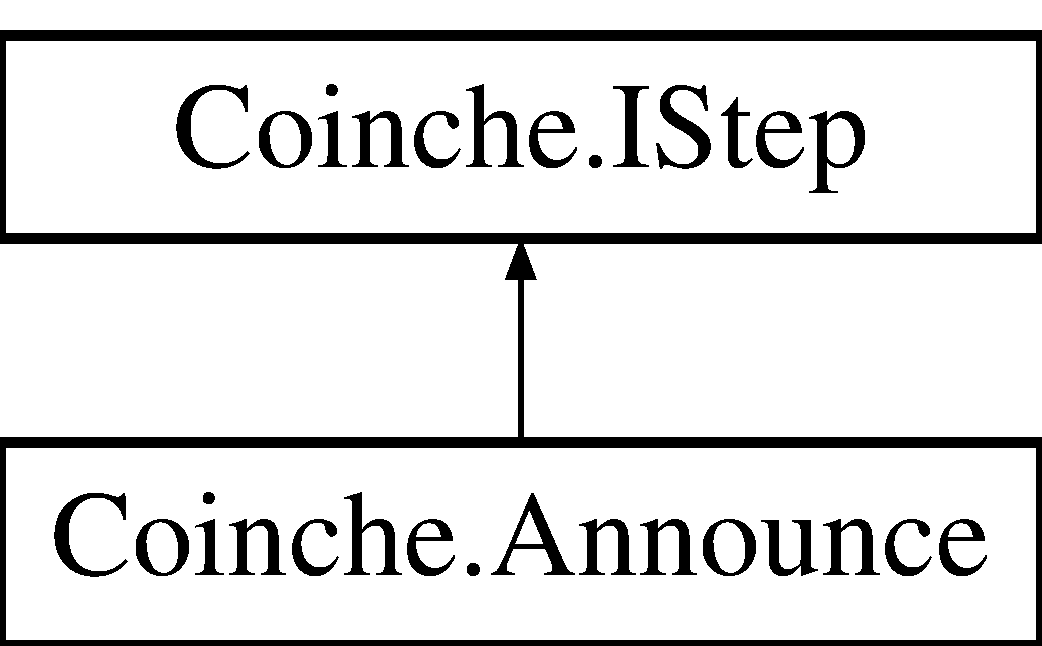
\includegraphics[height=2.000000cm]{class_coinche_1_1_announce}
\end{center}
\end{figure}
\subsection*{Private Member Functions}
\begin{DoxyCompactItemize}
\item 
void I\+Step. \hyperlink{class_coinche_1_1_announce_a0fddda733e5f081be1091b2c67279982}{Reset} ()
\begin{DoxyCompactList}\small\item\em reset the step \end{DoxyCompactList}\item 
\hyperlink{class_coinche_1_1_tools_1_1_game_info}{Game\+Info} I\+Step. \hyperlink{class_coinche_1_1_announce_a24398cfbd8280465732c360858e72e13}{Prepare\+Step} (\hyperlink{class_coinche_1_1_player}{Player} player, int team\+Contract)
\begin{DoxyCompactList}\small\item\em prepare the players for the next step \end{DoxyCompactList}\item 
\hyperlink{class_coinche_1_1_tools_1_1_game_info}{Game\+Info} I\+Step. \hyperlink{class_coinche_1_1_announce_acf172bfff869b6e3f63ac4a18de63a55}{Do\+Step} (\hyperlink{class_coinche_1_1_player}{Player} player, string msg, Boolean all\+Assets, Boolean none\+Assets, Card\+Color color\+Bet, int first\+Player)
\begin{DoxyCompactList}\small\item\em rules of the current step applied with the players messages \end{DoxyCompactList}\item 
\hyperlink{class_coinche_1_1_tools_1_1_game_info}{Game\+Info} I\+Step. \hyperlink{class_coinche_1_1_announce_a778b04cb7ff3405d1a182e445a7c8f4c}{Invalid\+Turn} (\hyperlink{class_coinche_1_1_player}{Player} player)
\begin{DoxyCompactList}\small\item\em function called if it wasn\textquotesingle{}t the right turn to play \end{DoxyCompactList}\item 
string I\+Step. \hyperlink{class_coinche_1_1_announce_a3337d94429e31a70eb66ee0be3714e86}{Step\+Over} ()
\begin{DoxyCompactList}\small\item\em function called when the step is over \end{DoxyCompactList}\end{DoxyCompactItemize}
\subsection*{Additional Inherited Members}


\subsection{Member Function Documentation}
\mbox{\Hypertarget{class_coinche_1_1_announce_acf172bfff869b6e3f63ac4a18de63a55}\label{class_coinche_1_1_announce_acf172bfff869b6e3f63ac4a18de63a55}} 
\index{Coinche\+::\+Announce@{Coinche\+::\+Announce}!Do\+Step@{Do\+Step}}
\index{Do\+Step@{Do\+Step}!Coinche\+::\+Announce@{Coinche\+::\+Announce}}
\subsubsection{\texorpdfstring{Do\+Step()}{DoStep()}}
{\footnotesize\ttfamily \hyperlink{class_coinche_1_1_tools_1_1_game_info}{Game\+Info} I\+Step. Coinche.\+Announce.\+Do\+Step (\begin{DoxyParamCaption}\item[{\hyperlink{class_coinche_1_1_player}{Player}}]{player,  }\item[{string}]{msg,  }\item[{Boolean}]{all\+Assets,  }\item[{Boolean}]{none\+Assets,  }\item[{Card\+Color}]{color\+Bet,  }\item[{int}]{first\+Player }\end{DoxyParamCaption})\hspace{0.3cm}{\ttfamily [inline]}, {\ttfamily [private]}}



rules of the current step applied with the players messages 


\begin{DoxyParams}{Parameters}
{\em player} & \\
\hline
{\em msg} & \\
\hline
{\em all\+Assets} & \\
\hline
{\em none\+Assets} & \\
\hline
{\em color\+Bet} & \\
\hline
{\em first\+Player} & \\
\hline
\end{DoxyParams}
\begin{DoxyReturn}{Returns}
a Game\+Info instance to tell players what happened
\end{DoxyReturn}


Implements \hyperlink{interface_coinche_1_1_i_step_a1b410159a7988ae4e75154539715e7ba}{Coinche.\+I\+Step}.

\mbox{\Hypertarget{class_coinche_1_1_announce_a778b04cb7ff3405d1a182e445a7c8f4c}\label{class_coinche_1_1_announce_a778b04cb7ff3405d1a182e445a7c8f4c}} 
\index{Coinche\+::\+Announce@{Coinche\+::\+Announce}!Invalid\+Turn@{Invalid\+Turn}}
\index{Invalid\+Turn@{Invalid\+Turn}!Coinche\+::\+Announce@{Coinche\+::\+Announce}}
\subsubsection{\texorpdfstring{Invalid\+Turn()}{InvalidTurn()}}
{\footnotesize\ttfamily \hyperlink{class_coinche_1_1_tools_1_1_game_info}{Game\+Info} I\+Step. Coinche.\+Announce.\+Invalid\+Turn (\begin{DoxyParamCaption}\item[{\hyperlink{class_coinche_1_1_player}{Player}}]{player }\end{DoxyParamCaption})\hspace{0.3cm}{\ttfamily [inline]}, {\ttfamily [private]}}



function called if it wasn\textquotesingle{}t the right turn to play 


\begin{DoxyParams}{Parameters}
{\em player} & \\
\hline
\end{DoxyParams}
\begin{DoxyReturn}{Returns}
a Game\+Info instance to inform the player it wasn\textquotesingle{}t his turn to play
\end{DoxyReturn}


Implements \hyperlink{interface_coinche_1_1_i_step_afc64813670860f5ee0829264751abc0a}{Coinche.\+I\+Step}.

\mbox{\Hypertarget{class_coinche_1_1_announce_a24398cfbd8280465732c360858e72e13}\label{class_coinche_1_1_announce_a24398cfbd8280465732c360858e72e13}} 
\index{Coinche\+::\+Announce@{Coinche\+::\+Announce}!Prepare\+Step@{Prepare\+Step}}
\index{Prepare\+Step@{Prepare\+Step}!Coinche\+::\+Announce@{Coinche\+::\+Announce}}
\subsubsection{\texorpdfstring{Prepare\+Step()}{PrepareStep()}}
{\footnotesize\ttfamily \hyperlink{class_coinche_1_1_tools_1_1_game_info}{Game\+Info} I\+Step. Coinche.\+Announce.\+Prepare\+Step (\begin{DoxyParamCaption}\item[{\hyperlink{class_coinche_1_1_player}{Player}}]{player,  }\item[{int}]{team\+Contract }\end{DoxyParamCaption})\hspace{0.3cm}{\ttfamily [inline]}, {\ttfamily [private]}}



prepare the players for the next step 


\begin{DoxyParams}{Parameters}
{\em player} & \\
\hline
{\em team\+Contract} & \\
\hline
\end{DoxyParams}
\begin{DoxyReturn}{Returns}
infos to tell them what to do
\end{DoxyReturn}


Implements \hyperlink{interface_coinche_1_1_i_step_ada17a0e471c5afbc7e4f4acc434cdd76}{Coinche.\+I\+Step}.

\mbox{\Hypertarget{class_coinche_1_1_announce_a0fddda733e5f081be1091b2c67279982}\label{class_coinche_1_1_announce_a0fddda733e5f081be1091b2c67279982}} 
\index{Coinche\+::\+Announce@{Coinche\+::\+Announce}!Reset@{Reset}}
\index{Reset@{Reset}!Coinche\+::\+Announce@{Coinche\+::\+Announce}}
\subsubsection{\texorpdfstring{Reset()}{Reset()}}
{\footnotesize\ttfamily void I\+Step. Coinche.\+Announce.\+Reset (\begin{DoxyParamCaption}{ }\end{DoxyParamCaption})\hspace{0.3cm}{\ttfamily [inline]}, {\ttfamily [private]}}



reset the step 



Implements \hyperlink{interface_coinche_1_1_i_step_a764f20494a35e9b006c6495a38717e9a}{Coinche.\+I\+Step}.

\mbox{\Hypertarget{class_coinche_1_1_announce_a3337d94429e31a70eb66ee0be3714e86}\label{class_coinche_1_1_announce_a3337d94429e31a70eb66ee0be3714e86}} 
\index{Coinche\+::\+Announce@{Coinche\+::\+Announce}!Step\+Over@{Step\+Over}}
\index{Step\+Over@{Step\+Over}!Coinche\+::\+Announce@{Coinche\+::\+Announce}}
\subsubsection{\texorpdfstring{Step\+Over()}{StepOver()}}
{\footnotesize\ttfamily string I\+Step. Coinche.\+Announce.\+Step\+Over (\begin{DoxyParamCaption}{ }\end{DoxyParamCaption})\hspace{0.3cm}{\ttfamily [inline]}, {\ttfamily [private]}}



function called when the step is over 

\begin{DoxyReturn}{Returns}
a string to tell players the step is over
\end{DoxyReturn}


Implements \hyperlink{interface_coinche_1_1_i_step_a86ef55b4c36ffa27f5fa18a10e9a61a0}{Coinche.\+I\+Step}.



The documentation for this class was generated from the following file\+:\begin{DoxyCompactItemize}
\item 
Server/\+Game\+Rules/\+Steps/\+Announce/Announce.\+cs\end{DoxyCompactItemize}

\hypertarget{class_coinche_1_1_auction}{}\section{Coinche.\+Auction Class Reference}
\label{class_coinche_1_1_auction}\index{Coinche.\+Auction@{Coinche.\+Auction}}
Inheritance diagram for Coinche.\+Auction\+:\begin{figure}[H]
\begin{center}
\leavevmode
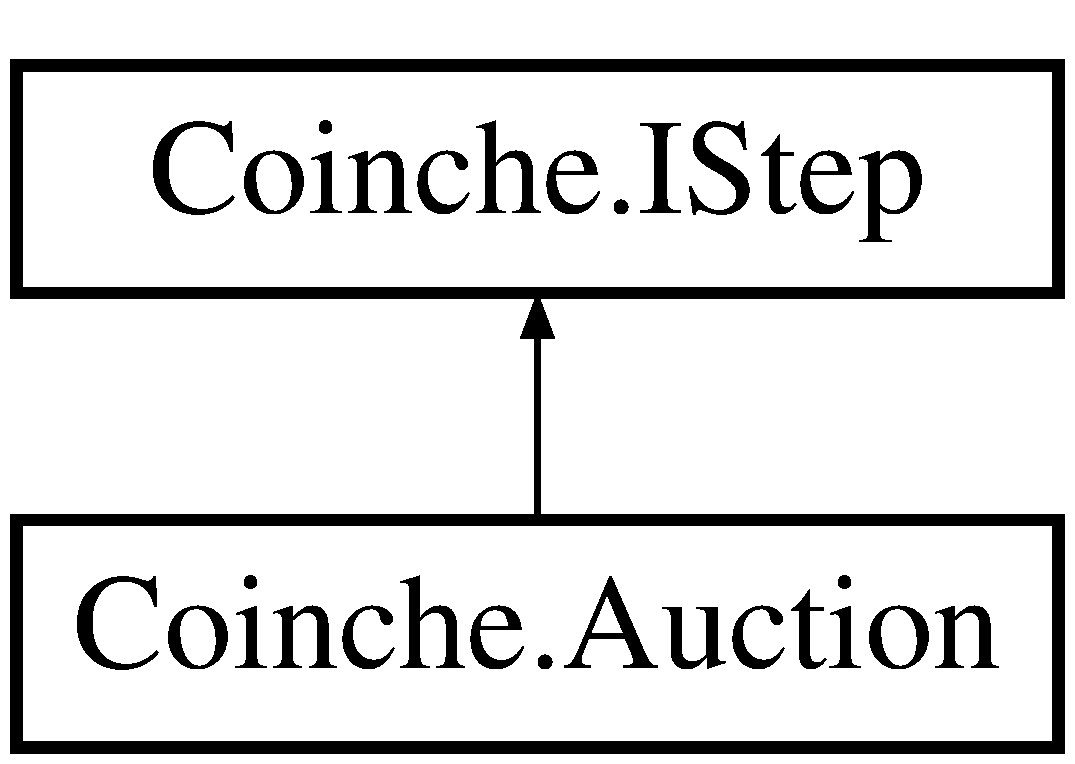
\includegraphics[height=2.000000cm]{class_coinche_1_1_auction}
\end{center}
\end{figure}
\subsection*{Private Member Functions}
\begin{DoxyCompactItemize}
\item 
void I\+Step. \hyperlink{class_coinche_1_1_auction_ae6b090721adfc333705f5f79ca9b462a}{Reset} ()
\begin{DoxyCompactList}\small\item\em reset the step \end{DoxyCompactList}\item 
\hyperlink{class_coinche_1_1_tools_1_1_game_info}{Game\+Info} I\+Step. \hyperlink{class_coinche_1_1_auction_a9596ae8ce46f848244854d59c9bedadb}{Prepare\+Step} (\hyperlink{class_coinche_1_1_player}{Player} player, int \hyperlink{class_coinche_1_1_auction_af83095f623b0dd43fa3b3008a1743926}{team\+Contract})
\begin{DoxyCompactList}\small\item\em prepare the players for the next step \end{DoxyCompactList}\item 
\hyperlink{class_coinche_1_1_tools_1_1_game_info}{Game\+Info} I\+Step. \hyperlink{class_coinche_1_1_auction_ac43279f6867bd7896aee8e6ae504c472}{Do\+Step} (\hyperlink{class_coinche_1_1_player}{Player} player, string msg, Boolean all\+Assets, Boolean none\+Assets, Card\+Color colore\+Bet, int first\+Player)
\begin{DoxyCompactList}\small\item\em rules of the current step applied with the players messages \end{DoxyCompactList}\item 
\mbox{\Hypertarget{class_coinche_1_1_auction_a4d26a9a7fbe7ef886c75d8393750ab9b}\label{class_coinche_1_1_auction_a4d26a9a7fbe7ef886c75d8393750ab9b}} 
string \mbox{[}$\,$\mbox{]} {\bfseries Is\+Invalid\+Bet} (string bet)
\item 
\hyperlink{class_coinche_1_1_tools_1_1_game_info}{Game\+Info} I\+Step. \hyperlink{class_coinche_1_1_auction_a00eba97a2289eb3bf7b2f4f7c84c8349}{Invalid\+Turn} (\hyperlink{class_coinche_1_1_player}{Player} player)
\begin{DoxyCompactList}\small\item\em function called if it wasn\textquotesingle{}t the right turn to play \end{DoxyCompactList}\item 
string I\+Step. \hyperlink{class_coinche_1_1_auction_ab1621fd742e17a9814671116d4d0682c}{Step\+Over} ()
\begin{DoxyCompactList}\small\item\em function called when the step is over \end{DoxyCompactList}\item 
\mbox{\Hypertarget{class_coinche_1_1_auction_a735cc73557e52573a0869a34d155f301}\label{class_coinche_1_1_auction_a735cc73557e52573a0869a34d155f301}} 
string {\bfseries Bet\+Status} ()
\item 
\mbox{\Hypertarget{class_coinche_1_1_auction_aa5d49df07ba1d4548544b0c8caafe687}\label{class_coinche_1_1_auction_aa5d49df07ba1d4548544b0c8caafe687}} 
Boolean {\bfseries Everybody\+Skipped} ()
\end{DoxyCompactItemize}
\subsection*{Private Attributes}
\begin{DoxyCompactItemize}
\item 
string \mbox{[}$\,$\mbox{]} \hyperlink{class_coinche_1_1_auction_a4f6d5c63987543272a3f34676c23970e}{bets}
\begin{DoxyCompactList}\small\item\em Variables needed when defining the contract \end{DoxyCompactList}\item 
\mbox{\Hypertarget{class_coinche_1_1_auction_a929f882e7bca1c896b2fd7c7f02f93c4}\label{class_coinche_1_1_auction_a929f882e7bca1c896b2fd7c7f02f93c4}} 
string {\bfseries best\+Bet}
\item 
\mbox{\Hypertarget{class_coinche_1_1_auction_a9d2f45abe3188b340099fa308641b906}\label{class_coinche_1_1_auction_a9d2f45abe3188b340099fa308641b906}} 
int {\bfseries last\+Player\+Who\+Bet}
\item 
int \hyperlink{class_coinche_1_1_auction_af83095f623b0dd43fa3b3008a1743926}{team\+Contract}
\begin{DoxyCompactList}\small\item\em Variables defining the final contract \end{DoxyCompactList}\item 
\mbox{\Hypertarget{class_coinche_1_1_auction_ad3b33032c91edf13209e109602372bbc}\label{class_coinche_1_1_auction_ad3b33032c91edf13209e109602372bbc}} 
int {\bfseries points\+Bet}
\item 
\mbox{\Hypertarget{class_coinche_1_1_auction_a147a2d497ce78f73fcec3057ef9cc2a8}\label{class_coinche_1_1_auction_a147a2d497ce78f73fcec3057ef9cc2a8}} 
Card\+Color {\bfseries color\+Bet}
\item 
\mbox{\Hypertarget{class_coinche_1_1_auction_af155ec175f8fcccc9ffd106948bea164}\label{class_coinche_1_1_auction_af155ec175f8fcccc9ffd106948bea164}} 
Boolean {\bfseries all\+Assets}
\item 
\mbox{\Hypertarget{class_coinche_1_1_auction_a344dc87f31b624e98aa58552f8679b36}\label{class_coinche_1_1_auction_a344dc87f31b624e98aa58552f8679b36}} 
Boolean {\bfseries none\+Assets}
\end{DoxyCompactItemize}
\subsection*{Additional Inherited Members}


\subsection{Member Function Documentation}
\mbox{\Hypertarget{class_coinche_1_1_auction_ac43279f6867bd7896aee8e6ae504c472}\label{class_coinche_1_1_auction_ac43279f6867bd7896aee8e6ae504c472}} 
\index{Coinche\+::\+Auction@{Coinche\+::\+Auction}!Do\+Step@{Do\+Step}}
\index{Do\+Step@{Do\+Step}!Coinche\+::\+Auction@{Coinche\+::\+Auction}}
\subsubsection{\texorpdfstring{Do\+Step()}{DoStep()}}
{\footnotesize\ttfamily \hyperlink{class_coinche_1_1_tools_1_1_game_info}{Game\+Info} I\+Step. Coinche.\+Auction.\+Do\+Step (\begin{DoxyParamCaption}\item[{\hyperlink{class_coinche_1_1_player}{Player}}]{player,  }\item[{string}]{msg,  }\item[{Boolean}]{all\+Assets,  }\item[{Boolean}]{none\+Assets,  }\item[{Card\+Color}]{colore\+Bet,  }\item[{int}]{first\+Player }\end{DoxyParamCaption})\hspace{0.3cm}{\ttfamily [inline]}, {\ttfamily [private]}}



rules of the current step applied with the players messages 


\begin{DoxyParams}{Parameters}
{\em player} & \\
\hline
{\em msg} & \\
\hline
{\em all\+Assets} & \\
\hline
{\em none\+Assets} & \\
\hline
{\em colore\+Bet} & \\
\hline
{\em first\+Player} & \\
\hline
\end{DoxyParams}
\begin{DoxyReturn}{Returns}
a Game\+Info instance to tell players what happened
\end{DoxyReturn}


Implements \hyperlink{interface_coinche_1_1_i_step_a1b410159a7988ae4e75154539715e7ba}{Coinche.\+I\+Step}.

\mbox{\Hypertarget{class_coinche_1_1_auction_a00eba97a2289eb3bf7b2f4f7c84c8349}\label{class_coinche_1_1_auction_a00eba97a2289eb3bf7b2f4f7c84c8349}} 
\index{Coinche\+::\+Auction@{Coinche\+::\+Auction}!Invalid\+Turn@{Invalid\+Turn}}
\index{Invalid\+Turn@{Invalid\+Turn}!Coinche\+::\+Auction@{Coinche\+::\+Auction}}
\subsubsection{\texorpdfstring{Invalid\+Turn()}{InvalidTurn()}}
{\footnotesize\ttfamily \hyperlink{class_coinche_1_1_tools_1_1_game_info}{Game\+Info} I\+Step. Coinche.\+Auction.\+Invalid\+Turn (\begin{DoxyParamCaption}\item[{\hyperlink{class_coinche_1_1_player}{Player}}]{player }\end{DoxyParamCaption})\hspace{0.3cm}{\ttfamily [inline]}, {\ttfamily [private]}}



function called if it wasn\textquotesingle{}t the right turn to play 


\begin{DoxyParams}{Parameters}
{\em player} & \\
\hline
\end{DoxyParams}
\begin{DoxyReturn}{Returns}
a Game\+Info instance to inform the player it wasn\textquotesingle{}t his turn to play
\end{DoxyReturn}


Implements \hyperlink{interface_coinche_1_1_i_step_afc64813670860f5ee0829264751abc0a}{Coinche.\+I\+Step}.

\mbox{\Hypertarget{class_coinche_1_1_auction_a9596ae8ce46f848244854d59c9bedadb}\label{class_coinche_1_1_auction_a9596ae8ce46f848244854d59c9bedadb}} 
\index{Coinche\+::\+Auction@{Coinche\+::\+Auction}!Prepare\+Step@{Prepare\+Step}}
\index{Prepare\+Step@{Prepare\+Step}!Coinche\+::\+Auction@{Coinche\+::\+Auction}}
\subsubsection{\texorpdfstring{Prepare\+Step()}{PrepareStep()}}
{\footnotesize\ttfamily \hyperlink{class_coinche_1_1_tools_1_1_game_info}{Game\+Info} I\+Step. Coinche.\+Auction.\+Prepare\+Step (\begin{DoxyParamCaption}\item[{\hyperlink{class_coinche_1_1_player}{Player}}]{player,  }\item[{int}]{team\+Contract }\end{DoxyParamCaption})\hspace{0.3cm}{\ttfamily [inline]}, {\ttfamily [private]}}



prepare the players for the next step 


\begin{DoxyParams}{Parameters}
{\em player} & \\
\hline
{\em team\+Contract} & \\
\hline
\end{DoxyParams}
\begin{DoxyReturn}{Returns}
infos to tell them what to do
\end{DoxyReturn}


Implements \hyperlink{interface_coinche_1_1_i_step_ada17a0e471c5afbc7e4f4acc434cdd76}{Coinche.\+I\+Step}.

\mbox{\Hypertarget{class_coinche_1_1_auction_ae6b090721adfc333705f5f79ca9b462a}\label{class_coinche_1_1_auction_ae6b090721adfc333705f5f79ca9b462a}} 
\index{Coinche\+::\+Auction@{Coinche\+::\+Auction}!Reset@{Reset}}
\index{Reset@{Reset}!Coinche\+::\+Auction@{Coinche\+::\+Auction}}
\subsubsection{\texorpdfstring{Reset()}{Reset()}}
{\footnotesize\ttfamily void I\+Step. Coinche.\+Auction.\+Reset (\begin{DoxyParamCaption}{ }\end{DoxyParamCaption})\hspace{0.3cm}{\ttfamily [inline]}, {\ttfamily [private]}}



reset the step 



Implements \hyperlink{interface_coinche_1_1_i_step_a764f20494a35e9b006c6495a38717e9a}{Coinche.\+I\+Step}.

\mbox{\Hypertarget{class_coinche_1_1_auction_ab1621fd742e17a9814671116d4d0682c}\label{class_coinche_1_1_auction_ab1621fd742e17a9814671116d4d0682c}} 
\index{Coinche\+::\+Auction@{Coinche\+::\+Auction}!Step\+Over@{Step\+Over}}
\index{Step\+Over@{Step\+Over}!Coinche\+::\+Auction@{Coinche\+::\+Auction}}
\subsubsection{\texorpdfstring{Step\+Over()}{StepOver()}}
{\footnotesize\ttfamily string I\+Step. Coinche.\+Auction.\+Step\+Over (\begin{DoxyParamCaption}{ }\end{DoxyParamCaption})\hspace{0.3cm}{\ttfamily [inline]}, {\ttfamily [private]}}



function called when the step is over 

\begin{DoxyReturn}{Returns}
a string to tell players the step is over
\end{DoxyReturn}


Implements \hyperlink{interface_coinche_1_1_i_step_a86ef55b4c36ffa27f5fa18a10e9a61a0}{Coinche.\+I\+Step}.



\subsection{Member Data Documentation}
\mbox{\Hypertarget{class_coinche_1_1_auction_a4f6d5c63987543272a3f34676c23970e}\label{class_coinche_1_1_auction_a4f6d5c63987543272a3f34676c23970e}} 
\index{Coinche\+::\+Auction@{Coinche\+::\+Auction}!bets@{bets}}
\index{bets@{bets}!Coinche\+::\+Auction@{Coinche\+::\+Auction}}
\subsubsection{\texorpdfstring{bets}{bets}}
{\footnotesize\ttfamily string \mbox{[}$\,$\mbox{]} Coinche.\+Auction.\+bets\hspace{0.3cm}{\ttfamily [private]}}



Variables needed when defining the contract 

\mbox{\Hypertarget{class_coinche_1_1_auction_af83095f623b0dd43fa3b3008a1743926}\label{class_coinche_1_1_auction_af83095f623b0dd43fa3b3008a1743926}} 
\index{Coinche\+::\+Auction@{Coinche\+::\+Auction}!team\+Contract@{team\+Contract}}
\index{team\+Contract@{team\+Contract}!Coinche\+::\+Auction@{Coinche\+::\+Auction}}
\subsubsection{\texorpdfstring{team\+Contract}{teamContract}}
{\footnotesize\ttfamily int Coinche.\+Auction.\+team\+Contract\hspace{0.3cm}{\ttfamily [private]}}



Variables defining the final contract 



The documentation for this class was generated from the following file\+:\begin{DoxyCompactItemize}
\item 
Server/\+Game\+Rules/\+Steps/\+Auction/Auction.\+cs\end{DoxyCompactItemize}

\hypertarget{class_coinche_1_1_board}{}\section{Coinche.\+Board Class Reference}
\label{class_coinche_1_1_board}\index{Coinche.\+Board@{Coinche.\+Board}}


class representing the board  


\subsection*{Public Member Functions}
\begin{DoxyCompactItemize}
\item 
\hyperlink{class_coinche_1_1_board_a62235716a2f4c7726973aca20cd46fce}{Board} ()
\begin{DoxyCompactList}\small\item\em simple constructor \end{DoxyCompactList}\item 
void \hyperlink{class_coinche_1_1_board_a5c17c44b33d20c90868cad3b504c4ae4}{Reset} ()
\begin{DoxyCompactList}\small\item\em clear the board \end{DoxyCompactList}\item 
string \hyperlink{class_coinche_1_1_board_ae95210444e9e18af75f0b55827842905}{Board\+Status} ()
\begin{DoxyCompactList}\small\item\em get the board status as a string \end{DoxyCompactList}\item 
Boolean \hyperlink{class_coinche_1_1_board_a9f83f16052be20631b1645edd53d8adb}{Is\+Full} ()
\begin{DoxyCompactList}\small\item\em check if the board is full \end{DoxyCompactList}\end{DoxyCompactItemize}
\subsection*{Properties}
\begin{DoxyCompactItemize}
\item 
\hyperlink{class_coinche_1_1_card}{Card} \mbox{[}$\,$\mbox{]} \hyperlink{class_coinche_1_1_board_a06fcff9cacac2e531c446007cece8751}{Cards\+Played}\hspace{0.3cm}{\ttfamily  \mbox{[}get, set\mbox{]}}
\begin{DoxyCompactList}\small\item\em array of the cards on the board (null if there is no card) \end{DoxyCompactList}\end{DoxyCompactItemize}


\subsection{Detailed Description}
class representing the board 



\subsection{Constructor \& Destructor Documentation}
\mbox{\Hypertarget{class_coinche_1_1_board_a62235716a2f4c7726973aca20cd46fce}\label{class_coinche_1_1_board_a62235716a2f4c7726973aca20cd46fce}} 
\index{Coinche\+::\+Board@{Coinche\+::\+Board}!Board@{Board}}
\index{Board@{Board}!Coinche\+::\+Board@{Coinche\+::\+Board}}
\subsubsection{\texorpdfstring{Board()}{Board()}}
{\footnotesize\ttfamily Coinche.\+Board.\+Board (\begin{DoxyParamCaption}{ }\end{DoxyParamCaption})\hspace{0.3cm}{\ttfamily [inline]}}



simple constructor 



\subsection{Member Function Documentation}
\mbox{\Hypertarget{class_coinche_1_1_board_ae95210444e9e18af75f0b55827842905}\label{class_coinche_1_1_board_ae95210444e9e18af75f0b55827842905}} 
\index{Coinche\+::\+Board@{Coinche\+::\+Board}!Board\+Status@{Board\+Status}}
\index{Board\+Status@{Board\+Status}!Coinche\+::\+Board@{Coinche\+::\+Board}}
\subsubsection{\texorpdfstring{Board\+Status()}{BoardStatus()}}
{\footnotesize\ttfamily string Coinche.\+Board.\+Board\+Status (\begin{DoxyParamCaption}{ }\end{DoxyParamCaption})\hspace{0.3cm}{\ttfamily [inline]}}



get the board status as a string 

\begin{DoxyReturn}{Returns}
the cards on the board
\end{DoxyReturn}
\mbox{\Hypertarget{class_coinche_1_1_board_a9f83f16052be20631b1645edd53d8adb}\label{class_coinche_1_1_board_a9f83f16052be20631b1645edd53d8adb}} 
\index{Coinche\+::\+Board@{Coinche\+::\+Board}!Is\+Full@{Is\+Full}}
\index{Is\+Full@{Is\+Full}!Coinche\+::\+Board@{Coinche\+::\+Board}}
\subsubsection{\texorpdfstring{Is\+Full()}{IsFull()}}
{\footnotesize\ttfamily Boolean Coinche.\+Board.\+Is\+Full (\begin{DoxyParamCaption}{ }\end{DoxyParamCaption})\hspace{0.3cm}{\ttfamily [inline]}}



check if the board is full 

\begin{DoxyReturn}{Returns}
true if its full else false
\end{DoxyReturn}
\mbox{\Hypertarget{class_coinche_1_1_board_a5c17c44b33d20c90868cad3b504c4ae4}\label{class_coinche_1_1_board_a5c17c44b33d20c90868cad3b504c4ae4}} 
\index{Coinche\+::\+Board@{Coinche\+::\+Board}!Reset@{Reset}}
\index{Reset@{Reset}!Coinche\+::\+Board@{Coinche\+::\+Board}}
\subsubsection{\texorpdfstring{Reset()}{Reset()}}
{\footnotesize\ttfamily void Coinche.\+Board.\+Reset (\begin{DoxyParamCaption}{ }\end{DoxyParamCaption})\hspace{0.3cm}{\ttfamily [inline]}}



clear the board 



\subsection{Property Documentation}
\mbox{\Hypertarget{class_coinche_1_1_board_a06fcff9cacac2e531c446007cece8751}\label{class_coinche_1_1_board_a06fcff9cacac2e531c446007cece8751}} 
\index{Coinche\+::\+Board@{Coinche\+::\+Board}!Cards\+Played@{Cards\+Played}}
\index{Cards\+Played@{Cards\+Played}!Coinche\+::\+Board@{Coinche\+::\+Board}}
\subsubsection{\texorpdfstring{Cards\+Played}{CardsPlayed}}
{\footnotesize\ttfamily \hyperlink{class_coinche_1_1_card}{Card} \mbox{[}$\,$\mbox{]} Coinche.\+Board.\+Cards\+Played\hspace{0.3cm}{\ttfamily [get]}, {\ttfamily [set]}}



array of the cards on the board (null if there is no card) 



The documentation for this class was generated from the following file\+:\begin{DoxyCompactItemize}
\item 
Server/\+Game\+Rules/Board.\+cs\end{DoxyCompactItemize}

\hypertarget{class_coinche_1_1_card}{}\section{Coinche.\+Card Class Reference}
\label{class_coinche_1_1_card}\index{Coinche.\+Card@{Coinche.\+Card}}


class defining a card  


\subsection*{Public Member Functions}
\begin{DoxyCompactItemize}
\item 
\hyperlink{class_coinche_1_1_card_a9605eece142f74828e18131057a3d180}{Card} (Card\+Color c, Card\+Value v)
\begin{DoxyCompactList}\small\item\em Basic constructor that initialize a card \end{DoxyCompactList}\end{DoxyCompactItemize}
\subsection*{Properties}
\begin{DoxyCompactItemize}
\item 
Card\+Color \hyperlink{class_coinche_1_1_card_aa16b6cca19c354b8243cae302c1ef7ef}{Color}\hspace{0.3cm}{\ttfamily  \mbox{[}get\mbox{]}}
\begin{DoxyCompactList}\small\item\em color of the card \end{DoxyCompactList}\item 
Card\+Value \hyperlink{class_coinche_1_1_card_a78224b5558f9f9bbd4036be50f4da865}{Value}\hspace{0.3cm}{\ttfamily  \mbox{[}get\mbox{]}}
\begin{DoxyCompactList}\small\item\em value of the card \end{DoxyCompactList}\item 
int \hyperlink{class_coinche_1_1_card_a554cc67985a48ffafe912e35f725c898}{Power\+Asset}\hspace{0.3cm}{\ttfamily  \mbox{[}get\mbox{]}}
\begin{DoxyCompactList}\small\item\em power of the card if its color is the asset one \end{DoxyCompactList}\item 
int \hyperlink{class_coinche_1_1_card_a1bdf34d04e55d97bcf2163b811c78dd3}{Power\+Non\+Asset}\hspace{0.3cm}{\ttfamily  \mbox{[}get\mbox{]}}
\begin{DoxyCompactList}\small\item\em power of the card if it\textquotesingle{}s not an asset \end{DoxyCompactList}\item 
int \hyperlink{class_coinche_1_1_card_ae6c4c19d3fb112f06eceb9b9b67ad9d6}{Points\+Asset}\hspace{0.3cm}{\ttfamily  \mbox{[}get\mbox{]}}
\begin{DoxyCompactList}\small\item\em points of the card if it\textquotesingle{}s an asset \end{DoxyCompactList}\item 
int \hyperlink{class_coinche_1_1_card_a2f5e7d69b5492f3af0b738b2bb3013e4}{Points\+Non\+Asset}\hspace{0.3cm}{\ttfamily  \mbox{[}get\mbox{]}}
\begin{DoxyCompactList}\small\item\em points of the card if it\textquotesingle{}s not an asset \end{DoxyCompactList}\item 
int \hyperlink{class_coinche_1_1_card_ad9c940b967ccd302b1f210fa07c09315}{Points\+All\+Assets}\hspace{0.3cm}{\ttfamily  \mbox{[}get\mbox{]}}
\begin{DoxyCompactList}\small\item\em points of the card if all cards are assets \end{DoxyCompactList}\item 
int \hyperlink{class_coinche_1_1_card_ac33c19e7a4f0a5fd3112daed9266bf6c}{Points\+None\+Assets}\hspace{0.3cm}{\ttfamily  \mbox{[}get\mbox{]}}
\begin{DoxyCompactList}\small\item\em points of the card if there is none assets \end{DoxyCompactList}\end{DoxyCompactItemize}


\subsection{Detailed Description}
class defining a card 



\subsection{Constructor \& Destructor Documentation}
\mbox{\Hypertarget{class_coinche_1_1_card_a9605eece142f74828e18131057a3d180}\label{class_coinche_1_1_card_a9605eece142f74828e18131057a3d180}} 
\index{Coinche\+::\+Card@{Coinche\+::\+Card}!Card@{Card}}
\index{Card@{Card}!Coinche\+::\+Card@{Coinche\+::\+Card}}
\subsubsection{\texorpdfstring{Card()}{Card()}}
{\footnotesize\ttfamily Coinche.\+Card.\+Card (\begin{DoxyParamCaption}\item[{Card\+Color}]{c,  }\item[{Card\+Value}]{v }\end{DoxyParamCaption})\hspace{0.3cm}{\ttfamily [inline]}}



Basic constructor that initialize a card 



\subsection{Property Documentation}
\mbox{\Hypertarget{class_coinche_1_1_card_aa16b6cca19c354b8243cae302c1ef7ef}\label{class_coinche_1_1_card_aa16b6cca19c354b8243cae302c1ef7ef}} 
\index{Coinche\+::\+Card@{Coinche\+::\+Card}!Color@{Color}}
\index{Color@{Color}!Coinche\+::\+Card@{Coinche\+::\+Card}}
\subsubsection{\texorpdfstring{Color}{Color}}
{\footnotesize\ttfamily Card\+Color Coinche.\+Card.\+Color\hspace{0.3cm}{\ttfamily [get]}}



color of the card 

\mbox{\Hypertarget{class_coinche_1_1_card_ad9c940b967ccd302b1f210fa07c09315}\label{class_coinche_1_1_card_ad9c940b967ccd302b1f210fa07c09315}} 
\index{Coinche\+::\+Card@{Coinche\+::\+Card}!Points\+All\+Assets@{Points\+All\+Assets}}
\index{Points\+All\+Assets@{Points\+All\+Assets}!Coinche\+::\+Card@{Coinche\+::\+Card}}
\subsubsection{\texorpdfstring{Points\+All\+Assets}{PointsAllAssets}}
{\footnotesize\ttfamily int Coinche.\+Card.\+Points\+All\+Assets\hspace{0.3cm}{\ttfamily [get]}}



points of the card if all cards are assets 

\mbox{\Hypertarget{class_coinche_1_1_card_ae6c4c19d3fb112f06eceb9b9b67ad9d6}\label{class_coinche_1_1_card_ae6c4c19d3fb112f06eceb9b9b67ad9d6}} 
\index{Coinche\+::\+Card@{Coinche\+::\+Card}!Points\+Asset@{Points\+Asset}}
\index{Points\+Asset@{Points\+Asset}!Coinche\+::\+Card@{Coinche\+::\+Card}}
\subsubsection{\texorpdfstring{Points\+Asset}{PointsAsset}}
{\footnotesize\ttfamily int Coinche.\+Card.\+Points\+Asset\hspace{0.3cm}{\ttfamily [get]}}



points of the card if it\textquotesingle{}s an asset 

\mbox{\Hypertarget{class_coinche_1_1_card_a2f5e7d69b5492f3af0b738b2bb3013e4}\label{class_coinche_1_1_card_a2f5e7d69b5492f3af0b738b2bb3013e4}} 
\index{Coinche\+::\+Card@{Coinche\+::\+Card}!Points\+Non\+Asset@{Points\+Non\+Asset}}
\index{Points\+Non\+Asset@{Points\+Non\+Asset}!Coinche\+::\+Card@{Coinche\+::\+Card}}
\subsubsection{\texorpdfstring{Points\+Non\+Asset}{PointsNonAsset}}
{\footnotesize\ttfamily int Coinche.\+Card.\+Points\+Non\+Asset\hspace{0.3cm}{\ttfamily [get]}}



points of the card if it\textquotesingle{}s not an asset 

\mbox{\Hypertarget{class_coinche_1_1_card_ac33c19e7a4f0a5fd3112daed9266bf6c}\label{class_coinche_1_1_card_ac33c19e7a4f0a5fd3112daed9266bf6c}} 
\index{Coinche\+::\+Card@{Coinche\+::\+Card}!Points\+None\+Assets@{Points\+None\+Assets}}
\index{Points\+None\+Assets@{Points\+None\+Assets}!Coinche\+::\+Card@{Coinche\+::\+Card}}
\subsubsection{\texorpdfstring{Points\+None\+Assets}{PointsNoneAssets}}
{\footnotesize\ttfamily int Coinche.\+Card.\+Points\+None\+Assets\hspace{0.3cm}{\ttfamily [get]}}



points of the card if there is none assets 

\mbox{\Hypertarget{class_coinche_1_1_card_a554cc67985a48ffafe912e35f725c898}\label{class_coinche_1_1_card_a554cc67985a48ffafe912e35f725c898}} 
\index{Coinche\+::\+Card@{Coinche\+::\+Card}!Power\+Asset@{Power\+Asset}}
\index{Power\+Asset@{Power\+Asset}!Coinche\+::\+Card@{Coinche\+::\+Card}}
\subsubsection{\texorpdfstring{Power\+Asset}{PowerAsset}}
{\footnotesize\ttfamily int Coinche.\+Card.\+Power\+Asset\hspace{0.3cm}{\ttfamily [get]}}



power of the card if its color is the asset one 

\mbox{\Hypertarget{class_coinche_1_1_card_a1bdf34d04e55d97bcf2163b811c78dd3}\label{class_coinche_1_1_card_a1bdf34d04e55d97bcf2163b811c78dd3}} 
\index{Coinche\+::\+Card@{Coinche\+::\+Card}!Power\+Non\+Asset@{Power\+Non\+Asset}}
\index{Power\+Non\+Asset@{Power\+Non\+Asset}!Coinche\+::\+Card@{Coinche\+::\+Card}}
\subsubsection{\texorpdfstring{Power\+Non\+Asset}{PowerNonAsset}}
{\footnotesize\ttfamily int Coinche.\+Card.\+Power\+Non\+Asset\hspace{0.3cm}{\ttfamily [get]}}



power of the card if it\textquotesingle{}s not an asset 

\mbox{\Hypertarget{class_coinche_1_1_card_a78224b5558f9f9bbd4036be50f4da865}\label{class_coinche_1_1_card_a78224b5558f9f9bbd4036be50f4da865}} 
\index{Coinche\+::\+Card@{Coinche\+::\+Card}!Value@{Value}}
\index{Value@{Value}!Coinche\+::\+Card@{Coinche\+::\+Card}}
\subsubsection{\texorpdfstring{Value}{Value}}
{\footnotesize\ttfamily Card\+Value Coinche.\+Card.\+Value\hspace{0.3cm}{\ttfamily [get]}}



value of the card 



The documentation for this class was generated from the following file\+:\begin{DoxyCompactItemize}
\item 
Server/\+Game\+Rules/Card.\+cs\end{DoxyCompactItemize}

\hypertarget{class_coinche_1_1_google_1_1_protobuf_1_1_coinche_protocol_reflection}{}\section{Coinche.\+Google.\+Protobuf.\+Coinche\+Protocol\+Reflection Class Reference}
\label{class_coinche_1_1_google_1_1_protobuf_1_1_coinche_protocol_reflection}\index{Coinche.\+Google.\+Protobuf.\+Coinche\+Protocol\+Reflection@{Coinche.\+Google.\+Protobuf.\+Coinche\+Protocol\+Reflection}}


Holder for reflection information generated from Coinche\+Protocol.\+proto 


\subsection*{Properties}
\begin{DoxyCompactItemize}
\item 
static pbr\+::\+File\+Descriptor \hyperlink{class_coinche_1_1_google_1_1_protobuf_1_1_coinche_protocol_reflection_a6ec0abfdc3d27a45c490e69e185dbfdd}{Descriptor}\hspace{0.3cm}{\ttfamily  \mbox{[}get\mbox{]}}
\begin{DoxyCompactList}\small\item\em File descriptor for Coinche\+Protocol.\+proto\end{DoxyCompactList}\end{DoxyCompactItemize}
\subsection*{Static Private Attributes}
\begin{DoxyCompactItemize}
\item 
\mbox{\Hypertarget{class_coinche_1_1_google_1_1_protobuf_1_1_coinche_protocol_reflection_aa196d460ba1df0e1be672777ad6fb1e7}\label{class_coinche_1_1_google_1_1_protobuf_1_1_coinche_protocol_reflection_aa196d460ba1df0e1be672777ad6fb1e7}} 
static pbr\+::\+File\+Descriptor {\bfseries descriptor}
\end{DoxyCompactItemize}


\subsection{Detailed Description}
Holder for reflection information generated from Coinche\+Protocol.\+proto



\subsection{Property Documentation}
\mbox{\Hypertarget{class_coinche_1_1_google_1_1_protobuf_1_1_coinche_protocol_reflection_a6ec0abfdc3d27a45c490e69e185dbfdd}\label{class_coinche_1_1_google_1_1_protobuf_1_1_coinche_protocol_reflection_a6ec0abfdc3d27a45c490e69e185dbfdd}} 
\index{Coinche\+::\+Google\+::\+Protobuf\+::\+Coinche\+Protocol\+Reflection@{Coinche\+::\+Google\+::\+Protobuf\+::\+Coinche\+Protocol\+Reflection}!Descriptor@{Descriptor}}
\index{Descriptor@{Descriptor}!Coinche\+::\+Google\+::\+Protobuf\+::\+Coinche\+Protocol\+Reflection@{Coinche\+::\+Google\+::\+Protobuf\+::\+Coinche\+Protocol\+Reflection}}
\subsubsection{\texorpdfstring{Descriptor}{Descriptor}}
{\footnotesize\ttfamily static pbr.\+File\+Descriptor Coinche.\+Google.\+Protobuf.\+Coinche\+Protocol\+Reflection.\+Descriptor\hspace{0.3cm}{\ttfamily [static]}, {\ttfamily [get]}}



File descriptor for Coinche\+Protocol.\+proto



The documentation for this class was generated from the following file\+:\begin{DoxyCompactItemize}
\item 
Client/\+Protobuf/Coinche\+Protocol.\+cs\end{DoxyCompactItemize}

\hypertarget{class_server_1_1_game_rules_1_1_steps_1_1_counter_1_1_counter}{}\section{Server.\+Game\+Rules.\+Steps.\+Counter.\+Counter Class Reference}
\label{class_server_1_1_game_rules_1_1_steps_1_1_counter_1_1_counter}\index{Server.\+Game\+Rules.\+Steps.\+Counter.\+Counter@{Server.\+Game\+Rules.\+Steps.\+Counter.\+Counter}}


class representing the tricks step  


Inheritance diagram for Server.\+Game\+Rules.\+Steps.\+Counter.\+Counter\+:\begin{figure}[H]
\begin{center}
\leavevmode
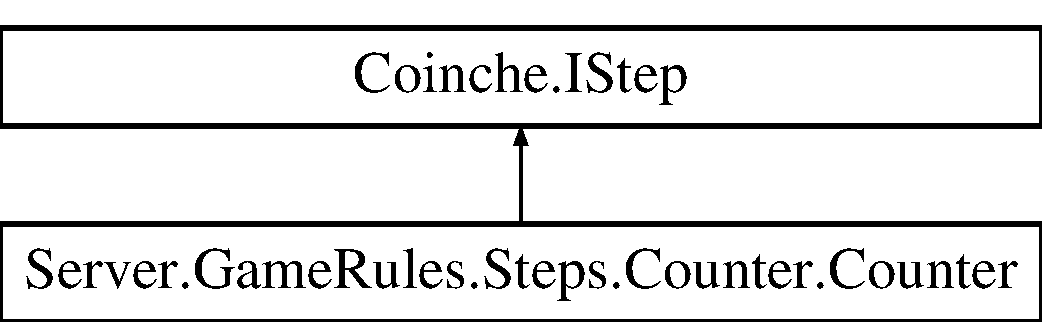
\includegraphics[height=2.000000cm]{class_server_1_1_game_rules_1_1_steps_1_1_counter_1_1_counter}
\end{center}
\end{figure}
\subsection*{Private Member Functions}
\begin{DoxyCompactItemize}
\item 
void I\+Step. \hyperlink{class_server_1_1_game_rules_1_1_steps_1_1_counter_1_1_counter_a7e681c51f20d2509e0b53dede3d73dc0}{Reset} ()
\begin{DoxyCompactList}\small\item\em reset the step \end{DoxyCompactList}\item 
\hyperlink{class_coinche_1_1_tools_1_1_game_info}{Game\+Info} I\+Step. \hyperlink{class_server_1_1_game_rules_1_1_steps_1_1_counter_1_1_counter_a84412648384fce7fea870e5e1e32bc3d}{Prepare\+Step} (\hyperlink{class_coinche_1_1_player}{Player} player, int team\+Contract)
\begin{DoxyCompactList}\small\item\em prepare the players for the next step \end{DoxyCompactList}\item 
\hyperlink{class_coinche_1_1_tools_1_1_game_info}{Game\+Info} I\+Step. \hyperlink{class_server_1_1_game_rules_1_1_steps_1_1_counter_1_1_counter_aba717018db3366659fdb4ac302d19937}{Do\+Step} (\hyperlink{class_coinche_1_1_player}{Player} player, string msg, Boolean all\+Assets, Boolean none\+Assets, Card\+Color color\+Bet, int first\+Player)
\begin{DoxyCompactList}\small\item\em rules of the current step applied with the players messages \end{DoxyCompactList}\item 
\hyperlink{class_coinche_1_1_tools_1_1_game_info}{Game\+Info} I\+Step. \hyperlink{class_server_1_1_game_rules_1_1_steps_1_1_counter_1_1_counter_a81fc65a550bef61081dd1ec351b3bdaf}{Invalid\+Turn} (\hyperlink{class_coinche_1_1_player}{Player} player)
\begin{DoxyCompactList}\small\item\em function called if it wasn\textquotesingle{}t the right turn to play \end{DoxyCompactList}\item 
string I\+Step. \hyperlink{class_server_1_1_game_rules_1_1_steps_1_1_counter_1_1_counter_a75247ce8610225edadc753a432dd9c56}{Step\+Over} ()
\begin{DoxyCompactList}\small\item\em function called when the step is over \end{DoxyCompactList}\end{DoxyCompactItemize}
\subsection*{Private Attributes}
\begin{DoxyCompactItemize}
\item 
string \hyperlink{class_server_1_1_game_rules_1_1_steps_1_1_counter_1_1_counter_ad8d4f8ccac9f1aff4fe285de35a60f71}{What\+Do\+You\+Want}
\begin{DoxyCompactList}\small\item\em string representing the status of the counter (\hyperlink{namespace_coinche}{Coinche} or Surcoinche) \end{DoxyCompactList}\item 
int \hyperlink{class_server_1_1_game_rules_1_1_steps_1_1_counter_1_1_counter_a073b124596a28a8eebeb1dd4715ed6cf}{mult}
\begin{DoxyCompactList}\small\item\em score multipicator (1, 2 or 4) \end{DoxyCompactList}\end{DoxyCompactItemize}
\subsection*{Additional Inherited Members}


\subsection{Detailed Description}
class representing the tricks step 



\subsection{Member Function Documentation}
\mbox{\Hypertarget{class_server_1_1_game_rules_1_1_steps_1_1_counter_1_1_counter_aba717018db3366659fdb4ac302d19937}\label{class_server_1_1_game_rules_1_1_steps_1_1_counter_1_1_counter_aba717018db3366659fdb4ac302d19937}} 
\index{Server\+::\+Game\+Rules\+::\+Steps\+::\+Counter\+::\+Counter@{Server\+::\+Game\+Rules\+::\+Steps\+::\+Counter\+::\+Counter}!Do\+Step@{Do\+Step}}
\index{Do\+Step@{Do\+Step}!Server\+::\+Game\+Rules\+::\+Steps\+::\+Counter\+::\+Counter@{Server\+::\+Game\+Rules\+::\+Steps\+::\+Counter\+::\+Counter}}
\subsubsection{\texorpdfstring{Do\+Step()}{DoStep()}}
{\footnotesize\ttfamily \hyperlink{class_coinche_1_1_tools_1_1_game_info}{Game\+Info} I\+Step. Server.\+Game\+Rules.\+Steps.\+Counter.\+Counter.\+Do\+Step (\begin{DoxyParamCaption}\item[{\hyperlink{class_coinche_1_1_player}{Player}}]{player,  }\item[{string}]{msg,  }\item[{Boolean}]{all\+Assets,  }\item[{Boolean}]{none\+Assets,  }\item[{Card\+Color}]{color\+Bet,  }\item[{int}]{first\+Player }\end{DoxyParamCaption})\hspace{0.3cm}{\ttfamily [inline]}, {\ttfamily [private]}}



rules of the current step applied with the players messages 


\begin{DoxyParams}{Parameters}
{\em player} & \\
\hline
{\em msg} & \\
\hline
{\em all\+Assets} & \\
\hline
{\em none\+Assets} & \\
\hline
{\em color\+Bet} & \\
\hline
{\em first\+Player} & \\
\hline
\end{DoxyParams}
\begin{DoxyReturn}{Returns}
a Game\+Info instance to tell players what happened
\end{DoxyReturn}


Implements \hyperlink{interface_coinche_1_1_i_step_a1b410159a7988ae4e75154539715e7ba}{Coinche.\+I\+Step}.

\mbox{\Hypertarget{class_server_1_1_game_rules_1_1_steps_1_1_counter_1_1_counter_a81fc65a550bef61081dd1ec351b3bdaf}\label{class_server_1_1_game_rules_1_1_steps_1_1_counter_1_1_counter_a81fc65a550bef61081dd1ec351b3bdaf}} 
\index{Server\+::\+Game\+Rules\+::\+Steps\+::\+Counter\+::\+Counter@{Server\+::\+Game\+Rules\+::\+Steps\+::\+Counter\+::\+Counter}!Invalid\+Turn@{Invalid\+Turn}}
\index{Invalid\+Turn@{Invalid\+Turn}!Server\+::\+Game\+Rules\+::\+Steps\+::\+Counter\+::\+Counter@{Server\+::\+Game\+Rules\+::\+Steps\+::\+Counter\+::\+Counter}}
\subsubsection{\texorpdfstring{Invalid\+Turn()}{InvalidTurn()}}
{\footnotesize\ttfamily \hyperlink{class_coinche_1_1_tools_1_1_game_info}{Game\+Info} I\+Step. Server.\+Game\+Rules.\+Steps.\+Counter.\+Counter.\+Invalid\+Turn (\begin{DoxyParamCaption}\item[{\hyperlink{class_coinche_1_1_player}{Player}}]{player }\end{DoxyParamCaption})\hspace{0.3cm}{\ttfamily [inline]}, {\ttfamily [private]}}



function called if it wasn\textquotesingle{}t the right turn to play 


\begin{DoxyParams}{Parameters}
{\em player} & \\
\hline
\end{DoxyParams}
\begin{DoxyReturn}{Returns}
a Game\+Info instance to inform the player it wasn\textquotesingle{}t his turn to play
\end{DoxyReturn}


Implements \hyperlink{interface_coinche_1_1_i_step_afc64813670860f5ee0829264751abc0a}{Coinche.\+I\+Step}.

\mbox{\Hypertarget{class_server_1_1_game_rules_1_1_steps_1_1_counter_1_1_counter_a84412648384fce7fea870e5e1e32bc3d}\label{class_server_1_1_game_rules_1_1_steps_1_1_counter_1_1_counter_a84412648384fce7fea870e5e1e32bc3d}} 
\index{Server\+::\+Game\+Rules\+::\+Steps\+::\+Counter\+::\+Counter@{Server\+::\+Game\+Rules\+::\+Steps\+::\+Counter\+::\+Counter}!Prepare\+Step@{Prepare\+Step}}
\index{Prepare\+Step@{Prepare\+Step}!Server\+::\+Game\+Rules\+::\+Steps\+::\+Counter\+::\+Counter@{Server\+::\+Game\+Rules\+::\+Steps\+::\+Counter\+::\+Counter}}
\subsubsection{\texorpdfstring{Prepare\+Step()}{PrepareStep()}}
{\footnotesize\ttfamily \hyperlink{class_coinche_1_1_tools_1_1_game_info}{Game\+Info} I\+Step. Server.\+Game\+Rules.\+Steps.\+Counter.\+Counter.\+Prepare\+Step (\begin{DoxyParamCaption}\item[{\hyperlink{class_coinche_1_1_player}{Player}}]{player,  }\item[{int}]{team\+Contract }\end{DoxyParamCaption})\hspace{0.3cm}{\ttfamily [inline]}, {\ttfamily [private]}}



prepare the players for the next step 


\begin{DoxyParams}{Parameters}
{\em player} & \\
\hline
{\em team\+Contract} & \\
\hline
\end{DoxyParams}
\begin{DoxyReturn}{Returns}
infos to tell them what to do
\end{DoxyReturn}


Implements \hyperlink{interface_coinche_1_1_i_step_ada17a0e471c5afbc7e4f4acc434cdd76}{Coinche.\+I\+Step}.

\mbox{\Hypertarget{class_server_1_1_game_rules_1_1_steps_1_1_counter_1_1_counter_a7e681c51f20d2509e0b53dede3d73dc0}\label{class_server_1_1_game_rules_1_1_steps_1_1_counter_1_1_counter_a7e681c51f20d2509e0b53dede3d73dc0}} 
\index{Server\+::\+Game\+Rules\+::\+Steps\+::\+Counter\+::\+Counter@{Server\+::\+Game\+Rules\+::\+Steps\+::\+Counter\+::\+Counter}!Reset@{Reset}}
\index{Reset@{Reset}!Server\+::\+Game\+Rules\+::\+Steps\+::\+Counter\+::\+Counter@{Server\+::\+Game\+Rules\+::\+Steps\+::\+Counter\+::\+Counter}}
\subsubsection{\texorpdfstring{Reset()}{Reset()}}
{\footnotesize\ttfamily void I\+Step. Server.\+Game\+Rules.\+Steps.\+Counter.\+Counter.\+Reset (\begin{DoxyParamCaption}{ }\end{DoxyParamCaption})\hspace{0.3cm}{\ttfamily [inline]}, {\ttfamily [private]}}



reset the step 



Implements \hyperlink{interface_coinche_1_1_i_step_a764f20494a35e9b006c6495a38717e9a}{Coinche.\+I\+Step}.

\mbox{\Hypertarget{class_server_1_1_game_rules_1_1_steps_1_1_counter_1_1_counter_a75247ce8610225edadc753a432dd9c56}\label{class_server_1_1_game_rules_1_1_steps_1_1_counter_1_1_counter_a75247ce8610225edadc753a432dd9c56}} 
\index{Server\+::\+Game\+Rules\+::\+Steps\+::\+Counter\+::\+Counter@{Server\+::\+Game\+Rules\+::\+Steps\+::\+Counter\+::\+Counter}!Step\+Over@{Step\+Over}}
\index{Step\+Over@{Step\+Over}!Server\+::\+Game\+Rules\+::\+Steps\+::\+Counter\+::\+Counter@{Server\+::\+Game\+Rules\+::\+Steps\+::\+Counter\+::\+Counter}}
\subsubsection{\texorpdfstring{Step\+Over()}{StepOver()}}
{\footnotesize\ttfamily string I\+Step. Server.\+Game\+Rules.\+Steps.\+Counter.\+Counter.\+Step\+Over (\begin{DoxyParamCaption}{ }\end{DoxyParamCaption})\hspace{0.3cm}{\ttfamily [inline]}, {\ttfamily [private]}}



function called when the step is over 

\begin{DoxyReturn}{Returns}
a string to tell players the step is over
\end{DoxyReturn}


Implements \hyperlink{interface_coinche_1_1_i_step_a86ef55b4c36ffa27f5fa18a10e9a61a0}{Coinche.\+I\+Step}.



\subsection{Member Data Documentation}
\mbox{\Hypertarget{class_server_1_1_game_rules_1_1_steps_1_1_counter_1_1_counter_a073b124596a28a8eebeb1dd4715ed6cf}\label{class_server_1_1_game_rules_1_1_steps_1_1_counter_1_1_counter_a073b124596a28a8eebeb1dd4715ed6cf}} 
\index{Server\+::\+Game\+Rules\+::\+Steps\+::\+Counter\+::\+Counter@{Server\+::\+Game\+Rules\+::\+Steps\+::\+Counter\+::\+Counter}!mult@{mult}}
\index{mult@{mult}!Server\+::\+Game\+Rules\+::\+Steps\+::\+Counter\+::\+Counter@{Server\+::\+Game\+Rules\+::\+Steps\+::\+Counter\+::\+Counter}}
\subsubsection{\texorpdfstring{mult}{mult}}
{\footnotesize\ttfamily int Server.\+Game\+Rules.\+Steps.\+Counter.\+Counter.\+mult\hspace{0.3cm}{\ttfamily [private]}}



score multipicator (1, 2 or 4) 

\mbox{\Hypertarget{class_server_1_1_game_rules_1_1_steps_1_1_counter_1_1_counter_ad8d4f8ccac9f1aff4fe285de35a60f71}\label{class_server_1_1_game_rules_1_1_steps_1_1_counter_1_1_counter_ad8d4f8ccac9f1aff4fe285de35a60f71}} 
\index{Server\+::\+Game\+Rules\+::\+Steps\+::\+Counter\+::\+Counter@{Server\+::\+Game\+Rules\+::\+Steps\+::\+Counter\+::\+Counter}!What\+Do\+You\+Want@{What\+Do\+You\+Want}}
\index{What\+Do\+You\+Want@{What\+Do\+You\+Want}!Server\+::\+Game\+Rules\+::\+Steps\+::\+Counter\+::\+Counter@{Server\+::\+Game\+Rules\+::\+Steps\+::\+Counter\+::\+Counter}}
\subsubsection{\texorpdfstring{What\+Do\+You\+Want}{WhatDoYouWant}}
{\footnotesize\ttfamily string Server.\+Game\+Rules.\+Steps.\+Counter.\+Counter.\+What\+Do\+You\+Want\hspace{0.3cm}{\ttfamily [private]}}



string representing the status of the counter (\hyperlink{namespace_coinche}{Coinche} or Surcoinche) 



The documentation for this class was generated from the following file\+:\begin{DoxyCompactItemize}
\item 
Server/\+Game\+Rules/\+Steps/\+Counter/Counter.\+cs\end{DoxyCompactItemize}

\hypertarget{class_coinche_1_1_deck}{}\section{Coinche.\+Deck Class Reference}
\label{class_coinche_1_1_deck}\index{Coinche.\+Deck@{Coinche.\+Deck}}


class defining the deck  


\subsection*{Public Member Functions}
\begin{DoxyCompactItemize}
\item 
\hyperlink{class_coinche_1_1_deck_a63fabc6c73f999e4cc1fd55e368f6a30}{Deck} ()
\begin{DoxyCompactList}\small\item\em Basic constructor that creates the deck using the \hyperlink{class_coinche_1_1_card}{Card} class \end{DoxyCompactList}\item 
void \hyperlink{class_coinche_1_1_deck_a2c869fc45763e7c847d51db4016f30a9}{Reset} ()
\begin{DoxyCompactList}\small\item\em Reset the deck state before dealing \end{DoxyCompactList}\item 
void \hyperlink{class_coinche_1_1_deck_a05027ece37a4f59773be023f76c64947}{Display} ()
\begin{DoxyCompactList}\small\item\em Display the cards in the whole deck \end{DoxyCompactList}\item 
void \hyperlink{class_coinche_1_1_deck_a908c7e4a2e22545c903999108b848727}{Shuffle} ()
\begin{DoxyCompactList}\small\item\em Shuffle the deck in a random order \end{DoxyCompactList}\item 
void \hyperlink{class_coinche_1_1_deck_a1f56a0aeaa64e994350b1c5662c36b5f}{Deal} (\hyperlink{class_coinche_1_1_player}{Player} p)
\begin{DoxyCompactList}\small\item\em Deal 8 cards to a specified player \end{DoxyCompactList}\end{DoxyCompactItemize}
\subsection*{Private Attributes}
\begin{DoxyCompactItemize}
\item 
\mbox{\Hypertarget{class_coinche_1_1_deck_a170dcb10375fd76ccf402d5497bc3d3c}\label{class_coinche_1_1_deck_a170dcb10375fd76ccf402d5497bc3d3c}} 
List$<$ \hyperlink{class_coinche_1_1_card}{Card} $>$ {\bfseries Cards}
\item 
\mbox{\Hypertarget{class_coinche_1_1_deck_ada51a1a06a19bb98f169ff69eab741bf}\label{class_coinche_1_1_deck_ada51a1a06a19bb98f169ff69eab741bf}} 
int {\bfseries Current\+Idx}
\end{DoxyCompactItemize}


\subsection{Detailed Description}
class defining the deck 



\subsection{Constructor \& Destructor Documentation}
\mbox{\Hypertarget{class_coinche_1_1_deck_a63fabc6c73f999e4cc1fd55e368f6a30}\label{class_coinche_1_1_deck_a63fabc6c73f999e4cc1fd55e368f6a30}} 
\index{Coinche\+::\+Deck@{Coinche\+::\+Deck}!Deck@{Deck}}
\index{Deck@{Deck}!Coinche\+::\+Deck@{Coinche\+::\+Deck}}
\subsubsection{\texorpdfstring{Deck()}{Deck()}}
{\footnotesize\ttfamily Coinche.\+Deck.\+Deck (\begin{DoxyParamCaption}{ }\end{DoxyParamCaption})\hspace{0.3cm}{\ttfamily [inline]}}



Basic constructor that creates the deck using the \hyperlink{class_coinche_1_1_card}{Card} class 



\subsection{Member Function Documentation}
\mbox{\Hypertarget{class_coinche_1_1_deck_a1f56a0aeaa64e994350b1c5662c36b5f}\label{class_coinche_1_1_deck_a1f56a0aeaa64e994350b1c5662c36b5f}} 
\index{Coinche\+::\+Deck@{Coinche\+::\+Deck}!Deal@{Deal}}
\index{Deal@{Deal}!Coinche\+::\+Deck@{Coinche\+::\+Deck}}
\subsubsection{\texorpdfstring{Deal()}{Deal()}}
{\footnotesize\ttfamily void Coinche.\+Deck.\+Deal (\begin{DoxyParamCaption}\item[{\hyperlink{class_coinche_1_1_player}{Player}}]{p }\end{DoxyParamCaption})\hspace{0.3cm}{\ttfamily [inline]}}



Deal 8 cards to a specified player 


\begin{DoxyParams}{Parameters}
{\em p} & \\
\hline
\end{DoxyParams}
\mbox{\Hypertarget{class_coinche_1_1_deck_a05027ece37a4f59773be023f76c64947}\label{class_coinche_1_1_deck_a05027ece37a4f59773be023f76c64947}} 
\index{Coinche\+::\+Deck@{Coinche\+::\+Deck}!Display@{Display}}
\index{Display@{Display}!Coinche\+::\+Deck@{Coinche\+::\+Deck}}
\subsubsection{\texorpdfstring{Display()}{Display()}}
{\footnotesize\ttfamily void Coinche.\+Deck.\+Display (\begin{DoxyParamCaption}{ }\end{DoxyParamCaption})\hspace{0.3cm}{\ttfamily [inline]}}



Display the cards in the whole deck 

\mbox{\Hypertarget{class_coinche_1_1_deck_a2c869fc45763e7c847d51db4016f30a9}\label{class_coinche_1_1_deck_a2c869fc45763e7c847d51db4016f30a9}} 
\index{Coinche\+::\+Deck@{Coinche\+::\+Deck}!Reset@{Reset}}
\index{Reset@{Reset}!Coinche\+::\+Deck@{Coinche\+::\+Deck}}
\subsubsection{\texorpdfstring{Reset()}{Reset()}}
{\footnotesize\ttfamily void Coinche.\+Deck.\+Reset (\begin{DoxyParamCaption}{ }\end{DoxyParamCaption})\hspace{0.3cm}{\ttfamily [inline]}}



Reset the deck state before dealing 

\mbox{\Hypertarget{class_coinche_1_1_deck_a908c7e4a2e22545c903999108b848727}\label{class_coinche_1_1_deck_a908c7e4a2e22545c903999108b848727}} 
\index{Coinche\+::\+Deck@{Coinche\+::\+Deck}!Shuffle@{Shuffle}}
\index{Shuffle@{Shuffle}!Coinche\+::\+Deck@{Coinche\+::\+Deck}}
\subsubsection{\texorpdfstring{Shuffle()}{Shuffle()}}
{\footnotesize\ttfamily void Coinche.\+Deck.\+Shuffle (\begin{DoxyParamCaption}{ }\end{DoxyParamCaption})\hspace{0.3cm}{\ttfamily [inline]}}



Shuffle the deck in a random order 



The documentation for this class was generated from the following file\+:\begin{DoxyCompactItemize}
\item 
Server/\+Game\+Rules/Deck.\+cs\end{DoxyCompactItemize}

\hypertarget{class_coinche_1_1_client_1_1_game_client}{}\section{Coinche.\+Client.\+Game\+Client Class Reference}
\label{class_coinche_1_1_client_1_1_game_client}\index{Coinche.\+Client.\+Game\+Client@{Coinche.\+Client.\+Game\+Client}}


Game client.  


Inheritance diagram for Coinche.\+Client.\+Game\+Client\+:\begin{figure}[H]
\begin{center}
\leavevmode
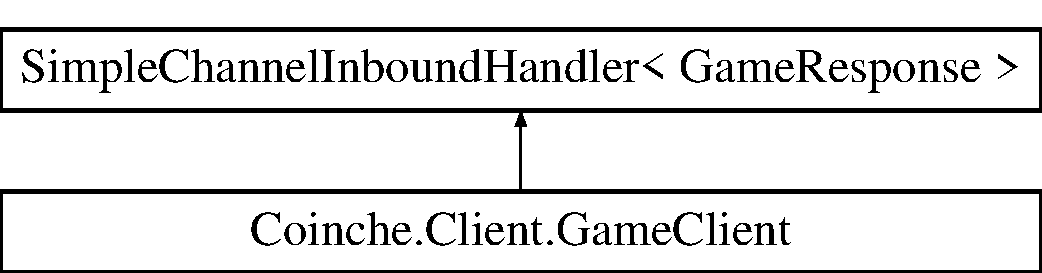
\includegraphics[height=2.000000cm]{class_coinche_1_1_client_1_1_game_client}
\end{center}
\end{figure}
\subsection*{Public Member Functions}
\begin{DoxyCompactItemize}
\item 
override void \hyperlink{class_coinche_1_1_client_1_1_game_client_a5764c84f4c58919f3ff21c874455509b}{Exception\+Caught} (I\+Channel\+Handler\+Context context, Exception exception)
\begin{DoxyCompactList}\small\item\em Print the caught exception \end{DoxyCompactList}\end{DoxyCompactItemize}
\subsection*{Protected Member Functions}
\begin{DoxyCompactItemize}
\item 
override void \hyperlink{class_coinche_1_1_client_1_1_game_client_a706d011a63f1277147e75475ff6a7d25}{Channel\+Read0} (I\+Channel\+Handler\+Context context, \hyperlink{class_coinche_1_1_google_1_1_protobuf_1_1_game_response}{Game\+Response} msg)
\begin{DoxyCompactList}\small\item\em Display the received response from the server \end{DoxyCompactList}\end{DoxyCompactItemize}


\subsection{Detailed Description}
Game client. 



\subsection{Member Function Documentation}
\mbox{\Hypertarget{class_coinche_1_1_client_1_1_game_client_a706d011a63f1277147e75475ff6a7d25}\label{class_coinche_1_1_client_1_1_game_client_a706d011a63f1277147e75475ff6a7d25}} 
\index{Coinche\+::\+Client\+::\+Game\+Client@{Coinche\+::\+Client\+::\+Game\+Client}!Channel\+Read0@{Channel\+Read0}}
\index{Channel\+Read0@{Channel\+Read0}!Coinche\+::\+Client\+::\+Game\+Client@{Coinche\+::\+Client\+::\+Game\+Client}}
\subsubsection{\texorpdfstring{Channel\+Read0()}{ChannelRead0()}}
{\footnotesize\ttfamily override void Coinche.\+Client.\+Game\+Client.\+Channel\+Read0 (\begin{DoxyParamCaption}\item[{I\+Channel\+Handler\+Context}]{context,  }\item[{\hyperlink{class_coinche_1_1_google_1_1_protobuf_1_1_game_response}{Game\+Response}}]{msg }\end{DoxyParamCaption})\hspace{0.3cm}{\ttfamily [inline]}, {\ttfamily [protected]}}



Display the received response from the server 


\begin{DoxyParams}{Parameters}
{\em context} & Context.\\
\hline
{\em msg} & Message.\\
\hline
\end{DoxyParams}
\mbox{\Hypertarget{class_coinche_1_1_client_1_1_game_client_a5764c84f4c58919f3ff21c874455509b}\label{class_coinche_1_1_client_1_1_game_client_a5764c84f4c58919f3ff21c874455509b}} 
\index{Coinche\+::\+Client\+::\+Game\+Client@{Coinche\+::\+Client\+::\+Game\+Client}!Exception\+Caught@{Exception\+Caught}}
\index{Exception\+Caught@{Exception\+Caught}!Coinche\+::\+Client\+::\+Game\+Client@{Coinche\+::\+Client\+::\+Game\+Client}}
\subsubsection{\texorpdfstring{Exception\+Caught()}{ExceptionCaught()}}
{\footnotesize\ttfamily override void Coinche.\+Client.\+Game\+Client.\+Exception\+Caught (\begin{DoxyParamCaption}\item[{I\+Channel\+Handler\+Context}]{context,  }\item[{Exception}]{exception }\end{DoxyParamCaption})\hspace{0.3cm}{\ttfamily [inline]}}



Print the caught exception 


\begin{DoxyParams}{Parameters}
{\em context} & Context.\\
\hline
{\em exception} & Exception.\\
\hline
\end{DoxyParams}


The documentation for this class was generated from the following file\+:\begin{DoxyCompactItemize}
\item 
Client/\+Core/Game\+Client.\+cs\end{DoxyCompactItemize}

\hypertarget{class_coinche_1_1_tools_1_1_game_info}{}\section{Coinche.\+Tools.\+Game\+Info Class Reference}
\label{class_coinche_1_1_tools_1_1_game_info}\index{Coinche.\+Tools.\+Game\+Info@{Coinche.\+Tools.\+Game\+Info}}


Tes messages to send to the players and the infos to update the game  


\subsection*{Public Member Functions}
\begin{DoxyCompactItemize}
\item 
\hyperlink{class_coinche_1_1_tools_1_1_game_info_a3c766aced6b335c4888fd5fd06ca098f}{Game\+Info} ()
\begin{DoxyCompactList}\small\item\em initializes the infos \end{DoxyCompactList}\end{DoxyCompactItemize}
\subsection*{Properties}
\begin{DoxyCompactItemize}
\item 
int \hyperlink{class_coinche_1_1_tools_1_1_game_info_aa5889e94191b88dfacc058569858ec38}{Private\+Player}\hspace{0.3cm}{\ttfamily  \mbox{[}get, set\mbox{]}}
\begin{DoxyCompactList}\small\item\em Message to send to a single player \end{DoxyCompactList}\item 
\mbox{\Hypertarget{class_coinche_1_1_tools_1_1_game_info_a9cdbe2b9e1e98582fb4e7b843894e4a7}\label{class_coinche_1_1_tools_1_1_game_info_a9cdbe2b9e1e98582fb4e7b843894e4a7}} 
string {\bfseries Private\+Message}\hspace{0.3cm}{\ttfamily  \mbox{[}get, set\mbox{]}}
\item 
string \hyperlink{class_coinche_1_1_tools_1_1_game_info_a0b839fbdcb8a923a7c1061adfb1e8586}{Public\+Message}\hspace{0.3cm}{\ttfamily  \mbox{[}get, set\mbox{]}}
\begin{DoxyCompactList}\small\item\em Message to send to every players \end{DoxyCompactList}\item 
Boolean \hyperlink{class_coinche_1_1_tools_1_1_game_info_ac591b0c4f8c2c2f90e6336b394d776c1}{Go\+To\+Next\+Step}\hspace{0.3cm}{\ttfamily  \mbox{[}get, set\mbox{]}}
\begin{DoxyCompactList}\small\item\em If true go to next step \end{DoxyCompactList}\item 
Boolean \hyperlink{class_coinche_1_1_tools_1_1_game_info_a5023dd4061549f0f91f1d4dfa7a50374}{Restart\+Round}\hspace{0.3cm}{\ttfamily  \mbox{[}get, set\mbox{]}}
\begin{DoxyCompactList}\small\item\em If true restart the round \end{DoxyCompactList}\item 
Boolean \hyperlink{class_coinche_1_1_tools_1_1_game_info_ac8e1f40fa1b2d65a4e6468e904600967}{Restart\+Game}\hspace{0.3cm}{\ttfamily  \mbox{[}get, set\mbox{]}}
\begin{DoxyCompactList}\small\item\em If true restart the game \end{DoxyCompactList}\item 
Boolean \hyperlink{class_coinche_1_1_tools_1_1_game_info_ad8e4babf051a6eb82792190097b50582}{Valid\+Turn}\hspace{0.3cm}{\ttfamily  \mbox{[}get, set\mbox{]}}
\begin{DoxyCompactList}\small\item\em If true we display the informations for the next player \end{DoxyCompactList}\item 
int \hyperlink{class_coinche_1_1_tools_1_1_game_info_ae516bdeec5b6602e12319890bbf4ee0c}{team\+Contract}\hspace{0.3cm}{\ttfamily  \mbox{[}get, set\mbox{]}}
\begin{DoxyCompactList}\small\item\em the number of the team who got the contract \end{DoxyCompactList}\item 
int \hyperlink{class_coinche_1_1_tools_1_1_game_info_acac3b4e483a564843e32ca5f7313cfb7}{points\+Bet}\hspace{0.3cm}{\ttfamily  \mbox{[}get, set\mbox{]}}
\begin{DoxyCompactList}\small\item\em the amount of points to make to win the contract \end{DoxyCompactList}\item 
Card\+Color \hyperlink{class_coinche_1_1_tools_1_1_game_info_ad547c22e23833dbd7833726d3a03da60}{color\+Bet}\hspace{0.3cm}{\ttfamily  \mbox{[}get, set\mbox{]}}
\begin{DoxyCompactList}\small\item\em the asset color for the round \end{DoxyCompactList}\item 
Boolean \hyperlink{class_coinche_1_1_tools_1_1_game_info_ab9f5ff2748e7a1059254408b8c591886}{all\+Assets}\hspace{0.3cm}{\ttfamily  \mbox{[}get, set\mbox{]}}
\begin{DoxyCompactList}\small\item\em true if the team wants to play with all assets \end{DoxyCompactList}\item 
Boolean \hyperlink{class_coinche_1_1_tools_1_1_game_info_a23fc3472540fb1bd3e8f93d441b4d11b}{none\+Assets}\hspace{0.3cm}{\ttfamily  \mbox{[}get, set\mbox{]}}
\begin{DoxyCompactList}\small\item\em true if the team wants to play with none assets \end{DoxyCompactList}\item 
int \hyperlink{class_coinche_1_1_tools_1_1_game_info_aa9b6fbfb2ff2fa1eca132a8309f49035}{new\+First\+Player}\hspace{0.3cm}{\ttfamily  \mbox{[}get, set\mbox{]}}
\begin{DoxyCompactList}\small\item\em the first player of the next step \end{DoxyCompactList}\item 
int \hyperlink{class_coinche_1_1_tools_1_1_game_info_aed3eb9ce4d7328b7db337cc90b48d672}{add\+Round\+Points\+Team1}\hspace{0.3cm}{\ttfamily  \mbox{[}get, set\mbox{]}}
\begin{DoxyCompactList}\small\item\em amount of points to add to team1 for this round \end{DoxyCompactList}\item 
int \hyperlink{class_coinche_1_1_tools_1_1_game_info_a80a720cfab6611699cd8b7160bb02e7b}{add\+Round\+Points\+Team2}\hspace{0.3cm}{\ttfamily  \mbox{[}get, set\mbox{]}}
\begin{DoxyCompactList}\small\item\em amount of points to add to team2 for this round \end{DoxyCompactList}\item 
int \hyperlink{class_coinche_1_1_tools_1_1_game_info_a847381ba8a7e85cd6201ad6d1e3eea12}{mult}\hspace{0.3cm}{\ttfamily  \mbox{[}get, set\mbox{]}}
\begin{DoxyCompactList}\small\item\em score multiplier (either 1, 2 or 4) \end{DoxyCompactList}\item 
Boolean \hyperlink{class_coinche_1_1_tools_1_1_game_info_aa340d1c2fea40ca6867671a67f8574f8}{passed\+Counter}\hspace{0.3cm}{\ttfamily  \mbox{[}get, set\mbox{]}}
\begin{DoxyCompactList}\small\item\em true if the first player of a team passed \end{DoxyCompactList}\item 
Boolean \hyperlink{class_coinche_1_1_tools_1_1_game_info_a07ac8659592be6506ea001886ef527d9}{belotte}\hspace{0.3cm}{\ttfamily  \mbox{[}get, set\mbox{]}}
\begin{DoxyCompactList}\small\item\em true if a player played a belotte \end{DoxyCompactList}\item 
int \hyperlink{class_coinche_1_1_tools_1_1_game_info_a43774aa31b83dd09b096074590c2448f}{team\+Belotte}\hspace{0.3cm}{\ttfamily  \mbox{[}get, set\mbox{]}}
\begin{DoxyCompactList}\small\item\em number of the team who played the belotte \end{DoxyCompactList}\end{DoxyCompactItemize}


\subsection{Detailed Description}
Tes messages to send to the players and the infos to update the game 



\subsection{Constructor \& Destructor Documentation}
\mbox{\Hypertarget{class_coinche_1_1_tools_1_1_game_info_a3c766aced6b335c4888fd5fd06ca098f}\label{class_coinche_1_1_tools_1_1_game_info_a3c766aced6b335c4888fd5fd06ca098f}} 
\index{Coinche\+::\+Tools\+::\+Game\+Info@{Coinche\+::\+Tools\+::\+Game\+Info}!Game\+Info@{Game\+Info}}
\index{Game\+Info@{Game\+Info}!Coinche\+::\+Tools\+::\+Game\+Info@{Coinche\+::\+Tools\+::\+Game\+Info}}
\subsubsection{\texorpdfstring{Game\+Info()}{GameInfo()}}
{\footnotesize\ttfamily Coinche.\+Tools.\+Game\+Info.\+Game\+Info (\begin{DoxyParamCaption}{ }\end{DoxyParamCaption})\hspace{0.3cm}{\ttfamily [inline]}}



initializes the infos 



\subsection{Property Documentation}
\mbox{\Hypertarget{class_coinche_1_1_tools_1_1_game_info_aed3eb9ce4d7328b7db337cc90b48d672}\label{class_coinche_1_1_tools_1_1_game_info_aed3eb9ce4d7328b7db337cc90b48d672}} 
\index{Coinche\+::\+Tools\+::\+Game\+Info@{Coinche\+::\+Tools\+::\+Game\+Info}!add\+Round\+Points\+Team1@{add\+Round\+Points\+Team1}}
\index{add\+Round\+Points\+Team1@{add\+Round\+Points\+Team1}!Coinche\+::\+Tools\+::\+Game\+Info@{Coinche\+::\+Tools\+::\+Game\+Info}}
\subsubsection{\texorpdfstring{add\+Round\+Points\+Team1}{addRoundPointsTeam1}}
{\footnotesize\ttfamily int Coinche.\+Tools.\+Game\+Info.\+add\+Round\+Points\+Team1\hspace{0.3cm}{\ttfamily [get]}, {\ttfamily [set]}}



amount of points to add to team1 for this round 

\mbox{\Hypertarget{class_coinche_1_1_tools_1_1_game_info_a80a720cfab6611699cd8b7160bb02e7b}\label{class_coinche_1_1_tools_1_1_game_info_a80a720cfab6611699cd8b7160bb02e7b}} 
\index{Coinche\+::\+Tools\+::\+Game\+Info@{Coinche\+::\+Tools\+::\+Game\+Info}!add\+Round\+Points\+Team2@{add\+Round\+Points\+Team2}}
\index{add\+Round\+Points\+Team2@{add\+Round\+Points\+Team2}!Coinche\+::\+Tools\+::\+Game\+Info@{Coinche\+::\+Tools\+::\+Game\+Info}}
\subsubsection{\texorpdfstring{add\+Round\+Points\+Team2}{addRoundPointsTeam2}}
{\footnotesize\ttfamily int Coinche.\+Tools.\+Game\+Info.\+add\+Round\+Points\+Team2\hspace{0.3cm}{\ttfamily [get]}, {\ttfamily [set]}}



amount of points to add to team2 for this round 

\mbox{\Hypertarget{class_coinche_1_1_tools_1_1_game_info_ab9f5ff2748e7a1059254408b8c591886}\label{class_coinche_1_1_tools_1_1_game_info_ab9f5ff2748e7a1059254408b8c591886}} 
\index{Coinche\+::\+Tools\+::\+Game\+Info@{Coinche\+::\+Tools\+::\+Game\+Info}!all\+Assets@{all\+Assets}}
\index{all\+Assets@{all\+Assets}!Coinche\+::\+Tools\+::\+Game\+Info@{Coinche\+::\+Tools\+::\+Game\+Info}}
\subsubsection{\texorpdfstring{all\+Assets}{allAssets}}
{\footnotesize\ttfamily Boolean Coinche.\+Tools.\+Game\+Info.\+all\+Assets\hspace{0.3cm}{\ttfamily [get]}, {\ttfamily [set]}}



true if the team wants to play with all assets 

\mbox{\Hypertarget{class_coinche_1_1_tools_1_1_game_info_a07ac8659592be6506ea001886ef527d9}\label{class_coinche_1_1_tools_1_1_game_info_a07ac8659592be6506ea001886ef527d9}} 
\index{Coinche\+::\+Tools\+::\+Game\+Info@{Coinche\+::\+Tools\+::\+Game\+Info}!belotte@{belotte}}
\index{belotte@{belotte}!Coinche\+::\+Tools\+::\+Game\+Info@{Coinche\+::\+Tools\+::\+Game\+Info}}
\subsubsection{\texorpdfstring{belotte}{belotte}}
{\footnotesize\ttfamily Boolean Coinche.\+Tools.\+Game\+Info.\+belotte\hspace{0.3cm}{\ttfamily [get]}, {\ttfamily [set]}}



true if a player played a belotte 

\mbox{\Hypertarget{class_coinche_1_1_tools_1_1_game_info_ad547c22e23833dbd7833726d3a03da60}\label{class_coinche_1_1_tools_1_1_game_info_ad547c22e23833dbd7833726d3a03da60}} 
\index{Coinche\+::\+Tools\+::\+Game\+Info@{Coinche\+::\+Tools\+::\+Game\+Info}!color\+Bet@{color\+Bet}}
\index{color\+Bet@{color\+Bet}!Coinche\+::\+Tools\+::\+Game\+Info@{Coinche\+::\+Tools\+::\+Game\+Info}}
\subsubsection{\texorpdfstring{color\+Bet}{colorBet}}
{\footnotesize\ttfamily Card\+Color Coinche.\+Tools.\+Game\+Info.\+color\+Bet\hspace{0.3cm}{\ttfamily [get]}, {\ttfamily [set]}}



the asset color for the round 

\mbox{\Hypertarget{class_coinche_1_1_tools_1_1_game_info_ac591b0c4f8c2c2f90e6336b394d776c1}\label{class_coinche_1_1_tools_1_1_game_info_ac591b0c4f8c2c2f90e6336b394d776c1}} 
\index{Coinche\+::\+Tools\+::\+Game\+Info@{Coinche\+::\+Tools\+::\+Game\+Info}!Go\+To\+Next\+Step@{Go\+To\+Next\+Step}}
\index{Go\+To\+Next\+Step@{Go\+To\+Next\+Step}!Coinche\+::\+Tools\+::\+Game\+Info@{Coinche\+::\+Tools\+::\+Game\+Info}}
\subsubsection{\texorpdfstring{Go\+To\+Next\+Step}{GoToNextStep}}
{\footnotesize\ttfamily Boolean Coinche.\+Tools.\+Game\+Info.\+Go\+To\+Next\+Step\hspace{0.3cm}{\ttfamily [get]}, {\ttfamily [set]}}



If true go to next step 

\mbox{\Hypertarget{class_coinche_1_1_tools_1_1_game_info_a847381ba8a7e85cd6201ad6d1e3eea12}\label{class_coinche_1_1_tools_1_1_game_info_a847381ba8a7e85cd6201ad6d1e3eea12}} 
\index{Coinche\+::\+Tools\+::\+Game\+Info@{Coinche\+::\+Tools\+::\+Game\+Info}!mult@{mult}}
\index{mult@{mult}!Coinche\+::\+Tools\+::\+Game\+Info@{Coinche\+::\+Tools\+::\+Game\+Info}}
\subsubsection{\texorpdfstring{mult}{mult}}
{\footnotesize\ttfamily int Coinche.\+Tools.\+Game\+Info.\+mult\hspace{0.3cm}{\ttfamily [get]}, {\ttfamily [set]}}



score multiplier (either 1, 2 or 4) 

\mbox{\Hypertarget{class_coinche_1_1_tools_1_1_game_info_aa9b6fbfb2ff2fa1eca132a8309f49035}\label{class_coinche_1_1_tools_1_1_game_info_aa9b6fbfb2ff2fa1eca132a8309f49035}} 
\index{Coinche\+::\+Tools\+::\+Game\+Info@{Coinche\+::\+Tools\+::\+Game\+Info}!new\+First\+Player@{new\+First\+Player}}
\index{new\+First\+Player@{new\+First\+Player}!Coinche\+::\+Tools\+::\+Game\+Info@{Coinche\+::\+Tools\+::\+Game\+Info}}
\subsubsection{\texorpdfstring{new\+First\+Player}{newFirstPlayer}}
{\footnotesize\ttfamily int Coinche.\+Tools.\+Game\+Info.\+new\+First\+Player\hspace{0.3cm}{\ttfamily [get]}, {\ttfamily [set]}}



the first player of the next step 

\mbox{\Hypertarget{class_coinche_1_1_tools_1_1_game_info_a23fc3472540fb1bd3e8f93d441b4d11b}\label{class_coinche_1_1_tools_1_1_game_info_a23fc3472540fb1bd3e8f93d441b4d11b}} 
\index{Coinche\+::\+Tools\+::\+Game\+Info@{Coinche\+::\+Tools\+::\+Game\+Info}!none\+Assets@{none\+Assets}}
\index{none\+Assets@{none\+Assets}!Coinche\+::\+Tools\+::\+Game\+Info@{Coinche\+::\+Tools\+::\+Game\+Info}}
\subsubsection{\texorpdfstring{none\+Assets}{noneAssets}}
{\footnotesize\ttfamily Boolean Coinche.\+Tools.\+Game\+Info.\+none\+Assets\hspace{0.3cm}{\ttfamily [get]}, {\ttfamily [set]}}



true if the team wants to play with none assets 

\mbox{\Hypertarget{class_coinche_1_1_tools_1_1_game_info_aa340d1c2fea40ca6867671a67f8574f8}\label{class_coinche_1_1_tools_1_1_game_info_aa340d1c2fea40ca6867671a67f8574f8}} 
\index{Coinche\+::\+Tools\+::\+Game\+Info@{Coinche\+::\+Tools\+::\+Game\+Info}!passed\+Counter@{passed\+Counter}}
\index{passed\+Counter@{passed\+Counter}!Coinche\+::\+Tools\+::\+Game\+Info@{Coinche\+::\+Tools\+::\+Game\+Info}}
\subsubsection{\texorpdfstring{passed\+Counter}{passedCounter}}
{\footnotesize\ttfamily Boolean Coinche.\+Tools.\+Game\+Info.\+passed\+Counter\hspace{0.3cm}{\ttfamily [get]}, {\ttfamily [set]}}



true if the first player of a team passed 

\mbox{\Hypertarget{class_coinche_1_1_tools_1_1_game_info_acac3b4e483a564843e32ca5f7313cfb7}\label{class_coinche_1_1_tools_1_1_game_info_acac3b4e483a564843e32ca5f7313cfb7}} 
\index{Coinche\+::\+Tools\+::\+Game\+Info@{Coinche\+::\+Tools\+::\+Game\+Info}!points\+Bet@{points\+Bet}}
\index{points\+Bet@{points\+Bet}!Coinche\+::\+Tools\+::\+Game\+Info@{Coinche\+::\+Tools\+::\+Game\+Info}}
\subsubsection{\texorpdfstring{points\+Bet}{pointsBet}}
{\footnotesize\ttfamily int Coinche.\+Tools.\+Game\+Info.\+points\+Bet\hspace{0.3cm}{\ttfamily [get]}, {\ttfamily [set]}}



the amount of points to make to win the contract 

\mbox{\Hypertarget{class_coinche_1_1_tools_1_1_game_info_aa5889e94191b88dfacc058569858ec38}\label{class_coinche_1_1_tools_1_1_game_info_aa5889e94191b88dfacc058569858ec38}} 
\index{Coinche\+::\+Tools\+::\+Game\+Info@{Coinche\+::\+Tools\+::\+Game\+Info}!Private\+Player@{Private\+Player}}
\index{Private\+Player@{Private\+Player}!Coinche\+::\+Tools\+::\+Game\+Info@{Coinche\+::\+Tools\+::\+Game\+Info}}
\subsubsection{\texorpdfstring{Private\+Player}{PrivatePlayer}}
{\footnotesize\ttfamily int Coinche.\+Tools.\+Game\+Info.\+Private\+Player\hspace{0.3cm}{\ttfamily [get]}, {\ttfamily [set]}}



Message to send to a single player 

\mbox{\Hypertarget{class_coinche_1_1_tools_1_1_game_info_a0b839fbdcb8a923a7c1061adfb1e8586}\label{class_coinche_1_1_tools_1_1_game_info_a0b839fbdcb8a923a7c1061adfb1e8586}} 
\index{Coinche\+::\+Tools\+::\+Game\+Info@{Coinche\+::\+Tools\+::\+Game\+Info}!Public\+Message@{Public\+Message}}
\index{Public\+Message@{Public\+Message}!Coinche\+::\+Tools\+::\+Game\+Info@{Coinche\+::\+Tools\+::\+Game\+Info}}
\subsubsection{\texorpdfstring{Public\+Message}{PublicMessage}}
{\footnotesize\ttfamily string Coinche.\+Tools.\+Game\+Info.\+Public\+Message\hspace{0.3cm}{\ttfamily [get]}, {\ttfamily [set]}}



Message to send to every players 

\mbox{\Hypertarget{class_coinche_1_1_tools_1_1_game_info_ac8e1f40fa1b2d65a4e6468e904600967}\label{class_coinche_1_1_tools_1_1_game_info_ac8e1f40fa1b2d65a4e6468e904600967}} 
\index{Coinche\+::\+Tools\+::\+Game\+Info@{Coinche\+::\+Tools\+::\+Game\+Info}!Restart\+Game@{Restart\+Game}}
\index{Restart\+Game@{Restart\+Game}!Coinche\+::\+Tools\+::\+Game\+Info@{Coinche\+::\+Tools\+::\+Game\+Info}}
\subsubsection{\texorpdfstring{Restart\+Game}{RestartGame}}
{\footnotesize\ttfamily Boolean Coinche.\+Tools.\+Game\+Info.\+Restart\+Game\hspace{0.3cm}{\ttfamily [get]}, {\ttfamily [set]}}



If true restart the game 

\mbox{\Hypertarget{class_coinche_1_1_tools_1_1_game_info_a5023dd4061549f0f91f1d4dfa7a50374}\label{class_coinche_1_1_tools_1_1_game_info_a5023dd4061549f0f91f1d4dfa7a50374}} 
\index{Coinche\+::\+Tools\+::\+Game\+Info@{Coinche\+::\+Tools\+::\+Game\+Info}!Restart\+Round@{Restart\+Round}}
\index{Restart\+Round@{Restart\+Round}!Coinche\+::\+Tools\+::\+Game\+Info@{Coinche\+::\+Tools\+::\+Game\+Info}}
\subsubsection{\texorpdfstring{Restart\+Round}{RestartRound}}
{\footnotesize\ttfamily Boolean Coinche.\+Tools.\+Game\+Info.\+Restart\+Round\hspace{0.3cm}{\ttfamily [get]}, {\ttfamily [set]}}



If true restart the round 

\mbox{\Hypertarget{class_coinche_1_1_tools_1_1_game_info_a43774aa31b83dd09b096074590c2448f}\label{class_coinche_1_1_tools_1_1_game_info_a43774aa31b83dd09b096074590c2448f}} 
\index{Coinche\+::\+Tools\+::\+Game\+Info@{Coinche\+::\+Tools\+::\+Game\+Info}!team\+Belotte@{team\+Belotte}}
\index{team\+Belotte@{team\+Belotte}!Coinche\+::\+Tools\+::\+Game\+Info@{Coinche\+::\+Tools\+::\+Game\+Info}}
\subsubsection{\texorpdfstring{team\+Belotte}{teamBelotte}}
{\footnotesize\ttfamily int Coinche.\+Tools.\+Game\+Info.\+team\+Belotte\hspace{0.3cm}{\ttfamily [get]}, {\ttfamily [set]}}



number of the team who played the belotte 

\mbox{\Hypertarget{class_coinche_1_1_tools_1_1_game_info_ae516bdeec5b6602e12319890bbf4ee0c}\label{class_coinche_1_1_tools_1_1_game_info_ae516bdeec5b6602e12319890bbf4ee0c}} 
\index{Coinche\+::\+Tools\+::\+Game\+Info@{Coinche\+::\+Tools\+::\+Game\+Info}!team\+Contract@{team\+Contract}}
\index{team\+Contract@{team\+Contract}!Coinche\+::\+Tools\+::\+Game\+Info@{Coinche\+::\+Tools\+::\+Game\+Info}}
\subsubsection{\texorpdfstring{team\+Contract}{teamContract}}
{\footnotesize\ttfamily int Coinche.\+Tools.\+Game\+Info.\+team\+Contract\hspace{0.3cm}{\ttfamily [get]}, {\ttfamily [set]}}



the number of the team who got the contract 

\mbox{\Hypertarget{class_coinche_1_1_tools_1_1_game_info_ad8e4babf051a6eb82792190097b50582}\label{class_coinche_1_1_tools_1_1_game_info_ad8e4babf051a6eb82792190097b50582}} 
\index{Coinche\+::\+Tools\+::\+Game\+Info@{Coinche\+::\+Tools\+::\+Game\+Info}!Valid\+Turn@{Valid\+Turn}}
\index{Valid\+Turn@{Valid\+Turn}!Coinche\+::\+Tools\+::\+Game\+Info@{Coinche\+::\+Tools\+::\+Game\+Info}}
\subsubsection{\texorpdfstring{Valid\+Turn}{ValidTurn}}
{\footnotesize\ttfamily Boolean Coinche.\+Tools.\+Game\+Info.\+Valid\+Turn\hspace{0.3cm}{\ttfamily [get]}, {\ttfamily [set]}}



If true we display the informations for the next player 



The documentation for this class was generated from the following file\+:\begin{DoxyCompactItemize}
\item 
Server/\+Tools/Game\+Info.\+cs\end{DoxyCompactItemize}

\hypertarget{class_coinche_1_1_server_1_1_game_manager}{}\section{Coinche.\+Server.\+Game\+Manager Class Reference}
\label{class_coinche_1_1_server_1_1_game_manager}\index{Coinche.\+Server.\+Game\+Manager@{Coinche.\+Server.\+Game\+Manager}}


Class to handle new connections comming from different clients  


Inheritance diagram for Coinche.\+Server.\+Game\+Manager\+:\begin{figure}[H]
\begin{center}
\leavevmode
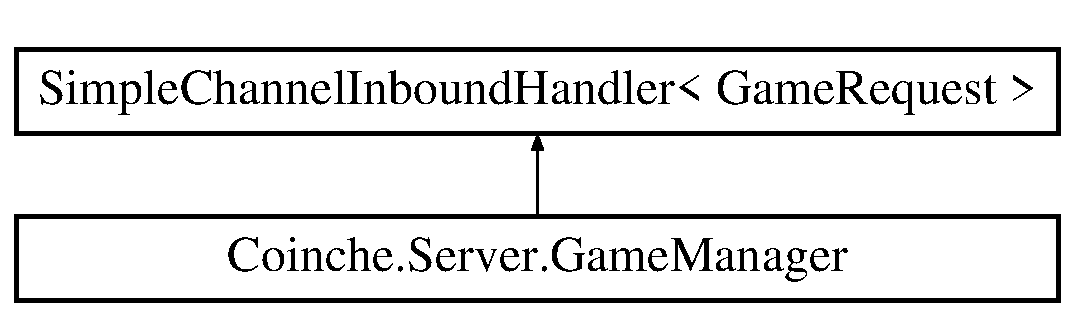
\includegraphics[height=2.000000cm]{class_coinche_1_1_server_1_1_game_manager}
\end{center}
\end{figure}
\subsection*{Public Member Functions}
\begin{DoxyCompactItemize}
\item 
\hyperlink{class_coinche_1_1_server_1_1_game_manager_ab9e920517c1b0486d86b0c3cdb8f2896}{Game\+Manager} ()
\begin{DoxyCompactList}\small\item\em Initializes a new instance of the T\+:\+Jcoinche.\+Server class. \end{DoxyCompactList}\item 
override void \hyperlink{class_coinche_1_1_server_1_1_game_manager_aaaa4563037a196f74811f9f35892c613}{Channel\+Active} (I\+Channel\+Handler\+Context context)
\begin{DoxyCompactList}\small\item\em First method when a player connects to the server Direct him to the first gameroom available \end{DoxyCompactList}\item 
override void \hyperlink{class_coinche_1_1_server_1_1_game_manager_a69ffe1493216ea1cdbaa0cbd2694df95}{Channel\+Inactive} (I\+Channel\+Handler\+Context context)
\begin{DoxyCompactList}\small\item\em Disconnects someone from our server \end{DoxyCompactList}\item 
override void \hyperlink{class_coinche_1_1_server_1_1_game_manager_a6f0b2a2abd6f793b8d45dcd8f41819a0}{Channel\+Read\+Complete} (I\+Channel\+Handler\+Context context)
\begin{DoxyCompactList}\small\item\em Flush the socket \end{DoxyCompactList}\item 
override void \hyperlink{class_coinche_1_1_server_1_1_game_manager_a87a33c57dcce28d543de561f7ab4134b}{Exception\+Caught} (I\+Channel\+Handler\+Context context, Exception exception)
\begin{DoxyCompactList}\small\item\em Get the exception and log it \end{DoxyCompactList}\end{DoxyCompactItemize}
\subsection*{Public Attributes}
\begin{DoxyCompactItemize}
\item 
override bool \hyperlink{class_coinche_1_1_server_1_1_game_manager_ac42b7e22b664b020a2c0daecdbf4ace3}{Is\+Sharable} =$>$ true
\begin{DoxyCompactList}\small\item\em Gets a value indicating whether this T\+:\+Jcoinche.\+Server.\+Game\+Server is sharable. \end{DoxyCompactList}\end{DoxyCompactItemize}
\subsection*{Protected Member Functions}
\begin{DoxyCompactItemize}
\item 
override void \hyperlink{class_coinche_1_1_server_1_1_game_manager_a94fb29dfd64df404419f8136c1d0c907}{Channel\+Read0} (I\+Channel\+Handler\+Context context, \hyperlink{class_coinche_1_1_google_1_1_protobuf_1_1_game_request}{Game\+Request} message)
\begin{DoxyCompactList}\small\item\em Read incomming message and send it to the corresponding \hyperlink{class_coinche_1_1_server_1_1_game_room}{Game\+Room} \end{DoxyCompactList}\end{DoxyCompactItemize}
\subsection*{Static Private Attributes}
\begin{DoxyCompactItemize}
\item 
static volatile List$<$ \hyperlink{class_coinche_1_1_server_1_1_game_room}{Game\+Room} $>$ \hyperlink{class_coinche_1_1_server_1_1_game_manager_abf914b45ad131ab37252a63d3c23ac39}{Rooms} = new List$<$\hyperlink{class_coinche_1_1_server_1_1_game_room}{Game\+Room}$>$()
\begin{DoxyCompactList}\small\item\em \hyperlink{class_coinche_1_1_server_1_1_game_room}{Game\+Room} where 4 players are gathered \end{DoxyCompactList}\item 
static \hyperlink{class_coinche_1_1_tools_1_1_logger}{Logger} \hyperlink{class_coinche_1_1_server_1_1_game_manager_a59f6b50ef1be82252b05d12fcbf16258}{Logger} = new \hyperlink{class_coinche_1_1_tools_1_1_logger}{Logger}()
\begin{DoxyCompactList}\small\item\em Gets the logger. \end{DoxyCompactList}\end{DoxyCompactItemize}


\subsection{Detailed Description}
Class to handle new connections comming from different clients 

This is only the T\+C\+P\+Layer, the business logic is implemented through the \hyperlink{class_coinche_1_1_server_1_1_game_room}{Game\+Room} object which possesses the rules 

\subsection{Constructor \& Destructor Documentation}
\mbox{\Hypertarget{class_coinche_1_1_server_1_1_game_manager_ab9e920517c1b0486d86b0c3cdb8f2896}\label{class_coinche_1_1_server_1_1_game_manager_ab9e920517c1b0486d86b0c3cdb8f2896}} 
\index{Coinche\+::\+Server\+::\+Game\+Manager@{Coinche\+::\+Server\+::\+Game\+Manager}!Game\+Manager@{Game\+Manager}}
\index{Game\+Manager@{Game\+Manager}!Coinche\+::\+Server\+::\+Game\+Manager@{Coinche\+::\+Server\+::\+Game\+Manager}}
\subsubsection{\texorpdfstring{Game\+Manager()}{GameManager()}}
{\footnotesize\ttfamily Coinche.\+Server.\+Game\+Manager.\+Game\+Manager (\begin{DoxyParamCaption}{ }\end{DoxyParamCaption})\hspace{0.3cm}{\ttfamily [inline]}}



Initializes a new instance of the T\+:\+Jcoinche.\+Server class. 

\hyperlink{namespace_coinche_1_1_server}{Server} is launched and listening on addr\+:port 

\subsection{Member Function Documentation}
\mbox{\Hypertarget{class_coinche_1_1_server_1_1_game_manager_aaaa4563037a196f74811f9f35892c613}\label{class_coinche_1_1_server_1_1_game_manager_aaaa4563037a196f74811f9f35892c613}} 
\index{Coinche\+::\+Server\+::\+Game\+Manager@{Coinche\+::\+Server\+::\+Game\+Manager}!Channel\+Active@{Channel\+Active}}
\index{Channel\+Active@{Channel\+Active}!Coinche\+::\+Server\+::\+Game\+Manager@{Coinche\+::\+Server\+::\+Game\+Manager}}
\subsubsection{\texorpdfstring{Channel\+Active()}{ChannelActive()}}
{\footnotesize\ttfamily override void Coinche.\+Server.\+Game\+Manager.\+Channel\+Active (\begin{DoxyParamCaption}\item[{I\+Channel\+Handler\+Context}]{context }\end{DoxyParamCaption})\hspace{0.3cm}{\ttfamily [inline]}}



First method when a player connects to the server Direct him to the first gameroom available 


\begin{DoxyParams}{Parameters}
{\em context} & Context.\\
\hline
\end{DoxyParams}
\mbox{\Hypertarget{class_coinche_1_1_server_1_1_game_manager_a69ffe1493216ea1cdbaa0cbd2694df95}\label{class_coinche_1_1_server_1_1_game_manager_a69ffe1493216ea1cdbaa0cbd2694df95}} 
\index{Coinche\+::\+Server\+::\+Game\+Manager@{Coinche\+::\+Server\+::\+Game\+Manager}!Channel\+Inactive@{Channel\+Inactive}}
\index{Channel\+Inactive@{Channel\+Inactive}!Coinche\+::\+Server\+::\+Game\+Manager@{Coinche\+::\+Server\+::\+Game\+Manager}}
\subsubsection{\texorpdfstring{Channel\+Inactive()}{ChannelInactive()}}
{\footnotesize\ttfamily override void Coinche.\+Server.\+Game\+Manager.\+Channel\+Inactive (\begin{DoxyParamCaption}\item[{I\+Channel\+Handler\+Context}]{context }\end{DoxyParamCaption})\hspace{0.3cm}{\ttfamily [inline]}}



Disconnects someone from our server 


\begin{DoxyParams}{Parameters}
{\em context} & Context.\\
\hline
\end{DoxyParams}
\mbox{\Hypertarget{class_coinche_1_1_server_1_1_game_manager_a94fb29dfd64df404419f8136c1d0c907}\label{class_coinche_1_1_server_1_1_game_manager_a94fb29dfd64df404419f8136c1d0c907}} 
\index{Coinche\+::\+Server\+::\+Game\+Manager@{Coinche\+::\+Server\+::\+Game\+Manager}!Channel\+Read0@{Channel\+Read0}}
\index{Channel\+Read0@{Channel\+Read0}!Coinche\+::\+Server\+::\+Game\+Manager@{Coinche\+::\+Server\+::\+Game\+Manager}}
\subsubsection{\texorpdfstring{Channel\+Read0()}{ChannelRead0()}}
{\footnotesize\ttfamily override void Coinche.\+Server.\+Game\+Manager.\+Channel\+Read0 (\begin{DoxyParamCaption}\item[{I\+Channel\+Handler\+Context}]{context,  }\item[{\hyperlink{class_coinche_1_1_google_1_1_protobuf_1_1_game_request}{Game\+Request}}]{message }\end{DoxyParamCaption})\hspace{0.3cm}{\ttfamily [inline]}, {\ttfamily [protected]}}



Read incomming message and send it to the corresponding \hyperlink{class_coinche_1_1_server_1_1_game_room}{Game\+Room} 


\begin{DoxyParams}{Parameters}
{\em context} & Context.\\
\hline
{\em message} & Message.\\
\hline
\end{DoxyParams}
\mbox{\Hypertarget{class_coinche_1_1_server_1_1_game_manager_a6f0b2a2abd6f793b8d45dcd8f41819a0}\label{class_coinche_1_1_server_1_1_game_manager_a6f0b2a2abd6f793b8d45dcd8f41819a0}} 
\index{Coinche\+::\+Server\+::\+Game\+Manager@{Coinche\+::\+Server\+::\+Game\+Manager}!Channel\+Read\+Complete@{Channel\+Read\+Complete}}
\index{Channel\+Read\+Complete@{Channel\+Read\+Complete}!Coinche\+::\+Server\+::\+Game\+Manager@{Coinche\+::\+Server\+::\+Game\+Manager}}
\subsubsection{\texorpdfstring{Channel\+Read\+Complete()}{ChannelReadComplete()}}
{\footnotesize\ttfamily override void Coinche.\+Server.\+Game\+Manager.\+Channel\+Read\+Complete (\begin{DoxyParamCaption}\item[{I\+Channel\+Handler\+Context}]{context }\end{DoxyParamCaption})}



Flush the socket 


\begin{DoxyParams}{Parameters}
{\em context} & Context.\\
\hline
\end{DoxyParams}
\mbox{\Hypertarget{class_coinche_1_1_server_1_1_game_manager_a87a33c57dcce28d543de561f7ab4134b}\label{class_coinche_1_1_server_1_1_game_manager_a87a33c57dcce28d543de561f7ab4134b}} 
\index{Coinche\+::\+Server\+::\+Game\+Manager@{Coinche\+::\+Server\+::\+Game\+Manager}!Exception\+Caught@{Exception\+Caught}}
\index{Exception\+Caught@{Exception\+Caught}!Coinche\+::\+Server\+::\+Game\+Manager@{Coinche\+::\+Server\+::\+Game\+Manager}}
\subsubsection{\texorpdfstring{Exception\+Caught()}{ExceptionCaught()}}
{\footnotesize\ttfamily override void Coinche.\+Server.\+Game\+Manager.\+Exception\+Caught (\begin{DoxyParamCaption}\item[{I\+Channel\+Handler\+Context}]{context,  }\item[{Exception}]{exception }\end{DoxyParamCaption})\hspace{0.3cm}{\ttfamily [inline]}}



Get the exception and log it 


\begin{DoxyParams}{Parameters}
{\em context} & Context.\\
\hline
{\em exception} & Exception.\\
\hline
\end{DoxyParams}


\subsection{Member Data Documentation}
\mbox{\Hypertarget{class_coinche_1_1_server_1_1_game_manager_ac42b7e22b664b020a2c0daecdbf4ace3}\label{class_coinche_1_1_server_1_1_game_manager_ac42b7e22b664b020a2c0daecdbf4ace3}} 
\index{Coinche\+::\+Server\+::\+Game\+Manager@{Coinche\+::\+Server\+::\+Game\+Manager}!Is\+Sharable@{Is\+Sharable}}
\index{Is\+Sharable@{Is\+Sharable}!Coinche\+::\+Server\+::\+Game\+Manager@{Coinche\+::\+Server\+::\+Game\+Manager}}
\subsubsection{\texorpdfstring{Is\+Sharable}{IsSharable}}
{\footnotesize\ttfamily override bool Coinche.\+Server.\+Game\+Manager.\+Is\+Sharable =$>$ true}



Gets a value indicating whether this T\+:\+Jcoinche.\+Server.\+Game\+Server is sharable. 

{\ttfamily true} if is sharable; otherwise, {\ttfamily false}.\mbox{\Hypertarget{class_coinche_1_1_server_1_1_game_manager_a59f6b50ef1be82252b05d12fcbf16258}\label{class_coinche_1_1_server_1_1_game_manager_a59f6b50ef1be82252b05d12fcbf16258}} 
\index{Coinche\+::\+Server\+::\+Game\+Manager@{Coinche\+::\+Server\+::\+Game\+Manager}!Logger@{Logger}}
\index{Logger@{Logger}!Coinche\+::\+Server\+::\+Game\+Manager@{Coinche\+::\+Server\+::\+Game\+Manager}}
\subsubsection{\texorpdfstring{Logger}{Logger}}
{\footnotesize\ttfamily \hyperlink{class_coinche_1_1_tools_1_1_logger}{Logger} Coinche.\+Server.\+Game\+Manager.\+Logger = new \hyperlink{class_coinche_1_1_tools_1_1_logger}{Logger}()\hspace{0.3cm}{\ttfamily [static]}, {\ttfamily [private]}}



Gets the logger. 

The logger.\mbox{\Hypertarget{class_coinche_1_1_server_1_1_game_manager_abf914b45ad131ab37252a63d3c23ac39}\label{class_coinche_1_1_server_1_1_game_manager_abf914b45ad131ab37252a63d3c23ac39}} 
\index{Coinche\+::\+Server\+::\+Game\+Manager@{Coinche\+::\+Server\+::\+Game\+Manager}!Rooms@{Rooms}}
\index{Rooms@{Rooms}!Coinche\+::\+Server\+::\+Game\+Manager@{Coinche\+::\+Server\+::\+Game\+Manager}}
\subsubsection{\texorpdfstring{Rooms}{Rooms}}
{\footnotesize\ttfamily volatile List$<$\hyperlink{class_coinche_1_1_server_1_1_game_room}{Game\+Room}$>$ Coinche.\+Server.\+Game\+Manager.\+Rooms = new List$<$\hyperlink{class_coinche_1_1_server_1_1_game_room}{Game\+Room}$>$()\hspace{0.3cm}{\ttfamily [static]}, {\ttfamily [private]}}



\hyperlink{class_coinche_1_1_server_1_1_game_room}{Game\+Room} where 4 players are gathered 



The documentation for this class was generated from the following file\+:\begin{DoxyCompactItemize}
\item 
Server/\+Core/Game\+Manager.\+cs\end{DoxyCompactItemize}

\hypertarget{class_coinche_1_1_google_1_1_protobuf_1_1_game_request}{}\section{Coinche.\+Google.\+Protobuf.\+Game\+Request Class Reference}
\label{class_coinche_1_1_google_1_1_protobuf_1_1_game_request}\index{Coinche.\+Google.\+Protobuf.\+Game\+Request@{Coinche.\+Google.\+Protobuf.\+Game\+Request}}
Inheritance diagram for Coinche.\+Google.\+Protobuf.\+Game\+Request\+:\begin{figure}[H]
\begin{center}
\leavevmode
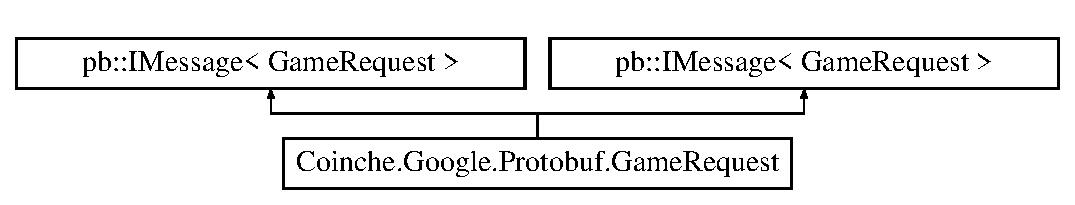
\includegraphics[height=2.000000cm]{class_coinche_1_1_google_1_1_protobuf_1_1_game_request}
\end{center}
\end{figure}
\subsection*{Public Member Functions}
\begin{DoxyCompactItemize}
\item 
\mbox{\Hypertarget{class_coinche_1_1_google_1_1_protobuf_1_1_game_request_a1d29f987b51c41d58a992550111c8d77}\label{class_coinche_1_1_google_1_1_protobuf_1_1_game_request_a1d29f987b51c41d58a992550111c8d77}} 
{\bfseries Game\+Request} (\hyperlink{class_coinche_1_1_google_1_1_protobuf_1_1_game_request}{Game\+Request} other)
\item 
\mbox{\Hypertarget{class_coinche_1_1_google_1_1_protobuf_1_1_game_request_afda8ec24e639da78db52800e98587d63}\label{class_coinche_1_1_google_1_1_protobuf_1_1_game_request_afda8ec24e639da78db52800e98587d63}} 
\hyperlink{class_coinche_1_1_google_1_1_protobuf_1_1_game_request}{Game\+Request} {\bfseries Clone} ()
\item 
\mbox{\Hypertarget{class_coinche_1_1_google_1_1_protobuf_1_1_game_request_a8912ff23d5acb3006a648aa292f24d82}\label{class_coinche_1_1_google_1_1_protobuf_1_1_game_request_a8912ff23d5acb3006a648aa292f24d82}} 
override bool {\bfseries Equals} (object other)
\item 
\mbox{\Hypertarget{class_coinche_1_1_google_1_1_protobuf_1_1_game_request_af439b94581949ebbc1807b4211d032b5}\label{class_coinche_1_1_google_1_1_protobuf_1_1_game_request_af439b94581949ebbc1807b4211d032b5}} 
bool {\bfseries Equals} (\hyperlink{class_coinche_1_1_google_1_1_protobuf_1_1_game_request}{Game\+Request} other)
\item 
\mbox{\Hypertarget{class_coinche_1_1_google_1_1_protobuf_1_1_game_request_ac376e84329a8f8f8821999b62a6db3d8}\label{class_coinche_1_1_google_1_1_protobuf_1_1_game_request_ac376e84329a8f8f8821999b62a6db3d8}} 
override int {\bfseries Get\+Hash\+Code} ()
\item 
\mbox{\Hypertarget{class_coinche_1_1_google_1_1_protobuf_1_1_game_request_a6b98ae0b06aa78d0369f65b81ca677b6}\label{class_coinche_1_1_google_1_1_protobuf_1_1_game_request_a6b98ae0b06aa78d0369f65b81ca677b6}} 
override string {\bfseries To\+String} ()
\item 
\mbox{\Hypertarget{class_coinche_1_1_google_1_1_protobuf_1_1_game_request_a0c2345787cdc5861832e873435efc270}\label{class_coinche_1_1_google_1_1_protobuf_1_1_game_request_a0c2345787cdc5861832e873435efc270}} 
void {\bfseries Write\+To} (pb\+::\+Coded\+Output\+Stream output)
\item 
\mbox{\Hypertarget{class_coinche_1_1_google_1_1_protobuf_1_1_game_request_a987e48747e64faec5e17851a6ea5ea3c}\label{class_coinche_1_1_google_1_1_protobuf_1_1_game_request_a987e48747e64faec5e17851a6ea5ea3c}} 
int {\bfseries Calculate\+Size} ()
\item 
\mbox{\Hypertarget{class_coinche_1_1_google_1_1_protobuf_1_1_game_request_aa124e890b22980c0ff98339a597393b9}\label{class_coinche_1_1_google_1_1_protobuf_1_1_game_request_aa124e890b22980c0ff98339a597393b9}} 
void {\bfseries Merge\+From} (\hyperlink{class_coinche_1_1_google_1_1_protobuf_1_1_game_request}{Game\+Request} other)
\item 
\mbox{\Hypertarget{class_coinche_1_1_google_1_1_protobuf_1_1_game_request_a52fe24d58b6d250d632ed6def954e5e7}\label{class_coinche_1_1_google_1_1_protobuf_1_1_game_request_a52fe24d58b6d250d632ed6def954e5e7}} 
void {\bfseries Merge\+From} (pb\+::\+Coded\+Input\+Stream input)
\item 
\mbox{\Hypertarget{class_coinche_1_1_google_1_1_protobuf_1_1_game_request_a1d29f987b51c41d58a992550111c8d77}\label{class_coinche_1_1_google_1_1_protobuf_1_1_game_request_a1d29f987b51c41d58a992550111c8d77}} 
{\bfseries Game\+Request} (\hyperlink{class_coinche_1_1_google_1_1_protobuf_1_1_game_request}{Game\+Request} other)
\item 
\mbox{\Hypertarget{class_coinche_1_1_google_1_1_protobuf_1_1_game_request_afda8ec24e639da78db52800e98587d63}\label{class_coinche_1_1_google_1_1_protobuf_1_1_game_request_afda8ec24e639da78db52800e98587d63}} 
\hyperlink{class_coinche_1_1_google_1_1_protobuf_1_1_game_request}{Game\+Request} {\bfseries Clone} ()
\item 
\mbox{\Hypertarget{class_coinche_1_1_google_1_1_protobuf_1_1_game_request_a8912ff23d5acb3006a648aa292f24d82}\label{class_coinche_1_1_google_1_1_protobuf_1_1_game_request_a8912ff23d5acb3006a648aa292f24d82}} 
override bool {\bfseries Equals} (object other)
\item 
\mbox{\Hypertarget{class_coinche_1_1_google_1_1_protobuf_1_1_game_request_af439b94581949ebbc1807b4211d032b5}\label{class_coinche_1_1_google_1_1_protobuf_1_1_game_request_af439b94581949ebbc1807b4211d032b5}} 
bool {\bfseries Equals} (\hyperlink{class_coinche_1_1_google_1_1_protobuf_1_1_game_request}{Game\+Request} other)
\item 
\mbox{\Hypertarget{class_coinche_1_1_google_1_1_protobuf_1_1_game_request_ac376e84329a8f8f8821999b62a6db3d8}\label{class_coinche_1_1_google_1_1_protobuf_1_1_game_request_ac376e84329a8f8f8821999b62a6db3d8}} 
override int {\bfseries Get\+Hash\+Code} ()
\item 
\mbox{\Hypertarget{class_coinche_1_1_google_1_1_protobuf_1_1_game_request_a6b98ae0b06aa78d0369f65b81ca677b6}\label{class_coinche_1_1_google_1_1_protobuf_1_1_game_request_a6b98ae0b06aa78d0369f65b81ca677b6}} 
override string {\bfseries To\+String} ()
\item 
\mbox{\Hypertarget{class_coinche_1_1_google_1_1_protobuf_1_1_game_request_a0c2345787cdc5861832e873435efc270}\label{class_coinche_1_1_google_1_1_protobuf_1_1_game_request_a0c2345787cdc5861832e873435efc270}} 
void {\bfseries Write\+To} (pb\+::\+Coded\+Output\+Stream output)
\item 
\mbox{\Hypertarget{class_coinche_1_1_google_1_1_protobuf_1_1_game_request_a987e48747e64faec5e17851a6ea5ea3c}\label{class_coinche_1_1_google_1_1_protobuf_1_1_game_request_a987e48747e64faec5e17851a6ea5ea3c}} 
int {\bfseries Calculate\+Size} ()
\item 
\mbox{\Hypertarget{class_coinche_1_1_google_1_1_protobuf_1_1_game_request_aa124e890b22980c0ff98339a597393b9}\label{class_coinche_1_1_google_1_1_protobuf_1_1_game_request_aa124e890b22980c0ff98339a597393b9}} 
void {\bfseries Merge\+From} (\hyperlink{class_coinche_1_1_google_1_1_protobuf_1_1_game_request}{Game\+Request} other)
\item 
\mbox{\Hypertarget{class_coinche_1_1_google_1_1_protobuf_1_1_game_request_a52fe24d58b6d250d632ed6def954e5e7}\label{class_coinche_1_1_google_1_1_protobuf_1_1_game_request_a52fe24d58b6d250d632ed6def954e5e7}} 
void {\bfseries Merge\+From} (pb\+::\+Coded\+Input\+Stream input)
\end{DoxyCompactItemize}
\subsection*{Public Attributes}
\begin{DoxyCompactItemize}
\item 
const int \hyperlink{class_coinche_1_1_google_1_1_protobuf_1_1_game_request_ab8aaf361fd25dc835cdcdf47aebb47b5}{Play\+Field\+Number} = 1
\begin{DoxyCompactList}\small\item\em Field number for the \char`\"{}play\char`\"{} field.\end{DoxyCompactList}\end{DoxyCompactItemize}
\subsection*{Properties}
\begin{DoxyCompactItemize}
\item 
\mbox{\Hypertarget{class_coinche_1_1_google_1_1_protobuf_1_1_game_request_ae323bbaf87bb01874f82e4e1bb0e3ba8}\label{class_coinche_1_1_google_1_1_protobuf_1_1_game_request_ae323bbaf87bb01874f82e4e1bb0e3ba8}} 
static pb\+::\+Message\+Parser$<$ \hyperlink{class_coinche_1_1_google_1_1_protobuf_1_1_game_request}{Game\+Request} $>$ {\bfseries Parser}\hspace{0.3cm}{\ttfamily  \mbox{[}get\mbox{]}}
\item 
\mbox{\Hypertarget{class_coinche_1_1_google_1_1_protobuf_1_1_game_request_a28eca4d785d844550fdcbf7c3a354ddf}\label{class_coinche_1_1_google_1_1_protobuf_1_1_game_request_a28eca4d785d844550fdcbf7c3a354ddf}} 
static pbr\+::\+Message\+Descriptor {\bfseries Descriptor}\hspace{0.3cm}{\ttfamily  \mbox{[}get\mbox{]}}
\item 
\mbox{\Hypertarget{class_coinche_1_1_google_1_1_protobuf_1_1_game_request_af3afd1c61a0fe717f5672ce3dd7adc0f}\label{class_coinche_1_1_google_1_1_protobuf_1_1_game_request_af3afd1c61a0fe717f5672ce3dd7adc0f}} 
pbr\+::\+Message\+Descriptor pb\+::\+I\+Message. {\bfseries Descriptor}\hspace{0.3cm}{\ttfamily  \mbox{[}get\mbox{]}}
\item 
\mbox{\Hypertarget{class_coinche_1_1_google_1_1_protobuf_1_1_game_request_a7c66f830a9141b27c66d76e732b51dec}\label{class_coinche_1_1_google_1_1_protobuf_1_1_game_request_a7c66f830a9141b27c66d76e732b51dec}} 
string {\bfseries Play}\hspace{0.3cm}{\ttfamily  \mbox{[}get, set\mbox{]}}
\end{DoxyCompactItemize}
\subsection*{Private Member Functions}
\begin{DoxyCompactItemize}
\item 
\mbox{\Hypertarget{class_coinche_1_1_google_1_1_protobuf_1_1_game_request_a171e29f804e27af68454bfeb3862b58e}\label{class_coinche_1_1_google_1_1_protobuf_1_1_game_request_a171e29f804e27af68454bfeb3862b58e}} 
partial void {\bfseries On\+Construction} ()
\item 
\mbox{\Hypertarget{class_coinche_1_1_google_1_1_protobuf_1_1_game_request_a171e29f804e27af68454bfeb3862b58e}\label{class_coinche_1_1_google_1_1_protobuf_1_1_game_request_a171e29f804e27af68454bfeb3862b58e}} 
partial void {\bfseries On\+Construction} ()
\end{DoxyCompactItemize}
\subsection*{Private Attributes}
\begin{DoxyCompactItemize}
\item 
\mbox{\Hypertarget{class_coinche_1_1_google_1_1_protobuf_1_1_game_request_aef5067764431d1a990969f8eb043d4a9}\label{class_coinche_1_1_google_1_1_protobuf_1_1_game_request_aef5067764431d1a990969f8eb043d4a9}} 
string {\bfseries play\+\_\+} = \char`\"{}\char`\"{}
\end{DoxyCompactItemize}
\subsection*{Static Private Attributes}
\begin{DoxyCompactItemize}
\item 
\mbox{\Hypertarget{class_coinche_1_1_google_1_1_protobuf_1_1_game_request_a0095926611e6c62b0b43db4faf0303cc}\label{class_coinche_1_1_google_1_1_protobuf_1_1_game_request_a0095926611e6c62b0b43db4faf0303cc}} 
static readonly pb\+::\+Message\+Parser$<$ \hyperlink{class_coinche_1_1_google_1_1_protobuf_1_1_game_request}{Game\+Request} $>$ {\bfseries \+\_\+parser} = new pb\+::\+Message\+Parser$<$\hyperlink{class_coinche_1_1_google_1_1_protobuf_1_1_game_request}{Game\+Request}$>$(() =$>$ new \hyperlink{class_coinche_1_1_google_1_1_protobuf_1_1_game_request}{Game\+Request}())
\end{DoxyCompactItemize}


\subsection{Member Data Documentation}
\mbox{\Hypertarget{class_coinche_1_1_google_1_1_protobuf_1_1_game_request_ab8aaf361fd25dc835cdcdf47aebb47b5}\label{class_coinche_1_1_google_1_1_protobuf_1_1_game_request_ab8aaf361fd25dc835cdcdf47aebb47b5}} 
\index{Coinche\+::\+Google\+::\+Protobuf\+::\+Game\+Request@{Coinche\+::\+Google\+::\+Protobuf\+::\+Game\+Request}!Play\+Field\+Number@{Play\+Field\+Number}}
\index{Play\+Field\+Number@{Play\+Field\+Number}!Coinche\+::\+Google\+::\+Protobuf\+::\+Game\+Request@{Coinche\+::\+Google\+::\+Protobuf\+::\+Game\+Request}}
\subsubsection{\texorpdfstring{Play\+Field\+Number}{PlayFieldNumber}}
{\footnotesize\ttfamily const int Coinche.\+Google.\+Protobuf.\+Game\+Request.\+Play\+Field\+Number = 1}



Field number for the \char`\"{}play\char`\"{} field.



The documentation for this class was generated from the following file\+:\begin{DoxyCompactItemize}
\item 
Client/\+Protobuf/Coinche\+Protocol.\+cs\end{DoxyCompactItemize}

\hypertarget{class_coinche_1_1_google_1_1_protobuf_1_1_game_response}{}\section{Coinche.\+Google.\+Protobuf.\+Game\+Response Class Reference}
\label{class_coinche_1_1_google_1_1_protobuf_1_1_game_response}\index{Coinche.\+Google.\+Protobuf.\+Game\+Response@{Coinche.\+Google.\+Protobuf.\+Game\+Response}}
Inheritance diagram for Coinche.\+Google.\+Protobuf.\+Game\+Response\+:\begin{figure}[H]
\begin{center}
\leavevmode
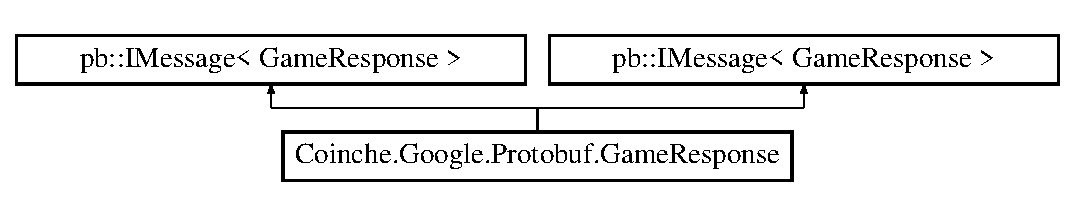
\includegraphics[height=2.000000cm]{class_coinche_1_1_google_1_1_protobuf_1_1_game_response}
\end{center}
\end{figure}
\subsection*{Public Member Functions}
\begin{DoxyCompactItemize}
\item 
\mbox{\Hypertarget{class_coinche_1_1_google_1_1_protobuf_1_1_game_response_ac0a4626c706d831cfcf734f0b4a09de9}\label{class_coinche_1_1_google_1_1_protobuf_1_1_game_response_ac0a4626c706d831cfcf734f0b4a09de9}} 
{\bfseries Game\+Response} (\hyperlink{class_coinche_1_1_google_1_1_protobuf_1_1_game_response}{Game\+Response} other)
\item 
\mbox{\Hypertarget{class_coinche_1_1_google_1_1_protobuf_1_1_game_response_a09023009f7dc34361db733f7aa5c425d}\label{class_coinche_1_1_google_1_1_protobuf_1_1_game_response_a09023009f7dc34361db733f7aa5c425d}} 
\hyperlink{class_coinche_1_1_google_1_1_protobuf_1_1_game_response}{Game\+Response} {\bfseries Clone} ()
\item 
\mbox{\Hypertarget{class_coinche_1_1_google_1_1_protobuf_1_1_game_response_a6e214c086e085093b948fde643c23582}\label{class_coinche_1_1_google_1_1_protobuf_1_1_game_response_a6e214c086e085093b948fde643c23582}} 
override bool {\bfseries Equals} (object other)
\item 
\mbox{\Hypertarget{class_coinche_1_1_google_1_1_protobuf_1_1_game_response_a7aa01a250f07fb90d710aa7a4ef9a19c}\label{class_coinche_1_1_google_1_1_protobuf_1_1_game_response_a7aa01a250f07fb90d710aa7a4ef9a19c}} 
bool {\bfseries Equals} (\hyperlink{class_coinche_1_1_google_1_1_protobuf_1_1_game_response}{Game\+Response} other)
\item 
\mbox{\Hypertarget{class_coinche_1_1_google_1_1_protobuf_1_1_game_response_ad5527f94a2253c52acf2cac1719ad6fc}\label{class_coinche_1_1_google_1_1_protobuf_1_1_game_response_ad5527f94a2253c52acf2cac1719ad6fc}} 
override int {\bfseries Get\+Hash\+Code} ()
\item 
\mbox{\Hypertarget{class_coinche_1_1_google_1_1_protobuf_1_1_game_response_a10d3b1dd26cb1c0ee084cddbcfc1de4a}\label{class_coinche_1_1_google_1_1_protobuf_1_1_game_response_a10d3b1dd26cb1c0ee084cddbcfc1de4a}} 
override string {\bfseries To\+String} ()
\item 
\mbox{\Hypertarget{class_coinche_1_1_google_1_1_protobuf_1_1_game_response_a7e2f8f7eeeb526f58dc1e3228cf2c04a}\label{class_coinche_1_1_google_1_1_protobuf_1_1_game_response_a7e2f8f7eeeb526f58dc1e3228cf2c04a}} 
void {\bfseries Write\+To} (pb\+::\+Coded\+Output\+Stream output)
\item 
\mbox{\Hypertarget{class_coinche_1_1_google_1_1_protobuf_1_1_game_response_a7966b0805c13b7883d4f18048aae509f}\label{class_coinche_1_1_google_1_1_protobuf_1_1_game_response_a7966b0805c13b7883d4f18048aae509f}} 
int {\bfseries Calculate\+Size} ()
\item 
\mbox{\Hypertarget{class_coinche_1_1_google_1_1_protobuf_1_1_game_response_a8180e18acfa95d164878f96a614c1d78}\label{class_coinche_1_1_google_1_1_protobuf_1_1_game_response_a8180e18acfa95d164878f96a614c1d78}} 
void {\bfseries Merge\+From} (\hyperlink{class_coinche_1_1_google_1_1_protobuf_1_1_game_response}{Game\+Response} other)
\item 
\mbox{\Hypertarget{class_coinche_1_1_google_1_1_protobuf_1_1_game_response_a39f44c99beef309bf97a049f870651e3}\label{class_coinche_1_1_google_1_1_protobuf_1_1_game_response_a39f44c99beef309bf97a049f870651e3}} 
void {\bfseries Merge\+From} (pb\+::\+Coded\+Input\+Stream input)
\item 
\mbox{\Hypertarget{class_coinche_1_1_google_1_1_protobuf_1_1_game_response_ac0a4626c706d831cfcf734f0b4a09de9}\label{class_coinche_1_1_google_1_1_protobuf_1_1_game_response_ac0a4626c706d831cfcf734f0b4a09de9}} 
{\bfseries Game\+Response} (\hyperlink{class_coinche_1_1_google_1_1_protobuf_1_1_game_response}{Game\+Response} other)
\item 
\mbox{\Hypertarget{class_coinche_1_1_google_1_1_protobuf_1_1_game_response_a09023009f7dc34361db733f7aa5c425d}\label{class_coinche_1_1_google_1_1_protobuf_1_1_game_response_a09023009f7dc34361db733f7aa5c425d}} 
\hyperlink{class_coinche_1_1_google_1_1_protobuf_1_1_game_response}{Game\+Response} {\bfseries Clone} ()
\item 
\mbox{\Hypertarget{class_coinche_1_1_google_1_1_protobuf_1_1_game_response_a6e214c086e085093b948fde643c23582}\label{class_coinche_1_1_google_1_1_protobuf_1_1_game_response_a6e214c086e085093b948fde643c23582}} 
override bool {\bfseries Equals} (object other)
\item 
\mbox{\Hypertarget{class_coinche_1_1_google_1_1_protobuf_1_1_game_response_a7aa01a250f07fb90d710aa7a4ef9a19c}\label{class_coinche_1_1_google_1_1_protobuf_1_1_game_response_a7aa01a250f07fb90d710aa7a4ef9a19c}} 
bool {\bfseries Equals} (\hyperlink{class_coinche_1_1_google_1_1_protobuf_1_1_game_response}{Game\+Response} other)
\item 
\mbox{\Hypertarget{class_coinche_1_1_google_1_1_protobuf_1_1_game_response_ad5527f94a2253c52acf2cac1719ad6fc}\label{class_coinche_1_1_google_1_1_protobuf_1_1_game_response_ad5527f94a2253c52acf2cac1719ad6fc}} 
override int {\bfseries Get\+Hash\+Code} ()
\item 
\mbox{\Hypertarget{class_coinche_1_1_google_1_1_protobuf_1_1_game_response_a10d3b1dd26cb1c0ee084cddbcfc1de4a}\label{class_coinche_1_1_google_1_1_protobuf_1_1_game_response_a10d3b1dd26cb1c0ee084cddbcfc1de4a}} 
override string {\bfseries To\+String} ()
\item 
\mbox{\Hypertarget{class_coinche_1_1_google_1_1_protobuf_1_1_game_response_a7e2f8f7eeeb526f58dc1e3228cf2c04a}\label{class_coinche_1_1_google_1_1_protobuf_1_1_game_response_a7e2f8f7eeeb526f58dc1e3228cf2c04a}} 
void {\bfseries Write\+To} (pb\+::\+Coded\+Output\+Stream output)
\item 
\mbox{\Hypertarget{class_coinche_1_1_google_1_1_protobuf_1_1_game_response_a7966b0805c13b7883d4f18048aae509f}\label{class_coinche_1_1_google_1_1_protobuf_1_1_game_response_a7966b0805c13b7883d4f18048aae509f}} 
int {\bfseries Calculate\+Size} ()
\item 
\mbox{\Hypertarget{class_coinche_1_1_google_1_1_protobuf_1_1_game_response_a8180e18acfa95d164878f96a614c1d78}\label{class_coinche_1_1_google_1_1_protobuf_1_1_game_response_a8180e18acfa95d164878f96a614c1d78}} 
void {\bfseries Merge\+From} (\hyperlink{class_coinche_1_1_google_1_1_protobuf_1_1_game_response}{Game\+Response} other)
\item 
\mbox{\Hypertarget{class_coinche_1_1_google_1_1_protobuf_1_1_game_response_a39f44c99beef309bf97a049f870651e3}\label{class_coinche_1_1_google_1_1_protobuf_1_1_game_response_a39f44c99beef309bf97a049f870651e3}} 
void {\bfseries Merge\+From} (pb\+::\+Coded\+Input\+Stream input)
\end{DoxyCompactItemize}
\subsection*{Public Attributes}
\begin{DoxyCompactItemize}
\item 
const int \hyperlink{class_coinche_1_1_google_1_1_protobuf_1_1_game_response_ad5b1a7826d766552e707f2c2718c2b21}{Response\+Code\+Field\+Number} = 1
\begin{DoxyCompactList}\small\item\em Field number for the \char`\"{}response\+Code\char`\"{} field.\end{DoxyCompactList}\item 
const int \hyperlink{class_coinche_1_1_google_1_1_protobuf_1_1_game_response_aa71d1d3e67c2941a9a5a56d926d35585}{Message\+Field\+Number} = 2
\begin{DoxyCompactList}\small\item\em Field number for the \char`\"{}message\char`\"{} field.\end{DoxyCompactList}\end{DoxyCompactItemize}
\subsection*{Properties}
\begin{DoxyCompactItemize}
\item 
\mbox{\Hypertarget{class_coinche_1_1_google_1_1_protobuf_1_1_game_response_ae697d83781892940db0424feb116c2a8}\label{class_coinche_1_1_google_1_1_protobuf_1_1_game_response_ae697d83781892940db0424feb116c2a8}} 
static pb\+::\+Message\+Parser$<$ \hyperlink{class_coinche_1_1_google_1_1_protobuf_1_1_game_response}{Game\+Response} $>$ {\bfseries Parser}\hspace{0.3cm}{\ttfamily  \mbox{[}get\mbox{]}}
\item 
\mbox{\Hypertarget{class_coinche_1_1_google_1_1_protobuf_1_1_game_response_a3535acbcf855250dd161ec18f25ca438}\label{class_coinche_1_1_google_1_1_protobuf_1_1_game_response_a3535acbcf855250dd161ec18f25ca438}} 
static pbr\+::\+Message\+Descriptor {\bfseries Descriptor}\hspace{0.3cm}{\ttfamily  \mbox{[}get\mbox{]}}
\item 
\mbox{\Hypertarget{class_coinche_1_1_google_1_1_protobuf_1_1_game_response_a22e66378367208eeb12cc1ccae374be9}\label{class_coinche_1_1_google_1_1_protobuf_1_1_game_response_a22e66378367208eeb12cc1ccae374be9}} 
pbr\+::\+Message\+Descriptor pb\+::\+I\+Message. {\bfseries Descriptor}\hspace{0.3cm}{\ttfamily  \mbox{[}get\mbox{]}}
\item 
\mbox{\Hypertarget{class_coinche_1_1_google_1_1_protobuf_1_1_game_response_ac77f257ab0429c476593c7f162fa27ce}\label{class_coinche_1_1_google_1_1_protobuf_1_1_game_response_ac77f257ab0429c476593c7f162fa27ce}} 
uint {\bfseries Response\+Code}\hspace{0.3cm}{\ttfamily  \mbox{[}get, set\mbox{]}}
\item 
\mbox{\Hypertarget{class_coinche_1_1_google_1_1_protobuf_1_1_game_response_a3d6f6b5efe3151d6f17218137a367ca8}\label{class_coinche_1_1_google_1_1_protobuf_1_1_game_response_a3d6f6b5efe3151d6f17218137a367ca8}} 
string {\bfseries Message}\hspace{0.3cm}{\ttfamily  \mbox{[}get, set\mbox{]}}
\end{DoxyCompactItemize}
\subsection*{Private Member Functions}
\begin{DoxyCompactItemize}
\item 
\mbox{\Hypertarget{class_coinche_1_1_google_1_1_protobuf_1_1_game_response_aae25372e8154685229e27f4351532763}\label{class_coinche_1_1_google_1_1_protobuf_1_1_game_response_aae25372e8154685229e27f4351532763}} 
partial void {\bfseries On\+Construction} ()
\item 
\mbox{\Hypertarget{class_coinche_1_1_google_1_1_protobuf_1_1_game_response_aae25372e8154685229e27f4351532763}\label{class_coinche_1_1_google_1_1_protobuf_1_1_game_response_aae25372e8154685229e27f4351532763}} 
partial void {\bfseries On\+Construction} ()
\end{DoxyCompactItemize}
\subsection*{Private Attributes}
\begin{DoxyCompactItemize}
\item 
\mbox{\Hypertarget{class_coinche_1_1_google_1_1_protobuf_1_1_game_response_a1e9dd6f474c41f1eaf455cce60b17b01}\label{class_coinche_1_1_google_1_1_protobuf_1_1_game_response_a1e9dd6f474c41f1eaf455cce60b17b01}} 
uint {\bfseries response\+Code\+\_\+}
\item 
\mbox{\Hypertarget{class_coinche_1_1_google_1_1_protobuf_1_1_game_response_ae6621099790d0b7e23f8a21720f4de92}\label{class_coinche_1_1_google_1_1_protobuf_1_1_game_response_ae6621099790d0b7e23f8a21720f4de92}} 
string {\bfseries message\+\_\+} = \char`\"{}\char`\"{}
\end{DoxyCompactItemize}
\subsection*{Static Private Attributes}
\begin{DoxyCompactItemize}
\item 
\mbox{\Hypertarget{class_coinche_1_1_google_1_1_protobuf_1_1_game_response_a256e831f21f2eb1331c5229ab380cee5}\label{class_coinche_1_1_google_1_1_protobuf_1_1_game_response_a256e831f21f2eb1331c5229ab380cee5}} 
static readonly pb\+::\+Message\+Parser$<$ \hyperlink{class_coinche_1_1_google_1_1_protobuf_1_1_game_response}{Game\+Response} $>$ {\bfseries \+\_\+parser} = new pb\+::\+Message\+Parser$<$\hyperlink{class_coinche_1_1_google_1_1_protobuf_1_1_game_response}{Game\+Response}$>$(() =$>$ new \hyperlink{class_coinche_1_1_google_1_1_protobuf_1_1_game_response}{Game\+Response}())
\end{DoxyCompactItemize}


\subsection{Member Data Documentation}
\mbox{\Hypertarget{class_coinche_1_1_google_1_1_protobuf_1_1_game_response_aa71d1d3e67c2941a9a5a56d926d35585}\label{class_coinche_1_1_google_1_1_protobuf_1_1_game_response_aa71d1d3e67c2941a9a5a56d926d35585}} 
\index{Coinche\+::\+Google\+::\+Protobuf\+::\+Game\+Response@{Coinche\+::\+Google\+::\+Protobuf\+::\+Game\+Response}!Message\+Field\+Number@{Message\+Field\+Number}}
\index{Message\+Field\+Number@{Message\+Field\+Number}!Coinche\+::\+Google\+::\+Protobuf\+::\+Game\+Response@{Coinche\+::\+Google\+::\+Protobuf\+::\+Game\+Response}}
\subsubsection{\texorpdfstring{Message\+Field\+Number}{MessageFieldNumber}}
{\footnotesize\ttfamily const int Coinche.\+Google.\+Protobuf.\+Game\+Response.\+Message\+Field\+Number = 2}



Field number for the \char`\"{}message\char`\"{} field.

\mbox{\Hypertarget{class_coinche_1_1_google_1_1_protobuf_1_1_game_response_ad5b1a7826d766552e707f2c2718c2b21}\label{class_coinche_1_1_google_1_1_protobuf_1_1_game_response_ad5b1a7826d766552e707f2c2718c2b21}} 
\index{Coinche\+::\+Google\+::\+Protobuf\+::\+Game\+Response@{Coinche\+::\+Google\+::\+Protobuf\+::\+Game\+Response}!Response\+Code\+Field\+Number@{Response\+Code\+Field\+Number}}
\index{Response\+Code\+Field\+Number@{Response\+Code\+Field\+Number}!Coinche\+::\+Google\+::\+Protobuf\+::\+Game\+Response@{Coinche\+::\+Google\+::\+Protobuf\+::\+Game\+Response}}
\subsubsection{\texorpdfstring{Response\+Code\+Field\+Number}{ResponseCodeFieldNumber}}
{\footnotesize\ttfamily const int Coinche.\+Google.\+Protobuf.\+Game\+Response.\+Response\+Code\+Field\+Number = 1}



Field number for the \char`\"{}response\+Code\char`\"{} field.



The documentation for this class was generated from the following file\+:\begin{DoxyCompactItemize}
\item 
Client/\+Protobuf/Coinche\+Protocol.\+cs\end{DoxyCompactItemize}

\hypertarget{class_coinche_1_1_server_1_1_game_room}{}\section{Coinche.\+Server.\+Game\+Room Class Reference}
\label{class_coinche_1_1_server_1_1_game_room}\index{Coinche.\+Server.\+Game\+Room@{Coinche.\+Server.\+Game\+Room}}


This class represents a \hyperlink{class_coinche_1_1_server_1_1_game_room}{Game\+Room} which role is to let 4 players play together. This let us abstract all the administration part of people joining and leaving a game. Once 4 players are connected to the same \hyperlink{class_coinche_1_1_server_1_1_game_room}{Game\+Room}, {\bfseries a game starts} If{\bfseries any player} leaves during the game, the session is restarted for everyone in the room.  


\subsection*{Public Member Functions}
\begin{DoxyCompactItemize}
\item 
\hyperlink{class_coinche_1_1_server_1_1_game_room_a59f8c925feb3ae2db16fcc29f1118d30}{Game\+Room} (int id)
\begin{DoxyCompactList}\small\item\em Initializes a new instance of the T\+:\+Jcoinche.\+Server.\+Game\+Room class. \end{DoxyCompactList}\item 
int \hyperlink{class_coinche_1_1_server_1_1_game_room_a5294b7dc12a6040fb394be108f401b99}{Get\+Player\+Idx} (I\+Channel\+Handler\+Context ctx)
\begin{DoxyCompactList}\small\item\em Gets the index of the player. \end{DoxyCompactList}\item 
bool \hyperlink{class_coinche_1_1_server_1_1_game_room_af0a712bf9de4af9347667c506620f67e}{Add\+Player} (I\+Channel\+Handler\+Context ctx)
\begin{DoxyCompactList}\small\item\em Add a player to the players entity If the forth player is added, launch the game \begin{DoxyReturn}{Returns}
{\ttfamily true}, if player was added, {\ttfamily false} otherwise.
\end{DoxyReturn}

\begin{DoxyParams}{Parameters}
{\em ctx} & I\+Channel\+Handler\+Context\\
\hline
\end{DoxyParams}
\end{DoxyCompactList}\item 
bool \hyperlink{class_coinche_1_1_server_1_1_game_room_a91a044c5b36ad5114bd836a147a1d343}{Remove\+Player} (int idx)
\begin{DoxyCompactList}\small\item\em Removes the player. \end{DoxyCompactList}\item 
void \hyperlink{class_coinche_1_1_server_1_1_game_room_ae245ed33e990ce4721b15eaa29f8af1a}{Broadcast} (\hyperlink{class_coinche_1_1_google_1_1_protobuf_1_1_game_response}{Game\+Response} msg)
\begin{DoxyCompactList}\small\item\em Broadcast the specified msg from the protobuf \end{DoxyCompactList}\item 
void \hyperlink{class_coinche_1_1_server_1_1_game_room_a2fdaf1a02333b68864d248906816305d}{Forward\+To\+Game} (int player\+Idx, \hyperlink{class_coinche_1_1_google_1_1_protobuf_1_1_game_request}{Game\+Request} request)
\begin{DoxyCompactList}\small\item\em Forward what the server received to the \hyperlink{class_coinche_1_1_game_rules}{Game\+Rules} \hyperlink{class_coinche_1_1_game_rules}{Game\+Rules} will determine if it\textquotesingle{}s currently this player turn and if his move is valid \end{DoxyCompactList}\item 
bool \hyperlink{class_coinche_1_1_server_1_1_game_room_a04af07a82fdb50bc44286ff13821c415}{Write\+To} (int player\+Idx, \hyperlink{class_coinche_1_1_google_1_1_protobuf_1_1_game_response}{Game\+Response} msg)
\begin{DoxyCompactList}\small\item\em Send a message to a specific player (the one at \end{DoxyCompactList}\end{DoxyCompactItemize}
\subsection*{Properties}
\begin{DoxyCompactItemize}
\item 
string \hyperlink{class_coinche_1_1_server_1_1_game_room_adbb1a1fad88f28e74a797c17740498a3}{Room\+Name}\hspace{0.3cm}{\ttfamily  \mbox{[}get\mbox{]}}
\begin{DoxyCompactList}\small\item\em The name of the room. During construction, append the room number from the list (for example J\+Coinche\+Game\+Room{\bfseries 1}) \end{DoxyCompactList}\item 
int \hyperlink{class_coinche_1_1_server_1_1_game_room_af935d9c088df65c2a8f086a82bb57a2f}{Nb\+Players}\hspace{0.3cm}{\ttfamily  \mbox{[}get, set\mbox{]}}
\begin{DoxyCompactList}\small\item\em The nb players. \end{DoxyCompactList}\item 
bool \hyperlink{class_coinche_1_1_server_1_1_game_room_a2f2917f7cb59584d7a1b2fac6d6779ae}{Game\+Ready} = 0\hspace{0.3cm}{\ttfamily  \mbox{[}get, set\mbox{]}}
\begin{DoxyCompactList}\small\item\em Tells if the game is ready. \end{DoxyCompactList}\end{DoxyCompactItemize}
\subsection*{Private Member Functions}
\begin{DoxyCompactItemize}
\item 
\mbox{\Hypertarget{class_coinche_1_1_server_1_1_game_room_a096e8a7a7da51b13c0e58665caceb67f}\label{class_coinche_1_1_server_1_1_game_room_a096e8a7a7da51b13c0e58665caceb67f}} 
void {\bfseries Send\+Infos\+To\+Players} (\hyperlink{class_coinche_1_1_tools_1_1_game_info}{Game\+Info} infos)
\end{DoxyCompactItemize}
\subsection*{Private Attributes}
\begin{DoxyCompactItemize}
\item 
const string \hyperlink{class_coinche_1_1_server_1_1_game_room_a4c8ca7fdee546c137ce5a62bc3812aab}{Creators} = \char`\"{}Come G\+R\+E\+L\+L\+A\+RD and Louis-\/Emile U\+B\+E\+R\+TI\char`\"{}
\begin{DoxyCompactList}\small\item\em Present the server to connected users \end{DoxyCompactList}\item 
const string \hyperlink{class_coinche_1_1_server_1_1_game_room_ae56bde4084308813042760d8d816d503}{Ascii\+Art}
\begin{DoxyCompactList}\small\item\em The A\+S\+C\+II art. \end{DoxyCompactList}\item 
List$<$ I\+Channel\+Handler\+Context $>$ \hyperlink{class_coinche_1_1_server_1_1_game_room_a6e3fede9179111fa2d6fdfed2edb0133}{Players} = new List$<$I\+Channel\+Handler\+Context$>$()
\begin{DoxyCompactList}\small\item\em The players. \end{DoxyCompactList}\item 
\mbox{\Hypertarget{class_coinche_1_1_server_1_1_game_room_adb98ff4dd0ecd0272dd99444ad5ac522}\label{class_coinche_1_1_server_1_1_game_room_adb98ff4dd0ecd0272dd99444ad5ac522}} 
\hyperlink{class_coinche_1_1_game_rules}{Game\+Rules} {\bfseries Rules}
\end{DoxyCompactItemize}


\subsection{Detailed Description}
This class represents a \hyperlink{class_coinche_1_1_server_1_1_game_room}{Game\+Room} which role is to let 4 players play together. This let us abstract all the administration part of people joining and leaving a game. Once 4 players are connected to the same \hyperlink{class_coinche_1_1_server_1_1_game_room}{Game\+Room}, {\bfseries a game starts} If{\bfseries any player} leaves during the game, the session is restarted for everyone in the room. 



\subsection{Constructor \& Destructor Documentation}
\mbox{\Hypertarget{class_coinche_1_1_server_1_1_game_room_a59f8c925feb3ae2db16fcc29f1118d30}\label{class_coinche_1_1_server_1_1_game_room_a59f8c925feb3ae2db16fcc29f1118d30}} 
\index{Coinche\+::\+Server\+::\+Game\+Room@{Coinche\+::\+Server\+::\+Game\+Room}!Game\+Room@{Game\+Room}}
\index{Game\+Room@{Game\+Room}!Coinche\+::\+Server\+::\+Game\+Room@{Coinche\+::\+Server\+::\+Game\+Room}}
\subsubsection{\texorpdfstring{Game\+Room()}{GameRoom()}}
{\footnotesize\ttfamily Coinche.\+Server.\+Game\+Room.\+Game\+Room (\begin{DoxyParamCaption}\item[{int}]{id }\end{DoxyParamCaption})\hspace{0.3cm}{\ttfamily [inline]}}



Initializes a new instance of the T\+:\+Jcoinche.\+Server.\+Game\+Room class. 


\begin{DoxyParams}{Parameters}
{\em id} & Identifier.\\
\hline
\end{DoxyParams}


\subsection{Member Function Documentation}
\mbox{\Hypertarget{class_coinche_1_1_server_1_1_game_room_af0a712bf9de4af9347667c506620f67e}\label{class_coinche_1_1_server_1_1_game_room_af0a712bf9de4af9347667c506620f67e}} 
\index{Coinche\+::\+Server\+::\+Game\+Room@{Coinche\+::\+Server\+::\+Game\+Room}!Add\+Player@{Add\+Player}}
\index{Add\+Player@{Add\+Player}!Coinche\+::\+Server\+::\+Game\+Room@{Coinche\+::\+Server\+::\+Game\+Room}}
\subsubsection{\texorpdfstring{Add\+Player()}{AddPlayer()}}
{\footnotesize\ttfamily bool Coinche.\+Server.\+Game\+Room.\+Add\+Player (\begin{DoxyParamCaption}\item[{I\+Channel\+Handler\+Context}]{ctx }\end{DoxyParamCaption})\hspace{0.3cm}{\ttfamily [inline]}}



Add a player to the players entity If the forth player is added, launch the game \begin{DoxyReturn}{Returns}
{\ttfamily true}, if player was added, {\ttfamily false} otherwise.
\end{DoxyReturn}

\begin{DoxyParams}{Parameters}
{\em ctx} & I\+Channel\+Handler\+Context\\
\hline
\end{DoxyParams}


\mbox{\Hypertarget{class_coinche_1_1_server_1_1_game_room_ae245ed33e990ce4721b15eaa29f8af1a}\label{class_coinche_1_1_server_1_1_game_room_ae245ed33e990ce4721b15eaa29f8af1a}} 
\index{Coinche\+::\+Server\+::\+Game\+Room@{Coinche\+::\+Server\+::\+Game\+Room}!Broadcast@{Broadcast}}
\index{Broadcast@{Broadcast}!Coinche\+::\+Server\+::\+Game\+Room@{Coinche\+::\+Server\+::\+Game\+Room}}
\subsubsection{\texorpdfstring{Broadcast()}{Broadcast()}}
{\footnotesize\ttfamily void Coinche.\+Server.\+Game\+Room.\+Broadcast (\begin{DoxyParamCaption}\item[{\hyperlink{class_coinche_1_1_google_1_1_protobuf_1_1_game_response}{Game\+Response}}]{msg }\end{DoxyParamCaption})\hspace{0.3cm}{\ttfamily [inline]}}



Broadcast the specified msg from the protobuf 


\begin{DoxyParams}{Parameters}
{\em msg} & Message.\\
\hline
\end{DoxyParams}
\mbox{\Hypertarget{class_coinche_1_1_server_1_1_game_room_a2fdaf1a02333b68864d248906816305d}\label{class_coinche_1_1_server_1_1_game_room_a2fdaf1a02333b68864d248906816305d}} 
\index{Coinche\+::\+Server\+::\+Game\+Room@{Coinche\+::\+Server\+::\+Game\+Room}!Forward\+To\+Game@{Forward\+To\+Game}}
\index{Forward\+To\+Game@{Forward\+To\+Game}!Coinche\+::\+Server\+::\+Game\+Room@{Coinche\+::\+Server\+::\+Game\+Room}}
\subsubsection{\texorpdfstring{Forward\+To\+Game()}{ForwardToGame()}}
{\footnotesize\ttfamily void Coinche.\+Server.\+Game\+Room.\+Forward\+To\+Game (\begin{DoxyParamCaption}\item[{int}]{player\+Idx,  }\item[{\hyperlink{class_coinche_1_1_google_1_1_protobuf_1_1_game_request}{Game\+Request}}]{request }\end{DoxyParamCaption})\hspace{0.3cm}{\ttfamily [inline]}}



Forward what the server received to the \hyperlink{class_coinche_1_1_game_rules}{Game\+Rules} \hyperlink{class_coinche_1_1_game_rules}{Game\+Rules} will determine if it\textquotesingle{}s currently this player turn and if his move is valid 


\begin{DoxyParams}{Parameters}
{\em player\+Idx} & \hyperlink{class_coinche_1_1_player}{Player} index.\\
\hline
{\em request} & Messag from the player.\\
\hline
\end{DoxyParams}
\mbox{\Hypertarget{class_coinche_1_1_server_1_1_game_room_a5294b7dc12a6040fb394be108f401b99}\label{class_coinche_1_1_server_1_1_game_room_a5294b7dc12a6040fb394be108f401b99}} 
\index{Coinche\+::\+Server\+::\+Game\+Room@{Coinche\+::\+Server\+::\+Game\+Room}!Get\+Player\+Idx@{Get\+Player\+Idx}}
\index{Get\+Player\+Idx@{Get\+Player\+Idx}!Coinche\+::\+Server\+::\+Game\+Room@{Coinche\+::\+Server\+::\+Game\+Room}}
\subsubsection{\texorpdfstring{Get\+Player\+Idx()}{GetPlayerIdx()}}
{\footnotesize\ttfamily int Coinche.\+Server.\+Game\+Room.\+Get\+Player\+Idx (\begin{DoxyParamCaption}\item[{I\+Channel\+Handler\+Context}]{ctx }\end{DoxyParamCaption})\hspace{0.3cm}{\ttfamily [inline]}}



Gets the index of the player. 

\begin{DoxyReturn}{Returns}
The player index.
\end{DoxyReturn}

\begin{DoxyParams}{Parameters}
{\em ctx} & Ctx\\
\hline
\end{DoxyParams}
\mbox{\Hypertarget{class_coinche_1_1_server_1_1_game_room_a91a044c5b36ad5114bd836a147a1d343}\label{class_coinche_1_1_server_1_1_game_room_a91a044c5b36ad5114bd836a147a1d343}} 
\index{Coinche\+::\+Server\+::\+Game\+Room@{Coinche\+::\+Server\+::\+Game\+Room}!Remove\+Player@{Remove\+Player}}
\index{Remove\+Player@{Remove\+Player}!Coinche\+::\+Server\+::\+Game\+Room@{Coinche\+::\+Server\+::\+Game\+Room}}
\subsubsection{\texorpdfstring{Remove\+Player()}{RemovePlayer()}}
{\footnotesize\ttfamily bool Coinche.\+Server.\+Game\+Room.\+Remove\+Player (\begin{DoxyParamCaption}\item[{int}]{idx }\end{DoxyParamCaption})\hspace{0.3cm}{\ttfamily [inline]}}



Removes the player. 

\begin{DoxyReturn}{Returns}
{\ttfamily true}, if player was removed, {\ttfamily false} otherwise.
\end{DoxyReturn}

\begin{DoxyParams}{Parameters}
{\em idx} & Index.\\
\hline
\end{DoxyParams}
\mbox{\Hypertarget{class_coinche_1_1_server_1_1_game_room_a04af07a82fdb50bc44286ff13821c415}\label{class_coinche_1_1_server_1_1_game_room_a04af07a82fdb50bc44286ff13821c415}} 
\index{Coinche\+::\+Server\+::\+Game\+Room@{Coinche\+::\+Server\+::\+Game\+Room}!Write\+To@{Write\+To}}
\index{Write\+To@{Write\+To}!Coinche\+::\+Server\+::\+Game\+Room@{Coinche\+::\+Server\+::\+Game\+Room}}
\subsubsection{\texorpdfstring{Write\+To()}{WriteTo()}}
{\footnotesize\ttfamily bool Coinche.\+Server.\+Game\+Room.\+Write\+To (\begin{DoxyParamCaption}\item[{int}]{player\+Idx,  }\item[{\hyperlink{class_coinche_1_1_google_1_1_protobuf_1_1_game_response}{Game\+Response}}]{msg }\end{DoxyParamCaption})\hspace{0.3cm}{\ttfamily [inline]}}



Send a message to a specific player (the one at 

{\ttfamily player\+Idx}) \begin{DoxyReturn}{Returns}
{\ttfamily true}, if message was send, {\ttfamily false} otherwise.
\end{DoxyReturn}

\begin{DoxyParams}{Parameters}
{\em player\+Idx} & \hyperlink{class_coinche_1_1_player}{Player} idx\\
\hline
{\em msg} & Message to send\\
\hline
\end{DoxyParams}


\subsection{Member Data Documentation}
\mbox{\Hypertarget{class_coinche_1_1_server_1_1_game_room_ae56bde4084308813042760d8d816d503}\label{class_coinche_1_1_server_1_1_game_room_ae56bde4084308813042760d8d816d503}} 
\index{Coinche\+::\+Server\+::\+Game\+Room@{Coinche\+::\+Server\+::\+Game\+Room}!Ascii\+Art@{Ascii\+Art}}
\index{Ascii\+Art@{Ascii\+Art}!Coinche\+::\+Server\+::\+Game\+Room@{Coinche\+::\+Server\+::\+Game\+Room}}
\subsubsection{\texorpdfstring{Ascii\+Art}{AsciiArt}}
{\footnotesize\ttfamily const string Coinche.\+Server.\+Game\+Room.\+Ascii\+Art\hspace{0.3cm}{\ttfamily [private]}}

{\bfseries Initial value\+:}
\begin{DoxyCode}
= \textcolor{stringliteral}{@"   \_\_\_\_ \_\_\_ \_\_\_ \_ \_  \_\_\_\_ \_   \_ \_\_\_\_\_ }
\textcolor{stringliteral}{ / \_\_\_/ \_ \(\backslash\)\_ \_| \(\backslash\) | |/ \_\_\_| | | | \_\_\_\_|}
\textcolor{stringliteral}{| |  | | | | ||  \(\backslash\)| | |   | |\_| |  \_|  }
\textcolor{stringliteral}{| |\_\_| |\_| | || |\(\backslash\)  | |\_\_\_|  \_  | |\_\_\_ }
\textcolor{stringliteral}{ \(\backslash\)\_\_\_\_\(\backslash\)\_\_\_/\_\_\_|\_| \(\backslash\)\_|\(\backslash\)\_\_\_\_|\_| |\_|\_\_\_\_\_|"}
\end{DoxyCode}


The A\+S\+C\+II art. 

\mbox{\Hypertarget{class_coinche_1_1_server_1_1_game_room_a4c8ca7fdee546c137ce5a62bc3812aab}\label{class_coinche_1_1_server_1_1_game_room_a4c8ca7fdee546c137ce5a62bc3812aab}} 
\index{Coinche\+::\+Server\+::\+Game\+Room@{Coinche\+::\+Server\+::\+Game\+Room}!Creators@{Creators}}
\index{Creators@{Creators}!Coinche\+::\+Server\+::\+Game\+Room@{Coinche\+::\+Server\+::\+Game\+Room}}
\subsubsection{\texorpdfstring{Creators}{Creators}}
{\footnotesize\ttfamily const string Coinche.\+Server.\+Game\+Room.\+Creators = \char`\"{}Come G\+R\+E\+L\+L\+A\+RD and Louis-\/Emile U\+B\+E\+R\+TI\char`\"{}\hspace{0.3cm}{\ttfamily [private]}}



Present the server to connected users 

\mbox{\Hypertarget{class_coinche_1_1_server_1_1_game_room_a6e3fede9179111fa2d6fdfed2edb0133}\label{class_coinche_1_1_server_1_1_game_room_a6e3fede9179111fa2d6fdfed2edb0133}} 
\index{Coinche\+::\+Server\+::\+Game\+Room@{Coinche\+::\+Server\+::\+Game\+Room}!Players@{Players}}
\index{Players@{Players}!Coinche\+::\+Server\+::\+Game\+Room@{Coinche\+::\+Server\+::\+Game\+Room}}
\subsubsection{\texorpdfstring{Players}{Players}}
{\footnotesize\ttfamily List$<$I\+Channel\+Handler\+Context$>$ Coinche.\+Server.\+Game\+Room.\+Players = new List$<$I\+Channel\+Handler\+Context$>$()\hspace{0.3cm}{\ttfamily [private]}}



The players. 



\subsection{Property Documentation}
\mbox{\Hypertarget{class_coinche_1_1_server_1_1_game_room_a2f2917f7cb59584d7a1b2fac6d6779ae}\label{class_coinche_1_1_server_1_1_game_room_a2f2917f7cb59584d7a1b2fac6d6779ae}} 
\index{Coinche\+::\+Server\+::\+Game\+Room@{Coinche\+::\+Server\+::\+Game\+Room}!Game\+Ready@{Game\+Ready}}
\index{Game\+Ready@{Game\+Ready}!Coinche\+::\+Server\+::\+Game\+Room@{Coinche\+::\+Server\+::\+Game\+Room}}
\subsubsection{\texorpdfstring{Game\+Ready}{GameReady}}
{\footnotesize\ttfamily bool Coinche.\+Server.\+Game\+Room.\+Game\+Ready = 0\hspace{0.3cm}{\ttfamily [get]}, {\ttfamily [set]}}



Tells if the game is ready. 

\mbox{\Hypertarget{class_coinche_1_1_server_1_1_game_room_af935d9c088df65c2a8f086a82bb57a2f}\label{class_coinche_1_1_server_1_1_game_room_af935d9c088df65c2a8f086a82bb57a2f}} 
\index{Coinche\+::\+Server\+::\+Game\+Room@{Coinche\+::\+Server\+::\+Game\+Room}!Nb\+Players@{Nb\+Players}}
\index{Nb\+Players@{Nb\+Players}!Coinche\+::\+Server\+::\+Game\+Room@{Coinche\+::\+Server\+::\+Game\+Room}}
\subsubsection{\texorpdfstring{Nb\+Players}{NbPlayers}}
{\footnotesize\ttfamily int Coinche.\+Server.\+Game\+Room.\+Nb\+Players\hspace{0.3cm}{\ttfamily [get]}, {\ttfamily [set]}}



The nb players. 

\mbox{\Hypertarget{class_coinche_1_1_server_1_1_game_room_adbb1a1fad88f28e74a797c17740498a3}\label{class_coinche_1_1_server_1_1_game_room_adbb1a1fad88f28e74a797c17740498a3}} 
\index{Coinche\+::\+Server\+::\+Game\+Room@{Coinche\+::\+Server\+::\+Game\+Room}!Room\+Name@{Room\+Name}}
\index{Room\+Name@{Room\+Name}!Coinche\+::\+Server\+::\+Game\+Room@{Coinche\+::\+Server\+::\+Game\+Room}}
\subsubsection{\texorpdfstring{Room\+Name}{RoomName}}
{\footnotesize\ttfamily string Coinche.\+Server.\+Game\+Room.\+Room\+Name\hspace{0.3cm}{\ttfamily [get]}}



The name of the room. During construction, append the room number from the list (for example J\+Coinche\+Game\+Room{\bfseries 1}) 



The documentation for this class was generated from the following file\+:\begin{DoxyCompactItemize}
\item 
Server/\+Core/Game\+Room.\+cs\end{DoxyCompactItemize}

\hypertarget{class_coinche_1_1_game_rules}{}\section{Coinche.\+Game\+Rules Class Reference}
\label{class_coinche_1_1_game_rules}\index{Coinche.\+Game\+Rules@{Coinche.\+Game\+Rules}}


class representing the game rules  


\subsection*{Public Member Functions}
\begin{DoxyCompactItemize}
\item 
\hyperlink{class_coinche_1_1_game_rules_a48e1130afad00673e21c933cb0ed84e0}{Game\+Rules} ()
\begin{DoxyCompactList}\small\item\em simple constructor that initializes the game rules \end{DoxyCompactList}\item 
\hyperlink{class_coinche_1_1_tools_1_1_game_info}{Game\+Info} \hyperlink{class_coinche_1_1_game_rules_a7ecb23a0c1a81fa162940a43ccefe022}{Launch\+Game} ()
\begin{DoxyCompactList}\small\item\em launch a game \end{DoxyCompactList}\item 
\hyperlink{class_coinche_1_1_tools_1_1_game_info}{Game\+Info} \hyperlink{class_coinche_1_1_game_rules_aa053d6c7c191f62268d4bb5a37c32810}{Play} (int player, string msg)
\begin{DoxyCompactList}\small\item\em function called when a player send a message to the server check if it is his turn to play then forward his message to the steps \end{DoxyCompactList}\item 
\hyperlink{class_coinche_1_1_tools_1_1_game_info}{Game\+Info} \hyperlink{class_coinche_1_1_game_rules_a0789b63674da204c957ba7b98e53db4b}{Prepare\+Next\+Step} ()
\begin{DoxyCompactList}\small\item\em get the infos of the next step to inform the next player of what he can do \end{DoxyCompactList}\end{DoxyCompactItemize}
\subsection*{Private Member Functions}
\begin{DoxyCompactItemize}
\item 
void \hyperlink{class_coinche_1_1_game_rules_a9161e5dc677ba4477f3bdd9ca3c7c8f8}{Reset\+Game} ()
\begin{DoxyCompactList}\small\item\em reset the game variables before starting it \end{DoxyCompactList}\item 
void \hyperlink{class_coinche_1_1_game_rules_a1a4c495c2f6659bfcd9346220c931553}{Reset\+Round} ()
\begin{DoxyCompactList}\small\item\em reset the round variables before starting it \end{DoxyCompactList}\item 
int \hyperlink{class_coinche_1_1_game_rules_a736a9ad94effcbe64f0d23b1d752d26c}{Get\+Random\+Number} (int min, int max)
\begin{DoxyCompactList}\small\item\em get a random number betwenn min and max (both included) \end{DoxyCompactList}\item 
\mbox{\Hypertarget{class_coinche_1_1_game_rules_a98604d1fad810ad223d8ef359f3abe53}\label{class_coinche_1_1_game_rules_a98604d1fad810ad223d8ef359f3abe53}} 
string {\bfseries Round\+Is\+Over} ()
\item 
string \hyperlink{class_coinche_1_1_game_rules_a5cb1f456d58d7cf34640b8a5f8cf0c78}{Game\+Is\+Over} ()
\begin{DoxyCompactList}\small\item\em get the final status of the game when it is over \end{DoxyCompactList}\end{DoxyCompactItemize}
\subsection*{Private Attributes}
\begin{DoxyCompactItemize}
\item 
List$<$ \hyperlink{class_coinche_1_1_player}{Player} $>$ \hyperlink{class_coinche_1_1_game_rules_a72cfd63abfed2e0b3fec5288927a4933}{Players}
\begin{DoxyCompactList}\small\item\em Instancies of the classes we need in our games \end{DoxyCompactList}\item 
\mbox{\Hypertarget{class_coinche_1_1_game_rules_a61b8593274ca301cd7f227ba8b85d7eb}\label{class_coinche_1_1_game_rules_a61b8593274ca301cd7f227ba8b85d7eb}} 
\hyperlink{class_coinche_1_1_deck}{Deck} {\bfseries Game\+Deck}
\item 
\mbox{\Hypertarget{class_coinche_1_1_game_rules_abcee1e9752d03676f7754fdca3f022ed}\label{class_coinche_1_1_game_rules_abcee1e9752d03676f7754fdca3f022ed}} 
\hyperlink{class_coinche_1_1_steps}{Steps} {\bfseries Round\+Steps}
\item 
int \hyperlink{class_coinche_1_1_game_rules_af9bbc3c65e1c8f1698b8bae37fd9d0c9}{Game\+Points\+Team1}
\begin{DoxyCompactList}\small\item\em Variables that we need to reset between two games \end{DoxyCompactList}\item 
\mbox{\Hypertarget{class_coinche_1_1_game_rules_a8423eec267ff1da36218358f2fc80054}\label{class_coinche_1_1_game_rules_a8423eec267ff1da36218358f2fc80054}} 
int {\bfseries Game\+Points\+Team2}
\item 
int \hyperlink{class_coinche_1_1_game_rules_ad6de66a1c81a21e14ad8c91fdc785647}{Round\+Points\+Team1}
\begin{DoxyCompactList}\small\item\em Variables that we need to reset between two rounds \end{DoxyCompactList}\item 
\mbox{\Hypertarget{class_coinche_1_1_game_rules_a10c081a06cb59f57e73add2053b469ee}\label{class_coinche_1_1_game_rules_a10c081a06cb59f57e73add2053b469ee}} 
int {\bfseries Round\+Points\+Team2}
\item 
\mbox{\Hypertarget{class_coinche_1_1_game_rules_a534d7ccfc552dc305de4ff79797a6c8a}\label{class_coinche_1_1_game_rules_a534d7ccfc552dc305de4ff79797a6c8a}} 
int {\bfseries Round\+First\+Player}
\item 
\mbox{\Hypertarget{class_coinche_1_1_game_rules_affa038242e1eeafa16a92f8ca57a93fc}\label{class_coinche_1_1_game_rules_affa038242e1eeafa16a92f8ca57a93fc}} 
int {\bfseries Current\+Player}
\item 
int \hyperlink{class_coinche_1_1_game_rules_aeff13015478623c4910c1ceac846828e}{team\+Contract}
\begin{DoxyCompactList}\small\item\em \hyperlink{class_coinche_1_1_auction}{Auction} variables defining the contract \end{DoxyCompactList}\item 
\mbox{\Hypertarget{class_coinche_1_1_game_rules_aa84ce93c390cd9f6096599fe3597ec56}\label{class_coinche_1_1_game_rules_aa84ce93c390cd9f6096599fe3597ec56}} 
int {\bfseries points\+Bet}
\item 
\mbox{\Hypertarget{class_coinche_1_1_game_rules_ac71f616a8bda989ee0e6bb2495556a76}\label{class_coinche_1_1_game_rules_ac71f616a8bda989ee0e6bb2495556a76}} 
Card\+Color {\bfseries color\+Bet}
\item 
\mbox{\Hypertarget{class_coinche_1_1_game_rules_a4d4cc301a433dcd8da0dcbabf22d1dc3}\label{class_coinche_1_1_game_rules_a4d4cc301a433dcd8da0dcbabf22d1dc3}} 
Boolean {\bfseries all\+Assets}
\item 
\mbox{\Hypertarget{class_coinche_1_1_game_rules_a764cd5d781d8b237eed03d849020cae8}\label{class_coinche_1_1_game_rules_a764cd5d781d8b237eed03d849020cae8}} 
Boolean {\bfseries none\+Assets}
\item 
\mbox{\Hypertarget{class_coinche_1_1_game_rules_aff6d73394208771bfb4a3a21f83aaf16}\label{class_coinche_1_1_game_rules_aff6d73394208771bfb4a3a21f83aaf16}} 
int {\bfseries mult}
\item 
\mbox{\Hypertarget{class_coinche_1_1_game_rules_a6c8bfec5e0a8aad0935a5ed45b2fc5fc}\label{class_coinche_1_1_game_rules_a6c8bfec5e0a8aad0935a5ed45b2fc5fc}} 
Boolean {\bfseries belotte}
\end{DoxyCompactItemize}


\subsection{Detailed Description}
class representing the game rules 



\subsection{Constructor \& Destructor Documentation}
\mbox{\Hypertarget{class_coinche_1_1_game_rules_a48e1130afad00673e21c933cb0ed84e0}\label{class_coinche_1_1_game_rules_a48e1130afad00673e21c933cb0ed84e0}} 
\index{Coinche\+::\+Game\+Rules@{Coinche\+::\+Game\+Rules}!Game\+Rules@{Game\+Rules}}
\index{Game\+Rules@{Game\+Rules}!Coinche\+::\+Game\+Rules@{Coinche\+::\+Game\+Rules}}
\subsubsection{\texorpdfstring{Game\+Rules()}{GameRules()}}
{\footnotesize\ttfamily Coinche.\+Game\+Rules.\+Game\+Rules (\begin{DoxyParamCaption}{ }\end{DoxyParamCaption})\hspace{0.3cm}{\ttfamily [inline]}}



simple constructor that initializes the game rules 



\subsection{Member Function Documentation}
\mbox{\Hypertarget{class_coinche_1_1_game_rules_a5cb1f456d58d7cf34640b8a5f8cf0c78}\label{class_coinche_1_1_game_rules_a5cb1f456d58d7cf34640b8a5f8cf0c78}} 
\index{Coinche\+::\+Game\+Rules@{Coinche\+::\+Game\+Rules}!Game\+Is\+Over@{Game\+Is\+Over}}
\index{Game\+Is\+Over@{Game\+Is\+Over}!Coinche\+::\+Game\+Rules@{Coinche\+::\+Game\+Rules}}
\subsubsection{\texorpdfstring{Game\+Is\+Over()}{GameIsOver()}}
{\footnotesize\ttfamily string Coinche.\+Game\+Rules.\+Game\+Is\+Over (\begin{DoxyParamCaption}{ }\end{DoxyParamCaption})\hspace{0.3cm}{\ttfamily [inline]}, {\ttfamily [private]}}



get the final status of the game when it is over 

\begin{DoxyReturn}{Returns}
the infos of the game as a string
\end{DoxyReturn}
\mbox{\Hypertarget{class_coinche_1_1_game_rules_a736a9ad94effcbe64f0d23b1d752d26c}\label{class_coinche_1_1_game_rules_a736a9ad94effcbe64f0d23b1d752d26c}} 
\index{Coinche\+::\+Game\+Rules@{Coinche\+::\+Game\+Rules}!Get\+Random\+Number@{Get\+Random\+Number}}
\index{Get\+Random\+Number@{Get\+Random\+Number}!Coinche\+::\+Game\+Rules@{Coinche\+::\+Game\+Rules}}
\subsubsection{\texorpdfstring{Get\+Random\+Number()}{GetRandomNumber()}}
{\footnotesize\ttfamily int Coinche.\+Game\+Rules.\+Get\+Random\+Number (\begin{DoxyParamCaption}\item[{int}]{min,  }\item[{int}]{max }\end{DoxyParamCaption})\hspace{0.3cm}{\ttfamily [inline]}, {\ttfamily [private]}}



get a random number betwenn min and max (both included) 


\begin{DoxyParams}{Parameters}
{\em min} & \\
\hline
{\em max} & \\
\hline
\end{DoxyParams}
\begin{DoxyReturn}{Returns}
the random number generated
\end{DoxyReturn}
\mbox{\Hypertarget{class_coinche_1_1_game_rules_a7ecb23a0c1a81fa162940a43ccefe022}\label{class_coinche_1_1_game_rules_a7ecb23a0c1a81fa162940a43ccefe022}} 
\index{Coinche\+::\+Game\+Rules@{Coinche\+::\+Game\+Rules}!Launch\+Game@{Launch\+Game}}
\index{Launch\+Game@{Launch\+Game}!Coinche\+::\+Game\+Rules@{Coinche\+::\+Game\+Rules}}
\subsubsection{\texorpdfstring{Launch\+Game()}{LaunchGame()}}
{\footnotesize\ttfamily \hyperlink{class_coinche_1_1_tools_1_1_game_info}{Game\+Info} Coinche.\+Game\+Rules.\+Launch\+Game (\begin{DoxyParamCaption}{ }\end{DoxyParamCaption})\hspace{0.3cm}{\ttfamily [inline]}}



launch a game 

\begin{DoxyReturn}{Returns}
a Game\+Info instance to tell all the players a game is now starting
\end{DoxyReturn}
\mbox{\Hypertarget{class_coinche_1_1_game_rules_aa053d6c7c191f62268d4bb5a37c32810}\label{class_coinche_1_1_game_rules_aa053d6c7c191f62268d4bb5a37c32810}} 
\index{Coinche\+::\+Game\+Rules@{Coinche\+::\+Game\+Rules}!Play@{Play}}
\index{Play@{Play}!Coinche\+::\+Game\+Rules@{Coinche\+::\+Game\+Rules}}
\subsubsection{\texorpdfstring{Play()}{Play()}}
{\footnotesize\ttfamily \hyperlink{class_coinche_1_1_tools_1_1_game_info}{Game\+Info} Coinche.\+Game\+Rules.\+Play (\begin{DoxyParamCaption}\item[{int}]{player,  }\item[{string}]{msg }\end{DoxyParamCaption})\hspace{0.3cm}{\ttfamily [inline]}}



function called when a player send a message to the server check if it is his turn to play then forward his message to the steps 


\begin{DoxyParams}{Parameters}
{\em player} & \\
\hline
{\em msg} & \\
\hline
\end{DoxyParams}
\begin{DoxyReturn}{Returns}
a Game\+Info instance to tell the players what is going on at this time of the game
\end{DoxyReturn}
\mbox{\Hypertarget{class_coinche_1_1_game_rules_a0789b63674da204c957ba7b98e53db4b}\label{class_coinche_1_1_game_rules_a0789b63674da204c957ba7b98e53db4b}} 
\index{Coinche\+::\+Game\+Rules@{Coinche\+::\+Game\+Rules}!Prepare\+Next\+Step@{Prepare\+Next\+Step}}
\index{Prepare\+Next\+Step@{Prepare\+Next\+Step}!Coinche\+::\+Game\+Rules@{Coinche\+::\+Game\+Rules}}
\subsubsection{\texorpdfstring{Prepare\+Next\+Step()}{PrepareNextStep()}}
{\footnotesize\ttfamily \hyperlink{class_coinche_1_1_tools_1_1_game_info}{Game\+Info} Coinche.\+Game\+Rules.\+Prepare\+Next\+Step (\begin{DoxyParamCaption}{ }\end{DoxyParamCaption})\hspace{0.3cm}{\ttfamily [inline]}}



get the infos of the next step to inform the next player of what he can do 

\begin{DoxyReturn}{Returns}
a Game\+Info instance to inform the players
\end{DoxyReturn}
\mbox{\Hypertarget{class_coinche_1_1_game_rules_a9161e5dc677ba4477f3bdd9ca3c7c8f8}\label{class_coinche_1_1_game_rules_a9161e5dc677ba4477f3bdd9ca3c7c8f8}} 
\index{Coinche\+::\+Game\+Rules@{Coinche\+::\+Game\+Rules}!Reset\+Game@{Reset\+Game}}
\index{Reset\+Game@{Reset\+Game}!Coinche\+::\+Game\+Rules@{Coinche\+::\+Game\+Rules}}
\subsubsection{\texorpdfstring{Reset\+Game()}{ResetGame()}}
{\footnotesize\ttfamily void Coinche.\+Game\+Rules.\+Reset\+Game (\begin{DoxyParamCaption}{ }\end{DoxyParamCaption})\hspace{0.3cm}{\ttfamily [inline]}, {\ttfamily [private]}}



reset the game variables before starting it 

\mbox{\Hypertarget{class_coinche_1_1_game_rules_a1a4c495c2f6659bfcd9346220c931553}\label{class_coinche_1_1_game_rules_a1a4c495c2f6659bfcd9346220c931553}} 
\index{Coinche\+::\+Game\+Rules@{Coinche\+::\+Game\+Rules}!Reset\+Round@{Reset\+Round}}
\index{Reset\+Round@{Reset\+Round}!Coinche\+::\+Game\+Rules@{Coinche\+::\+Game\+Rules}}
\subsubsection{\texorpdfstring{Reset\+Round()}{ResetRound()}}
{\footnotesize\ttfamily void Coinche.\+Game\+Rules.\+Reset\+Round (\begin{DoxyParamCaption}{ }\end{DoxyParamCaption})\hspace{0.3cm}{\ttfamily [inline]}, {\ttfamily [private]}}



reset the round variables before starting it 



\subsection{Member Data Documentation}
\mbox{\Hypertarget{class_coinche_1_1_game_rules_af9bbc3c65e1c8f1698b8bae37fd9d0c9}\label{class_coinche_1_1_game_rules_af9bbc3c65e1c8f1698b8bae37fd9d0c9}} 
\index{Coinche\+::\+Game\+Rules@{Coinche\+::\+Game\+Rules}!Game\+Points\+Team1@{Game\+Points\+Team1}}
\index{Game\+Points\+Team1@{Game\+Points\+Team1}!Coinche\+::\+Game\+Rules@{Coinche\+::\+Game\+Rules}}
\subsubsection{\texorpdfstring{Game\+Points\+Team1}{GamePointsTeam1}}
{\footnotesize\ttfamily int Coinche.\+Game\+Rules.\+Game\+Points\+Team1\hspace{0.3cm}{\ttfamily [private]}}



Variables that we need to reset between two games 

\mbox{\Hypertarget{class_coinche_1_1_game_rules_a72cfd63abfed2e0b3fec5288927a4933}\label{class_coinche_1_1_game_rules_a72cfd63abfed2e0b3fec5288927a4933}} 
\index{Coinche\+::\+Game\+Rules@{Coinche\+::\+Game\+Rules}!Players@{Players}}
\index{Players@{Players}!Coinche\+::\+Game\+Rules@{Coinche\+::\+Game\+Rules}}
\subsubsection{\texorpdfstring{Players}{Players}}
{\footnotesize\ttfamily List$<$\hyperlink{class_coinche_1_1_player}{Player}$>$ Coinche.\+Game\+Rules.\+Players\hspace{0.3cm}{\ttfamily [private]}}



Instancies of the classes we need in our games 

\mbox{\Hypertarget{class_coinche_1_1_game_rules_ad6de66a1c81a21e14ad8c91fdc785647}\label{class_coinche_1_1_game_rules_ad6de66a1c81a21e14ad8c91fdc785647}} 
\index{Coinche\+::\+Game\+Rules@{Coinche\+::\+Game\+Rules}!Round\+Points\+Team1@{Round\+Points\+Team1}}
\index{Round\+Points\+Team1@{Round\+Points\+Team1}!Coinche\+::\+Game\+Rules@{Coinche\+::\+Game\+Rules}}
\subsubsection{\texorpdfstring{Round\+Points\+Team1}{RoundPointsTeam1}}
{\footnotesize\ttfamily int Coinche.\+Game\+Rules.\+Round\+Points\+Team1\hspace{0.3cm}{\ttfamily [private]}}



Variables that we need to reset between two rounds 

\mbox{\Hypertarget{class_coinche_1_1_game_rules_aeff13015478623c4910c1ceac846828e}\label{class_coinche_1_1_game_rules_aeff13015478623c4910c1ceac846828e}} 
\index{Coinche\+::\+Game\+Rules@{Coinche\+::\+Game\+Rules}!team\+Contract@{team\+Contract}}
\index{team\+Contract@{team\+Contract}!Coinche\+::\+Game\+Rules@{Coinche\+::\+Game\+Rules}}
\subsubsection{\texorpdfstring{team\+Contract}{teamContract}}
{\footnotesize\ttfamily int Coinche.\+Game\+Rules.\+team\+Contract\hspace{0.3cm}{\ttfamily [private]}}



\hyperlink{class_coinche_1_1_auction}{Auction} variables defining the contract 



The documentation for this class was generated from the following file\+:\begin{DoxyCompactItemize}
\item 
Server/\+Game\+Rules/Game\+Rules.\+cs\end{DoxyCompactItemize}

\hypertarget{interface_coinche_1_1_i_step}{}\section{Coinche.\+I\+Step Interface Reference}
\label{interface_coinche_1_1_i_step}\index{Coinche.\+I\+Step@{Coinche.\+I\+Step}}


interface of each step  


Inheritance diagram for Coinche.\+I\+Step\+:\begin{figure}[H]
\begin{center}
\leavevmode
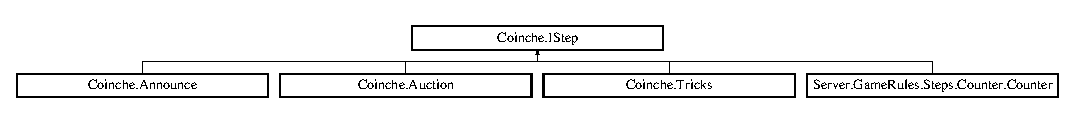
\includegraphics[height=1.081081cm]{interface_coinche_1_1_i_step}
\end{center}
\end{figure}
\subsection*{Public Member Functions}
\begin{DoxyCompactItemize}
\item 
void \hyperlink{interface_coinche_1_1_i_step_a764f20494a35e9b006c6495a38717e9a}{Reset} ()
\begin{DoxyCompactList}\small\item\em reset the step \end{DoxyCompactList}\item 
\hyperlink{class_coinche_1_1_tools_1_1_game_info}{Game\+Info} \hyperlink{interface_coinche_1_1_i_step_ada17a0e471c5afbc7e4f4acc434cdd76}{Prepare\+Step} (\hyperlink{class_coinche_1_1_player}{Player} player, int team\+Contract)
\begin{DoxyCompactList}\small\item\em prepare the players for the next step \end{DoxyCompactList}\item 
\hyperlink{class_coinche_1_1_tools_1_1_game_info}{Game\+Info} \hyperlink{interface_coinche_1_1_i_step_a1b410159a7988ae4e75154539715e7ba}{Do\+Step} (\hyperlink{class_coinche_1_1_player}{Player} player, string msg, Boolean all\+Assets, Boolean none\+Assets, Card\+Color color\+Bet, int first\+Player)
\begin{DoxyCompactList}\small\item\em rules of the current step applied with the players messages \end{DoxyCompactList}\item 
\hyperlink{class_coinche_1_1_tools_1_1_game_info}{Game\+Info} \hyperlink{interface_coinche_1_1_i_step_afc64813670860f5ee0829264751abc0a}{Invalid\+Turn} (\hyperlink{class_coinche_1_1_player}{Player} player)
\begin{DoxyCompactList}\small\item\em function called if it wasn\textquotesingle{}t the right turn to play \end{DoxyCompactList}\item 
string \hyperlink{interface_coinche_1_1_i_step_a86ef55b4c36ffa27f5fa18a10e9a61a0}{Step\+Over} ()
\begin{DoxyCompactList}\small\item\em function called when the step is over \end{DoxyCompactList}\end{DoxyCompactItemize}


\subsection{Detailed Description}
interface of each step 



\subsection{Member Function Documentation}
\mbox{\Hypertarget{interface_coinche_1_1_i_step_a1b410159a7988ae4e75154539715e7ba}\label{interface_coinche_1_1_i_step_a1b410159a7988ae4e75154539715e7ba}} 
\index{Coinche\+::\+I\+Step@{Coinche\+::\+I\+Step}!Do\+Step@{Do\+Step}}
\index{Do\+Step@{Do\+Step}!Coinche\+::\+I\+Step@{Coinche\+::\+I\+Step}}
\subsubsection{\texorpdfstring{Do\+Step()}{DoStep()}}
{\footnotesize\ttfamily \hyperlink{class_coinche_1_1_tools_1_1_game_info}{Game\+Info} Coinche.\+I\+Step.\+Do\+Step (\begin{DoxyParamCaption}\item[{\hyperlink{class_coinche_1_1_player}{Player}}]{player,  }\item[{string}]{msg,  }\item[{Boolean}]{all\+Assets,  }\item[{Boolean}]{none\+Assets,  }\item[{Card\+Color}]{color\+Bet,  }\item[{int}]{first\+Player }\end{DoxyParamCaption})}



rules of the current step applied with the players messages 


\begin{DoxyParams}{Parameters}
{\em player} & \\
\hline
{\em msg} & \\
\hline
{\em all\+Assets} & \\
\hline
{\em none\+Assets} & \\
\hline
{\em color\+Bet} & \\
\hline
{\em first\+Player} & \\
\hline
\end{DoxyParams}
\begin{DoxyReturn}{Returns}
a Game\+Info instance to tell players what happened
\end{DoxyReturn}


Implemented in \hyperlink{class_coinche_1_1_tricks_ae9cd4602740f7612010fac07af2997a8}{Coinche.\+Tricks}, \hyperlink{class_coinche_1_1_auction_ac43279f6867bd7896aee8e6ae504c472}{Coinche.\+Auction}, \hyperlink{class_server_1_1_game_rules_1_1_steps_1_1_counter_1_1_counter_aba717018db3366659fdb4ac302d19937}{Server.\+Game\+Rules.\+Steps.\+Counter.\+Counter}, and \hyperlink{class_coinche_1_1_announce_acf172bfff869b6e3f63ac4a18de63a55}{Coinche.\+Announce}.

\mbox{\Hypertarget{interface_coinche_1_1_i_step_afc64813670860f5ee0829264751abc0a}\label{interface_coinche_1_1_i_step_afc64813670860f5ee0829264751abc0a}} 
\index{Coinche\+::\+I\+Step@{Coinche\+::\+I\+Step}!Invalid\+Turn@{Invalid\+Turn}}
\index{Invalid\+Turn@{Invalid\+Turn}!Coinche\+::\+I\+Step@{Coinche\+::\+I\+Step}}
\subsubsection{\texorpdfstring{Invalid\+Turn()}{InvalidTurn()}}
{\footnotesize\ttfamily \hyperlink{class_coinche_1_1_tools_1_1_game_info}{Game\+Info} Coinche.\+I\+Step.\+Invalid\+Turn (\begin{DoxyParamCaption}\item[{\hyperlink{class_coinche_1_1_player}{Player}}]{player }\end{DoxyParamCaption})}



function called if it wasn\textquotesingle{}t the right turn to play 


\begin{DoxyParams}{Parameters}
{\em player} & \\
\hline
\end{DoxyParams}
\begin{DoxyReturn}{Returns}
a Game\+Info instance to inform the player it wasn\textquotesingle{}t his turn to play
\end{DoxyReturn}


Implemented in \hyperlink{class_coinche_1_1_tricks_a298a3f9c18af5a9e2ab7da3c7509075a}{Coinche.\+Tricks}, \hyperlink{class_coinche_1_1_auction_a00eba97a2289eb3bf7b2f4f7c84c8349}{Coinche.\+Auction}, \hyperlink{class_server_1_1_game_rules_1_1_steps_1_1_counter_1_1_counter_a81fc65a550bef61081dd1ec351b3bdaf}{Server.\+Game\+Rules.\+Steps.\+Counter.\+Counter}, and \hyperlink{class_coinche_1_1_announce_a778b04cb7ff3405d1a182e445a7c8f4c}{Coinche.\+Announce}.

\mbox{\Hypertarget{interface_coinche_1_1_i_step_ada17a0e471c5afbc7e4f4acc434cdd76}\label{interface_coinche_1_1_i_step_ada17a0e471c5afbc7e4f4acc434cdd76}} 
\index{Coinche\+::\+I\+Step@{Coinche\+::\+I\+Step}!Prepare\+Step@{Prepare\+Step}}
\index{Prepare\+Step@{Prepare\+Step}!Coinche\+::\+I\+Step@{Coinche\+::\+I\+Step}}
\subsubsection{\texorpdfstring{Prepare\+Step()}{PrepareStep()}}
{\footnotesize\ttfamily \hyperlink{class_coinche_1_1_tools_1_1_game_info}{Game\+Info} Coinche.\+I\+Step.\+Prepare\+Step (\begin{DoxyParamCaption}\item[{\hyperlink{class_coinche_1_1_player}{Player}}]{player,  }\item[{int}]{team\+Contract }\end{DoxyParamCaption})}



prepare the players for the next step 


\begin{DoxyParams}{Parameters}
{\em player} & \\
\hline
{\em team\+Contract} & \\
\hline
\end{DoxyParams}
\begin{DoxyReturn}{Returns}
infos to tell them what to do
\end{DoxyReturn}


Implemented in \hyperlink{class_coinche_1_1_tricks_a7d2fedfa7e574f3570d1be83943fa953}{Coinche.\+Tricks}, \hyperlink{class_coinche_1_1_auction_a9596ae8ce46f848244854d59c9bedadb}{Coinche.\+Auction}, \hyperlink{class_server_1_1_game_rules_1_1_steps_1_1_counter_1_1_counter_a84412648384fce7fea870e5e1e32bc3d}{Server.\+Game\+Rules.\+Steps.\+Counter.\+Counter}, and \hyperlink{class_coinche_1_1_announce_a24398cfbd8280465732c360858e72e13}{Coinche.\+Announce}.

\mbox{\Hypertarget{interface_coinche_1_1_i_step_a764f20494a35e9b006c6495a38717e9a}\label{interface_coinche_1_1_i_step_a764f20494a35e9b006c6495a38717e9a}} 
\index{Coinche\+::\+I\+Step@{Coinche\+::\+I\+Step}!Reset@{Reset}}
\index{Reset@{Reset}!Coinche\+::\+I\+Step@{Coinche\+::\+I\+Step}}
\subsubsection{\texorpdfstring{Reset()}{Reset()}}
{\footnotesize\ttfamily void Coinche.\+I\+Step.\+Reset (\begin{DoxyParamCaption}{ }\end{DoxyParamCaption})}



reset the step 



Implemented in \hyperlink{class_coinche_1_1_tricks_ade6668950abaf544373d90516821eab1}{Coinche.\+Tricks}, \hyperlink{class_coinche_1_1_auction_ae6b090721adfc333705f5f79ca9b462a}{Coinche.\+Auction}, \hyperlink{class_server_1_1_game_rules_1_1_steps_1_1_counter_1_1_counter_a7e681c51f20d2509e0b53dede3d73dc0}{Server.\+Game\+Rules.\+Steps.\+Counter.\+Counter}, and \hyperlink{class_coinche_1_1_announce_a0fddda733e5f081be1091b2c67279982}{Coinche.\+Announce}.

\mbox{\Hypertarget{interface_coinche_1_1_i_step_a86ef55b4c36ffa27f5fa18a10e9a61a0}\label{interface_coinche_1_1_i_step_a86ef55b4c36ffa27f5fa18a10e9a61a0}} 
\index{Coinche\+::\+I\+Step@{Coinche\+::\+I\+Step}!Step\+Over@{Step\+Over}}
\index{Step\+Over@{Step\+Over}!Coinche\+::\+I\+Step@{Coinche\+::\+I\+Step}}
\subsubsection{\texorpdfstring{Step\+Over()}{StepOver()}}
{\footnotesize\ttfamily string Coinche.\+I\+Step.\+Step\+Over (\begin{DoxyParamCaption}{ }\end{DoxyParamCaption})}



function called when the step is over 

\begin{DoxyReturn}{Returns}
a string to tell players the step is over
\end{DoxyReturn}


Implemented in \hyperlink{class_coinche_1_1_tricks_afa44486bcd0e3ce034330d8c0f0d36eb}{Coinche.\+Tricks}, \hyperlink{class_coinche_1_1_auction_ab1621fd742e17a9814671116d4d0682c}{Coinche.\+Auction}, \hyperlink{class_server_1_1_game_rules_1_1_steps_1_1_counter_1_1_counter_a75247ce8610225edadc753a432dd9c56}{Server.\+Game\+Rules.\+Steps.\+Counter.\+Counter}, and \hyperlink{class_coinche_1_1_announce_a3337d94429e31a70eb66ee0be3714e86}{Coinche.\+Announce}.



The documentation for this interface was generated from the following file\+:\begin{DoxyCompactItemize}
\item 
Server/\+Game\+Rules/\+Steps/I\+Step.\+cs\end{DoxyCompactItemize}

\hypertarget{class_coinche_1_1_tools_1_1_logger}{}\section{Coinche.\+Tools.\+Logger Class Reference}
\label{class_coinche_1_1_tools_1_1_logger}\index{Coinche.\+Tools.\+Logger@{Coinche.\+Tools.\+Logger}}


A simple \hyperlink{class_coinche_1_1_tools_1_1_logger}{Logger}.  


\subsection*{Public Member Functions}
\begin{DoxyCompactItemize}
\item 
\hyperlink{class_coinche_1_1_tools_1_1_logger_a2e3e986856697b6a0bd807e2ad491ecd}{Logger} (bool to\+File=true, bool append=false)
\begin{DoxyCompactList}\small\item\em Initialize a new instance of \hyperlink{class_coinche_1_1_tools_1_1_logger}{Logger} class. Log file will be created automatically if not yet exists, else it can be either a fresh new file or append to the existing file. Default is create a fresh new log file. \end{DoxyCompactList}\item 
void \hyperlink{class_coinche_1_1_tools_1_1_logger_a5e58c9a36a174cb4288591e7e94edf62}{Debug} (string text)
\begin{DoxyCompactList}\small\item\em Log a debug message \end{DoxyCompactList}\item 
void \hyperlink{class_coinche_1_1_tools_1_1_logger_a7f5ed11e008b28da749c517e39aaaff0}{Error} (string text)
\begin{DoxyCompactList}\small\item\em Log an error message \end{DoxyCompactList}\item 
void \hyperlink{class_coinche_1_1_tools_1_1_logger_a7a65b085b7e419cc629732be31ef7932}{Fatal} (string text)
\begin{DoxyCompactList}\small\item\em Log a fatal error message \end{DoxyCompactList}\item 
void \hyperlink{class_coinche_1_1_tools_1_1_logger_a49e8cfceab5aa777003d22cf33ecc4a1}{Info} (string text)
\begin{DoxyCompactList}\small\item\em Log an info message \end{DoxyCompactList}\item 
void \hyperlink{class_coinche_1_1_tools_1_1_logger_a8526ceb1f73b054f8bfd867bfe29f7c4}{Trace} (string text)
\begin{DoxyCompactList}\small\item\em Log a trace message \end{DoxyCompactList}\item 
void \hyperlink{class_coinche_1_1_tools_1_1_logger_aa2fb274fdb25913f1f43f16f36d9873c}{Warning} (string text)
\begin{DoxyCompactList}\small\item\em Log a waning message \end{DoxyCompactList}\end{DoxyCompactItemize}
\subsection*{Private Types}
\begin{DoxyCompactItemize}
\item 
enum \hyperlink{class_coinche_1_1_tools_1_1_logger_a92fb562053cc0a63b44bd10d2fb7d929}{Log\+Level} \{ \newline
{\bfseries T\+R\+A\+CE}, 
{\bfseries I\+N\+FO}, 
{\bfseries D\+E\+B\+UG}, 
{\bfseries W\+A\+R\+N\+I\+NG}, 
\newline
{\bfseries E\+R\+R\+OR}, 
{\bfseries F\+A\+T\+AL}
 \}\begin{DoxyCompactList}\small\item\em Supported log level \end{DoxyCompactList}
\end{DoxyCompactItemize}
\subsection*{Private Member Functions}
\begin{DoxyCompactItemize}
\item 
void \hyperlink{class_coinche_1_1_tools_1_1_logger_abe673ff15df5c49450232baf995bb74a}{Write\+Formatted\+Log} (\hyperlink{class_coinche_1_1_tools_1_1_logger_a92fb562053cc0a63b44bd10d2fb7d929}{Log\+Level} level, string text)
\begin{DoxyCompactList}\small\item\em Format a log message based on log level \end{DoxyCompactList}\item 
void \hyperlink{class_coinche_1_1_tools_1_1_logger_a92c8eb1380a72b2ac5cee18aec78cce8}{Write\+Line} (string text, bool append=true)
\begin{DoxyCompactList}\small\item\em Write a line of formatted log message into a log file \end{DoxyCompactList}\end{DoxyCompactItemize}
\subsection*{Private Attributes}
\begin{DoxyCompactItemize}
\item 
string \hyperlink{class_coinche_1_1_tools_1_1_logger_a3f00d015e0ea9978712a23abac8511b1}{Datetime\+Format}
\begin{DoxyCompactList}\small\item\em The datetime format. \end{DoxyCompactList}\item 
string \hyperlink{class_coinche_1_1_tools_1_1_logger_ab5055f470ac8880f10cf72f4ba6709f2}{Filename} = \char`\"{}\char`\"{}
\begin{DoxyCompactList}\small\item\em The filename. \end{DoxyCompactList}\end{DoxyCompactItemize}


\subsection{Detailed Description}
A simple \hyperlink{class_coinche_1_1_tools_1_1_logger}{Logger}. 



\subsection{Member Enumeration Documentation}
\mbox{\Hypertarget{class_coinche_1_1_tools_1_1_logger_a92fb562053cc0a63b44bd10d2fb7d929}\label{class_coinche_1_1_tools_1_1_logger_a92fb562053cc0a63b44bd10d2fb7d929}} 
\index{Coinche\+::\+Tools\+::\+Logger@{Coinche\+::\+Tools\+::\+Logger}!Log\+Level@{Log\+Level}}
\index{Log\+Level@{Log\+Level}!Coinche\+::\+Tools\+::\+Logger@{Coinche\+::\+Tools\+::\+Logger}}
\subsubsection{\texorpdfstring{Log\+Level}{LogLevel}}
{\footnotesize\ttfamily enum \hyperlink{class_coinche_1_1_tools_1_1_logger_a92fb562053cc0a63b44bd10d2fb7d929}{Coinche.\+Tools.\+Logger.\+Log\+Level}\hspace{0.3cm}{\ttfamily [strong]}, {\ttfamily [private]}}



Supported log level 



\subsection{Constructor \& Destructor Documentation}
\mbox{\Hypertarget{class_coinche_1_1_tools_1_1_logger_a2e3e986856697b6a0bd807e2ad491ecd}\label{class_coinche_1_1_tools_1_1_logger_a2e3e986856697b6a0bd807e2ad491ecd}} 
\index{Coinche\+::\+Tools\+::\+Logger@{Coinche\+::\+Tools\+::\+Logger}!Logger@{Logger}}
\index{Logger@{Logger}!Coinche\+::\+Tools\+::\+Logger@{Coinche\+::\+Tools\+::\+Logger}}
\subsubsection{\texorpdfstring{Logger()}{Logger()}}
{\footnotesize\ttfamily Coinche.\+Tools.\+Logger.\+Logger (\begin{DoxyParamCaption}\item[{bool}]{to\+File = {\ttfamily true},  }\item[{bool}]{append = {\ttfamily false} }\end{DoxyParamCaption})\hspace{0.3cm}{\ttfamily [inline]}}



Initialize a new instance of \hyperlink{class_coinche_1_1_tools_1_1_logger}{Logger} class. Log file will be created automatically if not yet exists, else it can be either a fresh new file or append to the existing file. Default is create a fresh new log file. 


\begin{DoxyParams}{Parameters}
{\em to\+File} & True to also log in a file, false otherwise\\
\hline
{\em append} & True to append to existing log file, False to overwrite and create new log file\\
\hline
\end{DoxyParams}


\subsection{Member Function Documentation}
\mbox{\Hypertarget{class_coinche_1_1_tools_1_1_logger_a5e58c9a36a174cb4288591e7e94edf62}\label{class_coinche_1_1_tools_1_1_logger_a5e58c9a36a174cb4288591e7e94edf62}} 
\index{Coinche\+::\+Tools\+::\+Logger@{Coinche\+::\+Tools\+::\+Logger}!Debug@{Debug}}
\index{Debug@{Debug}!Coinche\+::\+Tools\+::\+Logger@{Coinche\+::\+Tools\+::\+Logger}}
\subsubsection{\texorpdfstring{Debug()}{Debug()}}
{\footnotesize\ttfamily void Coinche.\+Tools.\+Logger.\+Debug (\begin{DoxyParamCaption}\item[{string}]{text }\end{DoxyParamCaption})\hspace{0.3cm}{\ttfamily [inline]}}



Log a debug message 


\begin{DoxyParams}{Parameters}
{\em text} & Message\\
\hline
\end{DoxyParams}
\mbox{\Hypertarget{class_coinche_1_1_tools_1_1_logger_a7f5ed11e008b28da749c517e39aaaff0}\label{class_coinche_1_1_tools_1_1_logger_a7f5ed11e008b28da749c517e39aaaff0}} 
\index{Coinche\+::\+Tools\+::\+Logger@{Coinche\+::\+Tools\+::\+Logger}!Error@{Error}}
\index{Error@{Error}!Coinche\+::\+Tools\+::\+Logger@{Coinche\+::\+Tools\+::\+Logger}}
\subsubsection{\texorpdfstring{Error()}{Error()}}
{\footnotesize\ttfamily void Coinche.\+Tools.\+Logger.\+Error (\begin{DoxyParamCaption}\item[{string}]{text }\end{DoxyParamCaption})\hspace{0.3cm}{\ttfamily [inline]}}



Log an error message 


\begin{DoxyParams}{Parameters}
{\em text} & Message\\
\hline
\end{DoxyParams}
\mbox{\Hypertarget{class_coinche_1_1_tools_1_1_logger_a7a65b085b7e419cc629732be31ef7932}\label{class_coinche_1_1_tools_1_1_logger_a7a65b085b7e419cc629732be31ef7932}} 
\index{Coinche\+::\+Tools\+::\+Logger@{Coinche\+::\+Tools\+::\+Logger}!Fatal@{Fatal}}
\index{Fatal@{Fatal}!Coinche\+::\+Tools\+::\+Logger@{Coinche\+::\+Tools\+::\+Logger}}
\subsubsection{\texorpdfstring{Fatal()}{Fatal()}}
{\footnotesize\ttfamily void Coinche.\+Tools.\+Logger.\+Fatal (\begin{DoxyParamCaption}\item[{string}]{text }\end{DoxyParamCaption})\hspace{0.3cm}{\ttfamily [inline]}}



Log a fatal error message 


\begin{DoxyParams}{Parameters}
{\em text} & Message\\
\hline
\end{DoxyParams}
\mbox{\Hypertarget{class_coinche_1_1_tools_1_1_logger_a49e8cfceab5aa777003d22cf33ecc4a1}\label{class_coinche_1_1_tools_1_1_logger_a49e8cfceab5aa777003d22cf33ecc4a1}} 
\index{Coinche\+::\+Tools\+::\+Logger@{Coinche\+::\+Tools\+::\+Logger}!Info@{Info}}
\index{Info@{Info}!Coinche\+::\+Tools\+::\+Logger@{Coinche\+::\+Tools\+::\+Logger}}
\subsubsection{\texorpdfstring{Info()}{Info()}}
{\footnotesize\ttfamily void Coinche.\+Tools.\+Logger.\+Info (\begin{DoxyParamCaption}\item[{string}]{text }\end{DoxyParamCaption})\hspace{0.3cm}{\ttfamily [inline]}}



Log an info message 


\begin{DoxyParams}{Parameters}
{\em text} & Message\\
\hline
\end{DoxyParams}
\mbox{\Hypertarget{class_coinche_1_1_tools_1_1_logger_a8526ceb1f73b054f8bfd867bfe29f7c4}\label{class_coinche_1_1_tools_1_1_logger_a8526ceb1f73b054f8bfd867bfe29f7c4}} 
\index{Coinche\+::\+Tools\+::\+Logger@{Coinche\+::\+Tools\+::\+Logger}!Trace@{Trace}}
\index{Trace@{Trace}!Coinche\+::\+Tools\+::\+Logger@{Coinche\+::\+Tools\+::\+Logger}}
\subsubsection{\texorpdfstring{Trace()}{Trace()}}
{\footnotesize\ttfamily void Coinche.\+Tools.\+Logger.\+Trace (\begin{DoxyParamCaption}\item[{string}]{text }\end{DoxyParamCaption})\hspace{0.3cm}{\ttfamily [inline]}}



Log a trace message 


\begin{DoxyParams}{Parameters}
{\em text} & Message\\
\hline
\end{DoxyParams}
\mbox{\Hypertarget{class_coinche_1_1_tools_1_1_logger_aa2fb274fdb25913f1f43f16f36d9873c}\label{class_coinche_1_1_tools_1_1_logger_aa2fb274fdb25913f1f43f16f36d9873c}} 
\index{Coinche\+::\+Tools\+::\+Logger@{Coinche\+::\+Tools\+::\+Logger}!Warning@{Warning}}
\index{Warning@{Warning}!Coinche\+::\+Tools\+::\+Logger@{Coinche\+::\+Tools\+::\+Logger}}
\subsubsection{\texorpdfstring{Warning()}{Warning()}}
{\footnotesize\ttfamily void Coinche.\+Tools.\+Logger.\+Warning (\begin{DoxyParamCaption}\item[{string}]{text }\end{DoxyParamCaption})\hspace{0.3cm}{\ttfamily [inline]}}



Log a waning message 


\begin{DoxyParams}{Parameters}
{\em text} & Message\\
\hline
\end{DoxyParams}
\mbox{\Hypertarget{class_coinche_1_1_tools_1_1_logger_abe673ff15df5c49450232baf995bb74a}\label{class_coinche_1_1_tools_1_1_logger_abe673ff15df5c49450232baf995bb74a}} 
\index{Coinche\+::\+Tools\+::\+Logger@{Coinche\+::\+Tools\+::\+Logger}!Write\+Formatted\+Log@{Write\+Formatted\+Log}}
\index{Write\+Formatted\+Log@{Write\+Formatted\+Log}!Coinche\+::\+Tools\+::\+Logger@{Coinche\+::\+Tools\+::\+Logger}}
\subsubsection{\texorpdfstring{Write\+Formatted\+Log()}{WriteFormattedLog()}}
{\footnotesize\ttfamily void Coinche.\+Tools.\+Logger.\+Write\+Formatted\+Log (\begin{DoxyParamCaption}\item[{\hyperlink{class_coinche_1_1_tools_1_1_logger_a92fb562053cc0a63b44bd10d2fb7d929}{Log\+Level}}]{level,  }\item[{string}]{text }\end{DoxyParamCaption})\hspace{0.3cm}{\ttfamily [inline]}, {\ttfamily [private]}}



Format a log message based on log level 


\begin{DoxyParams}{Parameters}
{\em level} & Log level\\
\hline
{\em text} & Log message\\
\hline
\end{DoxyParams}
\mbox{\Hypertarget{class_coinche_1_1_tools_1_1_logger_a92c8eb1380a72b2ac5cee18aec78cce8}\label{class_coinche_1_1_tools_1_1_logger_a92c8eb1380a72b2ac5cee18aec78cce8}} 
\index{Coinche\+::\+Tools\+::\+Logger@{Coinche\+::\+Tools\+::\+Logger}!Write\+Line@{Write\+Line}}
\index{Write\+Line@{Write\+Line}!Coinche\+::\+Tools\+::\+Logger@{Coinche\+::\+Tools\+::\+Logger}}
\subsubsection{\texorpdfstring{Write\+Line()}{WriteLine()}}
{\footnotesize\ttfamily void Coinche.\+Tools.\+Logger.\+Write\+Line (\begin{DoxyParamCaption}\item[{string}]{text,  }\item[{bool}]{append = {\ttfamily true} }\end{DoxyParamCaption})\hspace{0.3cm}{\ttfamily [inline]}, {\ttfamily [private]}}



Write a line of formatted log message into a log file 


\begin{DoxyParams}{Parameters}
{\em text} & Formatted log message\\
\hline
{\em append} & True to append, False to overwrite the file\\
\hline
\end{DoxyParams}

\begin{DoxyExceptions}{Exceptions}
{\em System.\+I\+O.\+I\+O\+Exception} & \\
\hline
\end{DoxyExceptions}


\subsection{Member Data Documentation}
\mbox{\Hypertarget{class_coinche_1_1_tools_1_1_logger_a3f00d015e0ea9978712a23abac8511b1}\label{class_coinche_1_1_tools_1_1_logger_a3f00d015e0ea9978712a23abac8511b1}} 
\index{Coinche\+::\+Tools\+::\+Logger@{Coinche\+::\+Tools\+::\+Logger}!Datetime\+Format@{Datetime\+Format}}
\index{Datetime\+Format@{Datetime\+Format}!Coinche\+::\+Tools\+::\+Logger@{Coinche\+::\+Tools\+::\+Logger}}
\subsubsection{\texorpdfstring{Datetime\+Format}{DatetimeFormat}}
{\footnotesize\ttfamily string Coinche.\+Tools.\+Logger.\+Datetime\+Format\hspace{0.3cm}{\ttfamily [private]}}



The datetime format. 

\mbox{\Hypertarget{class_coinche_1_1_tools_1_1_logger_ab5055f470ac8880f10cf72f4ba6709f2}\label{class_coinche_1_1_tools_1_1_logger_ab5055f470ac8880f10cf72f4ba6709f2}} 
\index{Coinche\+::\+Tools\+::\+Logger@{Coinche\+::\+Tools\+::\+Logger}!Filename@{Filename}}
\index{Filename@{Filename}!Coinche\+::\+Tools\+::\+Logger@{Coinche\+::\+Tools\+::\+Logger}}
\subsubsection{\texorpdfstring{Filename}{Filename}}
{\footnotesize\ttfamily string Coinche.\+Tools.\+Logger.\+Filename = \char`\"{}\char`\"{}\hspace{0.3cm}{\ttfamily [private]}}



The filename. 



The documentation for this class was generated from the following file\+:\begin{DoxyCompactItemize}
\item 
Server/\+Tools/Logger.\+cs\end{DoxyCompactItemize}

\hypertarget{class_coinche_1_1_player}{}\section{Coinche.\+Player Class Reference}
\label{class_coinche_1_1_player}\index{Coinche.\+Player@{Coinche.\+Player}}


class defining a player  


\subsection*{Public Member Functions}
\begin{DoxyCompactItemize}
\item 
\hyperlink{class_coinche_1_1_player_a2111dfa81103a51e186b77dd90b73c22}{Player} (int \+\_\+id)
\begin{DoxyCompactList}\small\item\em Initialize the player from its id \end{DoxyCompactList}\item 
void \hyperlink{class_coinche_1_1_player_afc5c66bf2caf32ea6a55fd2db27b6ae6}{Display\+Hand} ()
\begin{DoxyCompactList}\small\item\em Display the player\textquotesingle{}s hand \end{DoxyCompactList}\item 
Boolean \hyperlink{class_coinche_1_1_player_a20320a851740a462825fa0098a942834}{Got\+Color\+In\+Hand} (Card\+Color c)
\begin{DoxyCompactList}\small\item\em Check if the player has the given color in his hand \end{DoxyCompactList}\item 
string \hyperlink{class_coinche_1_1_player_a837c604aef1f5845a0728b7b53facc94}{Get\+Hand\+As\+String} ()
\begin{DoxyCompactList}\small\item\em get the hand has a string to inform players \end{DoxyCompactList}\item 
\hyperlink{class_coinche_1_1_card}{Card} \hyperlink{class_coinche_1_1_player_a3d79efe6f0971335edaaa2a0039aba00}{Play\+Card} (\hyperlink{class_coinche_1_1_card}{Card}\mbox{[}$\,$\mbox{]} game\+Board, Card\+Color color\+Bet, Boolean all\+Assets, Boolean none\+Assets, int first\+Player, String card\+To\+Play)
\begin{DoxyCompactList}\small\item\em play a card if valid \end{DoxyCompactList}\end{DoxyCompactItemize}
\subsection*{Properties}
\begin{DoxyCompactItemize}
\item 
int \hyperlink{class_coinche_1_1_player_af200e29b3845a8610f019f93e9b49caa}{id}\hspace{0.3cm}{\ttfamily  \mbox{[}get, private set\mbox{]}}
\begin{DoxyCompactList}\small\item\em id of a player \end{DoxyCompactList}\item 
List$<$ \hyperlink{class_coinche_1_1_card}{Card} $>$ \hyperlink{class_coinche_1_1_player_a22527d95a53a30c571986e354ebc63f8}{Hand}\hspace{0.3cm}{\ttfamily  \mbox{[}get, set\mbox{]}}
\begin{DoxyCompactList}\small\item\em cards the player have in his hand \end{DoxyCompactList}\end{DoxyCompactItemize}
\subsection*{Private Member Functions}
\begin{DoxyCompactItemize}
\item 
Boolean \hyperlink{class_coinche_1_1_player_adfb688665d8b3e6493e4832d32fbaf1d}{Card\+Is\+Valid} (\hyperlink{class_coinche_1_1_card}{Card} c, \hyperlink{class_coinche_1_1_card}{Card}\mbox{[}$\,$\mbox{]} game\+Board, Card\+Color color\+Bet, Boolean all\+Assets, Boolean none\+Assets, int first\+Player)
\begin{DoxyCompactList}\small\item\em check if the card to play is valid \end{DoxyCompactList}\item 
Boolean \hyperlink{class_coinche_1_1_player_a8f04f1fb2e697163b2728450c3e24f31}{Got\+Better\+In\+Hand} (\hyperlink{class_coinche_1_1_card}{Card}\mbox{[}$\,$\mbox{]} game\+Board, Card\+Color color\+Bet)
\begin{DoxyCompactList}\small\item\em check if the player has a better card of the given color in hand \end{DoxyCompactList}\item 
Boolean \hyperlink{class_coinche_1_1_player_a93948ebdc512c349d00390d44272bc14}{Card\+Is\+Weaker\+Than\+Game\+Board} (\hyperlink{class_coinche_1_1_card}{Card} c, \hyperlink{class_coinche_1_1_card}{Card}\mbox{[}$\,$\mbox{]} game\+Board, Card\+Color color\+Bet)
\begin{DoxyCompactList}\small\item\em check if the card is weaker than the ones on the board \end{DoxyCompactList}\end{DoxyCompactItemize}


\subsection{Detailed Description}
class defining a player 



\subsection{Constructor \& Destructor Documentation}
\mbox{\Hypertarget{class_coinche_1_1_player_a2111dfa81103a51e186b77dd90b73c22}\label{class_coinche_1_1_player_a2111dfa81103a51e186b77dd90b73c22}} 
\index{Coinche\+::\+Player@{Coinche\+::\+Player}!Player@{Player}}
\index{Player@{Player}!Coinche\+::\+Player@{Coinche\+::\+Player}}
\subsubsection{\texorpdfstring{Player()}{Player()}}
{\footnotesize\ttfamily Coinche.\+Player.\+Player (\begin{DoxyParamCaption}\item[{int}]{\+\_\+id }\end{DoxyParamCaption})\hspace{0.3cm}{\ttfamily [inline]}}



Initialize the player from its id 


\begin{DoxyParams}{Parameters}
{\em \+\_\+id} & \\
\hline
\end{DoxyParams}


\subsection{Member Function Documentation}
\mbox{\Hypertarget{class_coinche_1_1_player_adfb688665d8b3e6493e4832d32fbaf1d}\label{class_coinche_1_1_player_adfb688665d8b3e6493e4832d32fbaf1d}} 
\index{Coinche\+::\+Player@{Coinche\+::\+Player}!Card\+Is\+Valid@{Card\+Is\+Valid}}
\index{Card\+Is\+Valid@{Card\+Is\+Valid}!Coinche\+::\+Player@{Coinche\+::\+Player}}
\subsubsection{\texorpdfstring{Card\+Is\+Valid()}{CardIsValid()}}
{\footnotesize\ttfamily Boolean Coinche.\+Player.\+Card\+Is\+Valid (\begin{DoxyParamCaption}\item[{\hyperlink{class_coinche_1_1_card}{Card}}]{c,  }\item[{\hyperlink{class_coinche_1_1_card}{Card} \mbox{[}$\,$\mbox{]}}]{game\+Board,  }\item[{Card\+Color}]{color\+Bet,  }\item[{Boolean}]{all\+Assets,  }\item[{Boolean}]{none\+Assets,  }\item[{int}]{first\+Player }\end{DoxyParamCaption})\hspace{0.3cm}{\ttfamily [inline]}, {\ttfamily [private]}}



check if the card to play is valid 


\begin{DoxyParams}{Parameters}
{\em c} & \\
\hline
{\em game\+Board} & \\
\hline
{\em color\+Bet} & \\
\hline
{\em all\+Assets} & \\
\hline
{\em none\+Assets} & \\
\hline
{\em first\+Player} & \\
\hline
\end{DoxyParams}
\begin{DoxyReturn}{Returns}
true if valid else false
\end{DoxyReturn}
\mbox{\Hypertarget{class_coinche_1_1_player_a93948ebdc512c349d00390d44272bc14}\label{class_coinche_1_1_player_a93948ebdc512c349d00390d44272bc14}} 
\index{Coinche\+::\+Player@{Coinche\+::\+Player}!Card\+Is\+Weaker\+Than\+Game\+Board@{Card\+Is\+Weaker\+Than\+Game\+Board}}
\index{Card\+Is\+Weaker\+Than\+Game\+Board@{Card\+Is\+Weaker\+Than\+Game\+Board}!Coinche\+::\+Player@{Coinche\+::\+Player}}
\subsubsection{\texorpdfstring{Card\+Is\+Weaker\+Than\+Game\+Board()}{CardIsWeakerThanGameBoard()}}
{\footnotesize\ttfamily Boolean Coinche.\+Player.\+Card\+Is\+Weaker\+Than\+Game\+Board (\begin{DoxyParamCaption}\item[{\hyperlink{class_coinche_1_1_card}{Card}}]{c,  }\item[{\hyperlink{class_coinche_1_1_card}{Card} \mbox{[}$\,$\mbox{]}}]{game\+Board,  }\item[{Card\+Color}]{color\+Bet }\end{DoxyParamCaption})\hspace{0.3cm}{\ttfamily [inline]}, {\ttfamily [private]}}



check if the card is weaker than the ones on the board 


\begin{DoxyParams}{Parameters}
{\em c} & \\
\hline
{\em game\+Board} & \\
\hline
{\em color\+Bet} & \\
\hline
\end{DoxyParams}
\begin{DoxyReturn}{Returns}
returns true if the card is weaker else false
\end{DoxyReturn}
\mbox{\Hypertarget{class_coinche_1_1_player_afc5c66bf2caf32ea6a55fd2db27b6ae6}\label{class_coinche_1_1_player_afc5c66bf2caf32ea6a55fd2db27b6ae6}} 
\index{Coinche\+::\+Player@{Coinche\+::\+Player}!Display\+Hand@{Display\+Hand}}
\index{Display\+Hand@{Display\+Hand}!Coinche\+::\+Player@{Coinche\+::\+Player}}
\subsubsection{\texorpdfstring{Display\+Hand()}{DisplayHand()}}
{\footnotesize\ttfamily void Coinche.\+Player.\+Display\+Hand (\begin{DoxyParamCaption}{ }\end{DoxyParamCaption})\hspace{0.3cm}{\ttfamily [inline]}}



Display the player\textquotesingle{}s hand 

\mbox{\Hypertarget{class_coinche_1_1_player_a837c604aef1f5845a0728b7b53facc94}\label{class_coinche_1_1_player_a837c604aef1f5845a0728b7b53facc94}} 
\index{Coinche\+::\+Player@{Coinche\+::\+Player}!Get\+Hand\+As\+String@{Get\+Hand\+As\+String}}
\index{Get\+Hand\+As\+String@{Get\+Hand\+As\+String}!Coinche\+::\+Player@{Coinche\+::\+Player}}
\subsubsection{\texorpdfstring{Get\+Hand\+As\+String()}{GetHandAsString()}}
{\footnotesize\ttfamily string Coinche.\+Player.\+Get\+Hand\+As\+String (\begin{DoxyParamCaption}{ }\end{DoxyParamCaption})\hspace{0.3cm}{\ttfamily [inline]}}



get the hand has a string to inform players 

\begin{DoxyReturn}{Returns}
the cards in the player\textquotesingle{}s hand
\end{DoxyReturn}
\mbox{\Hypertarget{class_coinche_1_1_player_a8f04f1fb2e697163b2728450c3e24f31}\label{class_coinche_1_1_player_a8f04f1fb2e697163b2728450c3e24f31}} 
\index{Coinche\+::\+Player@{Coinche\+::\+Player}!Got\+Better\+In\+Hand@{Got\+Better\+In\+Hand}}
\index{Got\+Better\+In\+Hand@{Got\+Better\+In\+Hand}!Coinche\+::\+Player@{Coinche\+::\+Player}}
\subsubsection{\texorpdfstring{Got\+Better\+In\+Hand()}{GotBetterInHand()}}
{\footnotesize\ttfamily Boolean Coinche.\+Player.\+Got\+Better\+In\+Hand (\begin{DoxyParamCaption}\item[{\hyperlink{class_coinche_1_1_card}{Card} \mbox{[}$\,$\mbox{]}}]{game\+Board,  }\item[{Card\+Color}]{color\+Bet }\end{DoxyParamCaption})\hspace{0.3cm}{\ttfamily [inline]}, {\ttfamily [private]}}



check if the player has a better card of the given color in hand 


\begin{DoxyParams}{Parameters}
{\em game\+Board} & \\
\hline
{\em color\+Bet} & \\
\hline
\end{DoxyParams}
\begin{DoxyReturn}{Returns}
return true if he got better else false
\end{DoxyReturn}
\mbox{\Hypertarget{class_coinche_1_1_player_a20320a851740a462825fa0098a942834}\label{class_coinche_1_1_player_a20320a851740a462825fa0098a942834}} 
\index{Coinche\+::\+Player@{Coinche\+::\+Player}!Got\+Color\+In\+Hand@{Got\+Color\+In\+Hand}}
\index{Got\+Color\+In\+Hand@{Got\+Color\+In\+Hand}!Coinche\+::\+Player@{Coinche\+::\+Player}}
\subsubsection{\texorpdfstring{Got\+Color\+In\+Hand()}{GotColorInHand()}}
{\footnotesize\ttfamily Boolean Coinche.\+Player.\+Got\+Color\+In\+Hand (\begin{DoxyParamCaption}\item[{Card\+Color}]{c }\end{DoxyParamCaption})\hspace{0.3cm}{\ttfamily [inline]}}



Check if the player has the given color in his hand 


\begin{DoxyParams}{Parameters}
{\em c} & \\
\hline
\end{DoxyParams}
\begin{DoxyReturn}{Returns}
true if he has it else false
\end{DoxyReturn}
\mbox{\Hypertarget{class_coinche_1_1_player_a3d79efe6f0971335edaaa2a0039aba00}\label{class_coinche_1_1_player_a3d79efe6f0971335edaaa2a0039aba00}} 
\index{Coinche\+::\+Player@{Coinche\+::\+Player}!Play\+Card@{Play\+Card}}
\index{Play\+Card@{Play\+Card}!Coinche\+::\+Player@{Coinche\+::\+Player}}
\subsubsection{\texorpdfstring{Play\+Card()}{PlayCard()}}
{\footnotesize\ttfamily \hyperlink{class_coinche_1_1_card}{Card} Coinche.\+Player.\+Play\+Card (\begin{DoxyParamCaption}\item[{\hyperlink{class_coinche_1_1_card}{Card} \mbox{[}$\,$\mbox{]}}]{game\+Board,  }\item[{Card\+Color}]{color\+Bet,  }\item[{Boolean}]{all\+Assets,  }\item[{Boolean}]{none\+Assets,  }\item[{int}]{first\+Player,  }\item[{String}]{card\+To\+Play }\end{DoxyParamCaption})\hspace{0.3cm}{\ttfamily [inline]}}



play a card if valid 


\begin{DoxyParams}{Parameters}
{\em game\+Board} & \\
\hline
{\em color\+Bet} & \\
\hline
{\em all\+Assets} & \\
\hline
{\em none\+Assets} & \\
\hline
{\em first\+Player} & \\
\hline
{\em card\+To\+Play} & \\
\hline
\end{DoxyParams}
\begin{DoxyReturn}{Returns}
return the card played or null
\end{DoxyReturn}


\subsection{Property Documentation}
\mbox{\Hypertarget{class_coinche_1_1_player_a22527d95a53a30c571986e354ebc63f8}\label{class_coinche_1_1_player_a22527d95a53a30c571986e354ebc63f8}} 
\index{Coinche\+::\+Player@{Coinche\+::\+Player}!Hand@{Hand}}
\index{Hand@{Hand}!Coinche\+::\+Player@{Coinche\+::\+Player}}
\subsubsection{\texorpdfstring{Hand}{Hand}}
{\footnotesize\ttfamily List$<$\hyperlink{class_coinche_1_1_card}{Card}$>$ Coinche.\+Player.\+Hand\hspace{0.3cm}{\ttfamily [get]}, {\ttfamily [set]}}



cards the player have in his hand 

\mbox{\Hypertarget{class_coinche_1_1_player_af200e29b3845a8610f019f93e9b49caa}\label{class_coinche_1_1_player_af200e29b3845a8610f019f93e9b49caa}} 
\index{Coinche\+::\+Player@{Coinche\+::\+Player}!id@{id}}
\index{id@{id}!Coinche\+::\+Player@{Coinche\+::\+Player}}
\subsubsection{\texorpdfstring{id}{id}}
{\footnotesize\ttfamily int Coinche.\+Player.\+id\hspace{0.3cm}{\ttfamily [get]}, {\ttfamily [private set]}}



id of a player 



The documentation for this class was generated from the following file\+:\begin{DoxyCompactItemize}
\item 
Server/\+Game\+Rules/Player.\+cs\end{DoxyCompactItemize}

\hypertarget{class_coinche_1_1_server_1_1_program}{}\section{Coinche.\+Server.\+Program Class Reference}
\label{class_coinche_1_1_server_1_1_program}\index{Coinche.\+Server.\+Program@{Coinche.\+Server.\+Program}}


J\+Coinche \hyperlink{namespace_coinche_1_1_server}{Server} main class  


\subsection*{Static Private Member Functions}
\begin{DoxyCompactItemize}
\item 
static async Task \hyperlink{class_coinche_1_1_server_1_1_program_a376ce464c8f3725aa59134c9589a4ceb}{Run\+Server\+Async} (I\+P\+Address addr, short port)
\begin{DoxyCompactList}\small\item\em Runs the server async. \end{DoxyCompactList}\item 
static void \hyperlink{class_coinche_1_1_server_1_1_program_a48a23f5d3c3de01732d7f492c4e55e01}{Main} (String\mbox{[}$\,$\mbox{]} args)
\begin{DoxyCompactList}\small\item\em The entry point of the program, where the program control starts and ends. \end{DoxyCompactList}\end{DoxyCompactItemize}


\subsection{Detailed Description}
J\+Coinche \hyperlink{namespace_coinche_1_1_server}{Server} main class 



\subsection{Member Function Documentation}
\mbox{\Hypertarget{class_coinche_1_1_server_1_1_program_a48a23f5d3c3de01732d7f492c4e55e01}\label{class_coinche_1_1_server_1_1_program_a48a23f5d3c3de01732d7f492c4e55e01}} 
\index{Coinche\+::\+Server\+::\+Program@{Coinche\+::\+Server\+::\+Program}!Main@{Main}}
\index{Main@{Main}!Coinche\+::\+Server\+::\+Program@{Coinche\+::\+Server\+::\+Program}}
\subsubsection{\texorpdfstring{Main()}{Main()}}
{\footnotesize\ttfamily static void Coinche.\+Server.\+Program.\+Main (\begin{DoxyParamCaption}\item[{String \mbox{[}$\,$\mbox{]}}]{args }\end{DoxyParamCaption})\hspace{0.3cm}{\ttfamily [inline]}, {\ttfamily [static]}, {\ttfamily [private]}}



The entry point of the program, where the program control starts and ends. 


\begin{DoxyParams}{Parameters}
{\em args} & The command-\/line arguments.\\
\hline
\end{DoxyParams}
\begin{DoxyReturn}{Returns}
The exit code that is given to the operating system after the program ends.
\end{DoxyReturn}
\mbox{\Hypertarget{class_coinche_1_1_server_1_1_program_a376ce464c8f3725aa59134c9589a4ceb}\label{class_coinche_1_1_server_1_1_program_a376ce464c8f3725aa59134c9589a4ceb}} 
\index{Coinche\+::\+Server\+::\+Program@{Coinche\+::\+Server\+::\+Program}!Run\+Server\+Async@{Run\+Server\+Async}}
\index{Run\+Server\+Async@{Run\+Server\+Async}!Coinche\+::\+Server\+::\+Program@{Coinche\+::\+Server\+::\+Program}}
\subsubsection{\texorpdfstring{Run\+Server\+Async()}{RunServerAsync()}}
{\footnotesize\ttfamily static async Task Coinche.\+Server.\+Program.\+Run\+Server\+Async (\begin{DoxyParamCaption}\item[{I\+P\+Address}]{addr,  }\item[{short}]{port }\end{DoxyParamCaption})\hspace{0.3cm}{\ttfamily [inline]}, {\ttfamily [static]}, {\ttfamily [private]}}



Runs the server async. 

\begin{DoxyReturn}{Returns}
The server async.
\end{DoxyReturn}


The documentation for this class was generated from the following file\+:\begin{DoxyCompactItemize}
\item 
Server/\+Core/Program.\+cs\end{DoxyCompactItemize}

\hypertarget{class_coinche_1_1_client_1_1_program}{}\section{Coinche.\+Client.\+Program Class Reference}
\label{class_coinche_1_1_client_1_1_program}\index{Coinche.\+Client.\+Program@{Coinche.\+Client.\+Program}}


Jcoinche \hyperlink{namespace_coinche_1_1_client}{Client} Main \hyperlink{class_coinche_1_1_client_1_1_program}{Program}  


\subsection*{Static Public Member Functions}
\begin{DoxyCompactItemize}
\item 
static int \hyperlink{class_coinche_1_1_client_1_1_program_a4017f65cee201ce2c210a4abc290c663}{Main} (String\mbox{[}$\,$\mbox{]} args)
\begin{DoxyCompactList}\small\item\em The entry point of the program, where the program control starts and ends. \end{DoxyCompactList}\end{DoxyCompactItemize}
\subsection*{Static Private Member Functions}
\begin{DoxyCompactItemize}
\item 
static async Task \hyperlink{class_coinche_1_1_client_1_1_program_a748963e969bfd9e466f58422f39bc1b8}{Run\+Client\+Async} (I\+P\+Address addr, short port)
\begin{DoxyCompactList}\small\item\em Runs the client async. \end{DoxyCompactList}\end{DoxyCompactItemize}


\subsection{Detailed Description}
Jcoinche \hyperlink{namespace_coinche_1_1_client}{Client} Main \hyperlink{class_coinche_1_1_client_1_1_program}{Program} 



\subsection{Member Function Documentation}
\mbox{\Hypertarget{class_coinche_1_1_client_1_1_program_a4017f65cee201ce2c210a4abc290c663}\label{class_coinche_1_1_client_1_1_program_a4017f65cee201ce2c210a4abc290c663}} 
\index{Coinche\+::\+Client\+::\+Program@{Coinche\+::\+Client\+::\+Program}!Main@{Main}}
\index{Main@{Main}!Coinche\+::\+Client\+::\+Program@{Coinche\+::\+Client\+::\+Program}}
\subsubsection{\texorpdfstring{Main()}{Main()}}
{\footnotesize\ttfamily static int Coinche.\+Client.\+Program.\+Main (\begin{DoxyParamCaption}\item[{String \mbox{[}$\,$\mbox{]}}]{args }\end{DoxyParamCaption})\hspace{0.3cm}{\ttfamily [inline]}, {\ttfamily [static]}}



The entry point of the program, where the program control starts and ends. 


\begin{DoxyParams}{Parameters}
{\em args} & The command-\/line arguments.\\
\hline
\end{DoxyParams}
\begin{DoxyReturn}{Returns}
The exit code that is given to the operating system after the program ends.
\end{DoxyReturn}
\mbox{\Hypertarget{class_coinche_1_1_client_1_1_program_a748963e969bfd9e466f58422f39bc1b8}\label{class_coinche_1_1_client_1_1_program_a748963e969bfd9e466f58422f39bc1b8}} 
\index{Coinche\+::\+Client\+::\+Program@{Coinche\+::\+Client\+::\+Program}!Run\+Client\+Async@{Run\+Client\+Async}}
\index{Run\+Client\+Async@{Run\+Client\+Async}!Coinche\+::\+Client\+::\+Program@{Coinche\+::\+Client\+::\+Program}}
\subsubsection{\texorpdfstring{Run\+Client\+Async()}{RunClientAsync()}}
{\footnotesize\ttfamily static async Task Coinche.\+Client.\+Program.\+Run\+Client\+Async (\begin{DoxyParamCaption}\item[{I\+P\+Address}]{addr,  }\item[{short}]{port }\end{DoxyParamCaption})\hspace{0.3cm}{\ttfamily [inline]}, {\ttfamily [static]}, {\ttfamily [private]}}



Runs the client async. 

\begin{DoxyReturn}{Returns}
The client async.
\end{DoxyReturn}

\begin{DoxyParams}{Parameters}
{\em addr} & Address.\\
\hline
{\em port} & Port.\\
\hline
\end{DoxyParams}


The documentation for this class was generated from the following file\+:\begin{DoxyCompactItemize}
\item 
Client/\+Core/Program.\+cs\end{DoxyCompactItemize}

\hypertarget{class_coinche_1_1_steps}{}\section{Coinche.\+Steps Class Reference}
\label{class_coinche_1_1_steps}\index{Coinche.\+Steps@{Coinche.\+Steps}}


class in which there is all the steps of the game  


\subsection*{Public Member Functions}
\begin{DoxyCompactItemize}
\item 
\hyperlink{class_coinche_1_1_steps_a7dd11c324b2f7fe132a621970681a02d}{Steps} ()
\begin{DoxyCompactList}\small\item\em simple constructor \end{DoxyCompactList}\item 
void \hyperlink{class_coinche_1_1_steps_a6d7bee3e38106357f9dd82e42e75c94a}{Reset} ()
\begin{DoxyCompactList}\small\item\em reinitialize the steps for a new round \end{DoxyCompactList}\item 
\hyperlink{class_coinche_1_1_tools_1_1_game_info}{Game\+Info} \hyperlink{class_coinche_1_1_steps_ab92a1baf655d05a75cd0b9842f4b5a36}{Prepare\+Next\+Step} (\hyperlink{class_coinche_1_1_player}{Player} player, int team\+Contract)
\begin{DoxyCompactList}\small\item\em get the infos for the next step \end{DoxyCompactList}\item 
\hyperlink{class_coinche_1_1_tools_1_1_game_info}{Game\+Info} \hyperlink{class_coinche_1_1_steps_abaae452876448173aab048ebadb2b529}{Do\+Next\+Step} (\hyperlink{class_coinche_1_1_player}{Player} player, string msg, Boolean all\+Assets, Boolean none\+Assets, Card\+Color color\+Bet, int first\+Player)
\begin{DoxyCompactList}\small\item\em send the message a player wants to play to the current step \end{DoxyCompactList}\item 
\hyperlink{class_coinche_1_1_tools_1_1_game_info}{Game\+Info} \hyperlink{class_coinche_1_1_steps_a1446affd62b6aaecafaf4959cf6f829a}{Invalid\+Turn} (\hyperlink{class_coinche_1_1_player}{Player} player)
\begin{DoxyCompactList}\small\item\em function called if it wasn\textquotesingle{}t the right turn to play \end{DoxyCompactList}\end{DoxyCompactItemize}
\subsection*{Properties}
\begin{DoxyCompactItemize}
\item 
Step \hyperlink{class_coinche_1_1_steps_a03916f3a20f2b181afefc14b14663eb3}{Current\+Step}\hspace{0.3cm}{\ttfamily  \mbox{[}get, set\mbox{]}}
\begin{DoxyCompactList}\small\item\em the current step \end{DoxyCompactList}\end{DoxyCompactItemize}
\subsection*{Private Attributes}
\begin{DoxyCompactItemize}
\item 
List$<$ \hyperlink{interface_coinche_1_1_i_step}{I\+Step} $>$ \hyperlink{class_coinche_1_1_steps_ae755de9f482239900819fc7d90608b55}{Round\+Steps}
\begin{DoxyCompactList}\small\item\em list of all the steps \end{DoxyCompactList}\end{DoxyCompactItemize}


\subsection{Detailed Description}
class in which there is all the steps of the game 



\subsection{Constructor \& Destructor Documentation}
\mbox{\Hypertarget{class_coinche_1_1_steps_a7dd11c324b2f7fe132a621970681a02d}\label{class_coinche_1_1_steps_a7dd11c324b2f7fe132a621970681a02d}} 
\index{Coinche\+::\+Steps@{Coinche\+::\+Steps}!Steps@{Steps}}
\index{Steps@{Steps}!Coinche\+::\+Steps@{Coinche\+::\+Steps}}
\subsubsection{\texorpdfstring{Steps()}{Steps()}}
{\footnotesize\ttfamily Coinche.\+Steps.\+Steps (\begin{DoxyParamCaption}{ }\end{DoxyParamCaption})\hspace{0.3cm}{\ttfamily [inline]}}



simple constructor 



\subsection{Member Function Documentation}
\mbox{\Hypertarget{class_coinche_1_1_steps_abaae452876448173aab048ebadb2b529}\label{class_coinche_1_1_steps_abaae452876448173aab048ebadb2b529}} 
\index{Coinche\+::\+Steps@{Coinche\+::\+Steps}!Do\+Next\+Step@{Do\+Next\+Step}}
\index{Do\+Next\+Step@{Do\+Next\+Step}!Coinche\+::\+Steps@{Coinche\+::\+Steps}}
\subsubsection{\texorpdfstring{Do\+Next\+Step()}{DoNextStep()}}
{\footnotesize\ttfamily \hyperlink{class_coinche_1_1_tools_1_1_game_info}{Game\+Info} Coinche.\+Steps.\+Do\+Next\+Step (\begin{DoxyParamCaption}\item[{\hyperlink{class_coinche_1_1_player}{Player}}]{player,  }\item[{string}]{msg,  }\item[{Boolean}]{all\+Assets,  }\item[{Boolean}]{none\+Assets,  }\item[{Card\+Color}]{color\+Bet,  }\item[{int}]{first\+Player }\end{DoxyParamCaption})\hspace{0.3cm}{\ttfamily [inline]}}



send the message a player wants to play to the current step 


\begin{DoxyParams}{Parameters}
{\em player} & \\
\hline
{\em msg} & \\
\hline
{\em all\+Assets} & \\
\hline
{\em none\+Assets} & \\
\hline
{\em color\+Bet} & \\
\hline
{\em first\+Player} & \\
\hline
\end{DoxyParams}
\begin{DoxyReturn}{Returns}
a Game\+Info instance to inform the players of what has been played
\end{DoxyReturn}
\mbox{\Hypertarget{class_coinche_1_1_steps_a1446affd62b6aaecafaf4959cf6f829a}\label{class_coinche_1_1_steps_a1446affd62b6aaecafaf4959cf6f829a}} 
\index{Coinche\+::\+Steps@{Coinche\+::\+Steps}!Invalid\+Turn@{Invalid\+Turn}}
\index{Invalid\+Turn@{Invalid\+Turn}!Coinche\+::\+Steps@{Coinche\+::\+Steps}}
\subsubsection{\texorpdfstring{Invalid\+Turn()}{InvalidTurn()}}
{\footnotesize\ttfamily \hyperlink{class_coinche_1_1_tools_1_1_game_info}{Game\+Info} Coinche.\+Steps.\+Invalid\+Turn (\begin{DoxyParamCaption}\item[{\hyperlink{class_coinche_1_1_player}{Player}}]{player }\end{DoxyParamCaption})\hspace{0.3cm}{\ttfamily [inline]}}



function called if it wasn\textquotesingle{}t the right turn to play 


\begin{DoxyParams}{Parameters}
{\em player} & \\
\hline
\end{DoxyParams}
\begin{DoxyReturn}{Returns}
a Game\+Info instance to inform the player it wasn\textquotesingle{}t his turn to play
\end{DoxyReturn}
\mbox{\Hypertarget{class_coinche_1_1_steps_ab92a1baf655d05a75cd0b9842f4b5a36}\label{class_coinche_1_1_steps_ab92a1baf655d05a75cd0b9842f4b5a36}} 
\index{Coinche\+::\+Steps@{Coinche\+::\+Steps}!Prepare\+Next\+Step@{Prepare\+Next\+Step}}
\index{Prepare\+Next\+Step@{Prepare\+Next\+Step}!Coinche\+::\+Steps@{Coinche\+::\+Steps}}
\subsubsection{\texorpdfstring{Prepare\+Next\+Step()}{PrepareNextStep()}}
{\footnotesize\ttfamily \hyperlink{class_coinche_1_1_tools_1_1_game_info}{Game\+Info} Coinche.\+Steps.\+Prepare\+Next\+Step (\begin{DoxyParamCaption}\item[{\hyperlink{class_coinche_1_1_player}{Player}}]{player,  }\item[{int}]{team\+Contract }\end{DoxyParamCaption})\hspace{0.3cm}{\ttfamily [inline]}}



get the infos for the next step 


\begin{DoxyParams}{Parameters}
{\em player} & \\
\hline
{\em team\+Contract} & \\
\hline
\end{DoxyParams}
\begin{DoxyReturn}{Returns}
a Game\+Info instance to inform the players of the next step
\end{DoxyReturn}
\mbox{\Hypertarget{class_coinche_1_1_steps_a6d7bee3e38106357f9dd82e42e75c94a}\label{class_coinche_1_1_steps_a6d7bee3e38106357f9dd82e42e75c94a}} 
\index{Coinche\+::\+Steps@{Coinche\+::\+Steps}!Reset@{Reset}}
\index{Reset@{Reset}!Coinche\+::\+Steps@{Coinche\+::\+Steps}}
\subsubsection{\texorpdfstring{Reset()}{Reset()}}
{\footnotesize\ttfamily void Coinche.\+Steps.\+Reset (\begin{DoxyParamCaption}{ }\end{DoxyParamCaption})\hspace{0.3cm}{\ttfamily [inline]}}



reinitialize the steps for a new round 



\subsection{Member Data Documentation}
\mbox{\Hypertarget{class_coinche_1_1_steps_ae755de9f482239900819fc7d90608b55}\label{class_coinche_1_1_steps_ae755de9f482239900819fc7d90608b55}} 
\index{Coinche\+::\+Steps@{Coinche\+::\+Steps}!Round\+Steps@{Round\+Steps}}
\index{Round\+Steps@{Round\+Steps}!Coinche\+::\+Steps@{Coinche\+::\+Steps}}
\subsubsection{\texorpdfstring{Round\+Steps}{RoundSteps}}
{\footnotesize\ttfamily List$<$\hyperlink{interface_coinche_1_1_i_step}{I\+Step}$>$ Coinche.\+Steps.\+Round\+Steps\hspace{0.3cm}{\ttfamily [private]}}



list of all the steps 



\subsection{Property Documentation}
\mbox{\Hypertarget{class_coinche_1_1_steps_a03916f3a20f2b181afefc14b14663eb3}\label{class_coinche_1_1_steps_a03916f3a20f2b181afefc14b14663eb3}} 
\index{Coinche\+::\+Steps@{Coinche\+::\+Steps}!Current\+Step@{Current\+Step}}
\index{Current\+Step@{Current\+Step}!Coinche\+::\+Steps@{Coinche\+::\+Steps}}
\subsubsection{\texorpdfstring{Current\+Step}{CurrentStep}}
{\footnotesize\ttfamily Step Coinche.\+Steps.\+Current\+Step\hspace{0.3cm}{\ttfamily [get]}, {\ttfamily [set]}}



the current step 



The documentation for this class was generated from the following file\+:\begin{DoxyCompactItemize}
\item 
Server/\+Game\+Rules/\+Steps/Steps.\+cs\end{DoxyCompactItemize}

\hypertarget{class_coinche_1_1_tricks}{}\section{Coinche.\+Tricks Class Reference}
\label{class_coinche_1_1_tricks}\index{Coinche.\+Tricks@{Coinche.\+Tricks}}


class representing the tricks step  


Inheritance diagram for Coinche.\+Tricks\+:\begin{figure}[H]
\begin{center}
\leavevmode
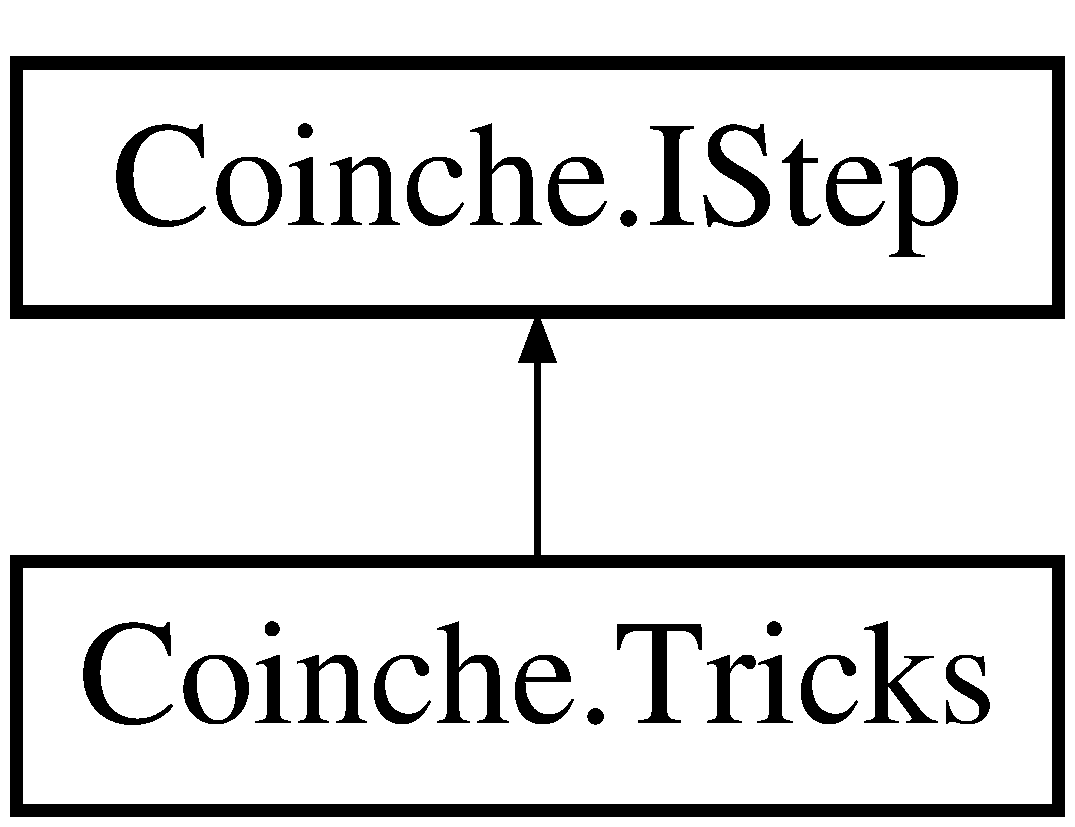
\includegraphics[height=2.000000cm]{class_coinche_1_1_tricks}
\end{center}
\end{figure}
\subsection*{Public Member Functions}
\begin{DoxyCompactItemize}
\item 
\hyperlink{class_coinche_1_1_tricks_afba8d7dcb751a3dde112f7f702399d00}{Tricks} ()
\begin{DoxyCompactList}\small\item\em simple constructor \end{DoxyCompactList}\end{DoxyCompactItemize}
\subsection*{Private Member Functions}
\begin{DoxyCompactItemize}
\item 
void I\+Step. \hyperlink{class_coinche_1_1_tricks_ade6668950abaf544373d90516821eab1}{Reset} ()
\begin{DoxyCompactList}\small\item\em reset the step \end{DoxyCompactList}\item 
\hyperlink{class_coinche_1_1_tools_1_1_game_info}{Game\+Info} I\+Step. \hyperlink{class_coinche_1_1_tricks_a7d2fedfa7e574f3570d1be83943fa953}{Prepare\+Step} (\hyperlink{class_coinche_1_1_player}{Player} player, int team\+Contract)
\begin{DoxyCompactList}\small\item\em prepare the players for the next step \end{DoxyCompactList}\item 
\hyperlink{class_coinche_1_1_tools_1_1_game_info}{Game\+Info} I\+Step. \hyperlink{class_coinche_1_1_tricks_ae9cd4602740f7612010fac07af2997a8}{Do\+Step} (\hyperlink{class_coinche_1_1_player}{Player} player, string msg, Boolean all\+Assets, Boolean none\+Assets, Card\+Color color\+Bet, int first\+Player)
\begin{DoxyCompactList}\small\item\em rules of the current step applied with the players messages \end{DoxyCompactList}\item 
\mbox{\Hypertarget{class_coinche_1_1_tricks_a55a862ddde306c1f698777f51bd482f8}\label{class_coinche_1_1_tricks_a55a862ddde306c1f698777f51bd482f8}} 
string {\bfseries Belotte\+Rebelotte} (\hyperlink{class_coinche_1_1_player}{Player} player, Boolean all\+Assets, Boolean none\+Assets, Card\+Color color\+Bet, \hyperlink{class_coinche_1_1_card}{Card} card\+Played)
\item 
\mbox{\Hypertarget{class_coinche_1_1_tricks_ac1bda0bbf8a4718f5d09b49de24a2996}\label{class_coinche_1_1_tricks_ac1bda0bbf8a4718f5d09b49de24a2996}} 
\hyperlink{class_coinche_1_1_tools_1_1_game_info}{Game\+Info} {\bfseries Collect\+Trick} (\hyperlink{class_coinche_1_1_tools_1_1_game_info}{Game\+Info} infos, int \hyperlink{class_coinche_1_1_tricks_a234997b0338ef3f6fe31159e789ff926}{Trick\+Index}, Boolean all\+Assets, Boolean none\+Assets, Card\+Color color\+Bet)
\item 
\mbox{\Hypertarget{class_coinche_1_1_tricks_abd2bd2645b75d22a8c0d96134916c576}\label{class_coinche_1_1_tricks_abd2bd2645b75d22a8c0d96134916c576}} 
int {\bfseries Count\+Round\+Points} (int num\+Round, Boolean all\+Assets, Boolean none\+Assets, Card\+Color color\+Bet)
\item 
\hyperlink{class_coinche_1_1_tools_1_1_game_info}{Game\+Info} I\+Step. \hyperlink{class_coinche_1_1_tricks_a298a3f9c18af5a9e2ab7da3c7509075a}{Invalid\+Turn} (\hyperlink{class_coinche_1_1_player}{Player} player)
\begin{DoxyCompactList}\small\item\em function called if it wasn\textquotesingle{}t the right turn to play \end{DoxyCompactList}\item 
string I\+Step. \hyperlink{class_coinche_1_1_tricks_afa44486bcd0e3ce034330d8c0f0d36eb}{Step\+Over} ()
\begin{DoxyCompactList}\small\item\em function called when the step is over \end{DoxyCompactList}\end{DoxyCompactItemize}
\subsection*{Private Attributes}
\begin{DoxyCompactItemize}
\item 
\hyperlink{class_coinche_1_1_board}{Board} \hyperlink{class_coinche_1_1_tricks_a98e0ea7da7ca1f0e85513c91bf311fc6}{Game\+Board}
\begin{DoxyCompactList}\small\item\em game board \end{DoxyCompactList}\item 
int \hyperlink{class_coinche_1_1_tricks_a234997b0338ef3f6fe31159e789ff926}{Trick\+Index}
\begin{DoxyCompactList}\small\item\em the number of the current trick \end{DoxyCompactList}\item 
int \hyperlink{class_coinche_1_1_tricks_a989d0fe41242144d3b51145cce83195f}{First}
\begin{DoxyCompactList}\small\item\em the index of the first player of the trick \end{DoxyCompactList}\item 
Boolean \hyperlink{class_coinche_1_1_tricks_a52b326e759bb3b8db0eb4aac4673c84e}{belotte}
\begin{DoxyCompactList}\small\item\em true if a player played a belotte \end{DoxyCompactList}\item 
int \hyperlink{class_coinche_1_1_tricks_ad6c681dc74c4d3e916803c90bb8cb446}{belotte\+\_\+player}
\begin{DoxyCompactList}\small\item\em index of the player who played the belotte \end{DoxyCompactList}\end{DoxyCompactItemize}


\subsection{Detailed Description}
class representing the tricks step 



\subsection{Constructor \& Destructor Documentation}
\mbox{\Hypertarget{class_coinche_1_1_tricks_afba8d7dcb751a3dde112f7f702399d00}\label{class_coinche_1_1_tricks_afba8d7dcb751a3dde112f7f702399d00}} 
\index{Coinche\+::\+Tricks@{Coinche\+::\+Tricks}!Tricks@{Tricks}}
\index{Tricks@{Tricks}!Coinche\+::\+Tricks@{Coinche\+::\+Tricks}}
\subsubsection{\texorpdfstring{Tricks()}{Tricks()}}
{\footnotesize\ttfamily Coinche.\+Tricks.\+Tricks (\begin{DoxyParamCaption}{ }\end{DoxyParamCaption})\hspace{0.3cm}{\ttfamily [inline]}}



simple constructor 



\subsection{Member Function Documentation}
\mbox{\Hypertarget{class_coinche_1_1_tricks_ae9cd4602740f7612010fac07af2997a8}\label{class_coinche_1_1_tricks_ae9cd4602740f7612010fac07af2997a8}} 
\index{Coinche\+::\+Tricks@{Coinche\+::\+Tricks}!Do\+Step@{Do\+Step}}
\index{Do\+Step@{Do\+Step}!Coinche\+::\+Tricks@{Coinche\+::\+Tricks}}
\subsubsection{\texorpdfstring{Do\+Step()}{DoStep()}}
{\footnotesize\ttfamily \hyperlink{class_coinche_1_1_tools_1_1_game_info}{Game\+Info} I\+Step. Coinche.\+Tricks.\+Do\+Step (\begin{DoxyParamCaption}\item[{\hyperlink{class_coinche_1_1_player}{Player}}]{player,  }\item[{string}]{msg,  }\item[{Boolean}]{all\+Assets,  }\item[{Boolean}]{none\+Assets,  }\item[{Card\+Color}]{color\+Bet,  }\item[{int}]{first\+Player }\end{DoxyParamCaption})\hspace{0.3cm}{\ttfamily [inline]}, {\ttfamily [private]}}



rules of the current step applied with the players messages 


\begin{DoxyParams}{Parameters}
{\em player} & \\
\hline
{\em msg} & \\
\hline
{\em all\+Assets} & \\
\hline
{\em none\+Assets} & \\
\hline
{\em color\+Bet} & \\
\hline
{\em first\+Player} & \\
\hline
\end{DoxyParams}
\begin{DoxyReturn}{Returns}
a Game\+Info instance to tell players what happened
\end{DoxyReturn}


Implements \hyperlink{interface_coinche_1_1_i_step_a1b410159a7988ae4e75154539715e7ba}{Coinche.\+I\+Step}.

\mbox{\Hypertarget{class_coinche_1_1_tricks_a298a3f9c18af5a9e2ab7da3c7509075a}\label{class_coinche_1_1_tricks_a298a3f9c18af5a9e2ab7da3c7509075a}} 
\index{Coinche\+::\+Tricks@{Coinche\+::\+Tricks}!Invalid\+Turn@{Invalid\+Turn}}
\index{Invalid\+Turn@{Invalid\+Turn}!Coinche\+::\+Tricks@{Coinche\+::\+Tricks}}
\subsubsection{\texorpdfstring{Invalid\+Turn()}{InvalidTurn()}}
{\footnotesize\ttfamily \hyperlink{class_coinche_1_1_tools_1_1_game_info}{Game\+Info} I\+Step. Coinche.\+Tricks.\+Invalid\+Turn (\begin{DoxyParamCaption}\item[{\hyperlink{class_coinche_1_1_player}{Player}}]{player }\end{DoxyParamCaption})\hspace{0.3cm}{\ttfamily [inline]}, {\ttfamily [private]}}



function called if it wasn\textquotesingle{}t the right turn to play 


\begin{DoxyParams}{Parameters}
{\em player} & \\
\hline
\end{DoxyParams}
\begin{DoxyReturn}{Returns}
a Game\+Info instance to inform the player it wasn\textquotesingle{}t his turn to play
\end{DoxyReturn}


Implements \hyperlink{interface_coinche_1_1_i_step_afc64813670860f5ee0829264751abc0a}{Coinche.\+I\+Step}.

\mbox{\Hypertarget{class_coinche_1_1_tricks_a7d2fedfa7e574f3570d1be83943fa953}\label{class_coinche_1_1_tricks_a7d2fedfa7e574f3570d1be83943fa953}} 
\index{Coinche\+::\+Tricks@{Coinche\+::\+Tricks}!Prepare\+Step@{Prepare\+Step}}
\index{Prepare\+Step@{Prepare\+Step}!Coinche\+::\+Tricks@{Coinche\+::\+Tricks}}
\subsubsection{\texorpdfstring{Prepare\+Step()}{PrepareStep()}}
{\footnotesize\ttfamily \hyperlink{class_coinche_1_1_tools_1_1_game_info}{Game\+Info} I\+Step. Coinche.\+Tricks.\+Prepare\+Step (\begin{DoxyParamCaption}\item[{\hyperlink{class_coinche_1_1_player}{Player}}]{player,  }\item[{int}]{team\+Contract }\end{DoxyParamCaption})\hspace{0.3cm}{\ttfamily [inline]}, {\ttfamily [private]}}



prepare the players for the next step 


\begin{DoxyParams}{Parameters}
{\em player} & \\
\hline
{\em team\+Contract} & \\
\hline
\end{DoxyParams}
\begin{DoxyReturn}{Returns}
infos to tell them what to do
\end{DoxyReturn}


Implements \hyperlink{interface_coinche_1_1_i_step_ada17a0e471c5afbc7e4f4acc434cdd76}{Coinche.\+I\+Step}.

\mbox{\Hypertarget{class_coinche_1_1_tricks_ade6668950abaf544373d90516821eab1}\label{class_coinche_1_1_tricks_ade6668950abaf544373d90516821eab1}} 
\index{Coinche\+::\+Tricks@{Coinche\+::\+Tricks}!Reset@{Reset}}
\index{Reset@{Reset}!Coinche\+::\+Tricks@{Coinche\+::\+Tricks}}
\subsubsection{\texorpdfstring{Reset()}{Reset()}}
{\footnotesize\ttfamily void I\+Step. Coinche.\+Tricks.\+Reset (\begin{DoxyParamCaption}{ }\end{DoxyParamCaption})\hspace{0.3cm}{\ttfamily [inline]}, {\ttfamily [private]}}



reset the step 



Implements \hyperlink{interface_coinche_1_1_i_step_a764f20494a35e9b006c6495a38717e9a}{Coinche.\+I\+Step}.

\mbox{\Hypertarget{class_coinche_1_1_tricks_afa44486bcd0e3ce034330d8c0f0d36eb}\label{class_coinche_1_1_tricks_afa44486bcd0e3ce034330d8c0f0d36eb}} 
\index{Coinche\+::\+Tricks@{Coinche\+::\+Tricks}!Step\+Over@{Step\+Over}}
\index{Step\+Over@{Step\+Over}!Coinche\+::\+Tricks@{Coinche\+::\+Tricks}}
\subsubsection{\texorpdfstring{Step\+Over()}{StepOver()}}
{\footnotesize\ttfamily string I\+Step. Coinche.\+Tricks.\+Step\+Over (\begin{DoxyParamCaption}{ }\end{DoxyParamCaption})\hspace{0.3cm}{\ttfamily [inline]}, {\ttfamily [private]}}



function called when the step is over 

\begin{DoxyReturn}{Returns}
a string to tell players the step is over
\end{DoxyReturn}


Implements \hyperlink{interface_coinche_1_1_i_step_a86ef55b4c36ffa27f5fa18a10e9a61a0}{Coinche.\+I\+Step}.



\subsection{Member Data Documentation}
\mbox{\Hypertarget{class_coinche_1_1_tricks_a52b326e759bb3b8db0eb4aac4673c84e}\label{class_coinche_1_1_tricks_a52b326e759bb3b8db0eb4aac4673c84e}} 
\index{Coinche\+::\+Tricks@{Coinche\+::\+Tricks}!belotte@{belotte}}
\index{belotte@{belotte}!Coinche\+::\+Tricks@{Coinche\+::\+Tricks}}
\subsubsection{\texorpdfstring{belotte}{belotte}}
{\footnotesize\ttfamily Boolean Coinche.\+Tricks.\+belotte\hspace{0.3cm}{\ttfamily [private]}}



true if a player played a belotte 

\mbox{\Hypertarget{class_coinche_1_1_tricks_ad6c681dc74c4d3e916803c90bb8cb446}\label{class_coinche_1_1_tricks_ad6c681dc74c4d3e916803c90bb8cb446}} 
\index{Coinche\+::\+Tricks@{Coinche\+::\+Tricks}!belotte\+\_\+player@{belotte\+\_\+player}}
\index{belotte\+\_\+player@{belotte\+\_\+player}!Coinche\+::\+Tricks@{Coinche\+::\+Tricks}}
\subsubsection{\texorpdfstring{belotte\+\_\+player}{belotte\_player}}
{\footnotesize\ttfamily int Coinche.\+Tricks.\+belotte\+\_\+player\hspace{0.3cm}{\ttfamily [private]}}



index of the player who played the belotte 

\mbox{\Hypertarget{class_coinche_1_1_tricks_a989d0fe41242144d3b51145cce83195f}\label{class_coinche_1_1_tricks_a989d0fe41242144d3b51145cce83195f}} 
\index{Coinche\+::\+Tricks@{Coinche\+::\+Tricks}!First@{First}}
\index{First@{First}!Coinche\+::\+Tricks@{Coinche\+::\+Tricks}}
\subsubsection{\texorpdfstring{First}{First}}
{\footnotesize\ttfamily int Coinche.\+Tricks.\+First\hspace{0.3cm}{\ttfamily [private]}}



the index of the first player of the trick 

\mbox{\Hypertarget{class_coinche_1_1_tricks_a98e0ea7da7ca1f0e85513c91bf311fc6}\label{class_coinche_1_1_tricks_a98e0ea7da7ca1f0e85513c91bf311fc6}} 
\index{Coinche\+::\+Tricks@{Coinche\+::\+Tricks}!Game\+Board@{Game\+Board}}
\index{Game\+Board@{Game\+Board}!Coinche\+::\+Tricks@{Coinche\+::\+Tricks}}
\subsubsection{\texorpdfstring{Game\+Board}{GameBoard}}
{\footnotesize\ttfamily \hyperlink{class_coinche_1_1_board}{Board} Coinche.\+Tricks.\+Game\+Board\hspace{0.3cm}{\ttfamily [private]}}



game board 

\mbox{\Hypertarget{class_coinche_1_1_tricks_a234997b0338ef3f6fe31159e789ff926}\label{class_coinche_1_1_tricks_a234997b0338ef3f6fe31159e789ff926}} 
\index{Coinche\+::\+Tricks@{Coinche\+::\+Tricks}!Trick\+Index@{Trick\+Index}}
\index{Trick\+Index@{Trick\+Index}!Coinche\+::\+Tricks@{Coinche\+::\+Tricks}}
\subsubsection{\texorpdfstring{Trick\+Index}{TrickIndex}}
{\footnotesize\ttfamily int Coinche.\+Tricks.\+Trick\+Index\hspace{0.3cm}{\ttfamily [private]}}



the number of the current trick 



The documentation for this class was generated from the following file\+:\begin{DoxyCompactItemize}
\item 
Server/\+Game\+Rules/\+Steps/\+Tricks/Tricks.\+cs\end{DoxyCompactItemize}

%--- End generated contents ---

% Index
\backmatter
\newpage
\phantomsection
\clearemptydoublepage
\addcontentsline{toc}{chapter}{Index}
\printindex

\end{document}
